\documentclass[UTF8]{ctexart}
% \documentclass[12pt]{report}
\usepackage{ctex}
\usepackage{setspace}
\usepackage{graphicx}
\usepackage{float}
\usepackage{subfigure}
\usepackage{geometry}
\usepackage{makecell}
\usepackage[table,xcdraw]{xcolor}
\usepackage{listings}
\geometry{a4paper,scale=0.8}
\setCJKmainfont{SimSun}
\renewcommand{\normalsize}{\fontsize{12pt}{15pt}\selectfont}
\setstretch{1.0}

\begin{document}


\title{智能计算芯片导论期末课程设计报告 \\——基于RISCV向量扩展指令集的VPU设计}
\maketitle
\begin{center}
	22307130445 贾梓越
\end{center}

\section{设计目标}
使用Verilog搭建一个基于RISCV向量扩展指令集的VPU。使用汇编语言实现8*8的矩阵乘加运算,使用Vivado进行仿真验证,
并进行性能分析,测试延迟,仿真功耗以及LUT/DSP/BRAM的占用率。最后尝试对架构和软件进行优化,并分析优化的效果。
\section{设计架构}
\subsection{整体架构}
整体架构如图1所示,VPU一共分为四级流水线,每个指令的执行需要经过四个周期:取指,译码并取数,执行或访存,最后写回。

指令缓存用于存储需要执行的指令,由一个指令计数器PC作为读取地址逐个读取,每个指令的位宽为32位,与RISCV的指令集兼容。

指令读出后经过译码器,将指令根据指令类型拆分出为立即数、标量和矢量的源寄存器地址和目标寄存器地址,送往立即数生成模块、标量寄存器和矢量寄存器。
标量寄存器和矢量寄存器用于存储指令执行过程中的中间结果。
设计的数据位宽为32,向量寄存器的向量长度为8,因此每个单元位宽为32*8=256位。
向量寄存器和标量寄存器各32个,对应5位寄存器地址,这也与RISCV指令集的寄存器地址位宽相同。
由于立即数需要与标量寄存器的读取结果相加,或者直接写入标量寄存器中,因此在译码时将立即数的位宽拓展为32位,便于和一般数据相加。

标量寄存器读取的数据有三种通路:(1)和立即数产生单元的输出数据相加后作为访存的地址访问标量缓存或者矢量缓存;(2)直接输入乘加运算单元进行计算;(3)写入标量缓存

矢量寄存器读取的数据则有两种通路:(1)直接输入乘加运算单元进行计算;(2)写入矢量缓存。

对于乘加单元,考虑到只有一级流水,需要在一个周期内完成乘加运算,本次设计只进行整型数据,即32位有符号整数的乘加运算,也可以拓展到定点数的运算。
但是如果需要进行浮点数的运算,就需要多个周期完成,控制逻辑的时序就需要修改,较为复杂,本次设计不进行浮点数运算。

除了基本的存储和计算单元,还需要一个整体的控制单元负责控制各个存储器的读写使能信号和寄存器的写使能信号,以及一些数据选择器的选择信号。

\begin{figure}[htbp]
    \centering
    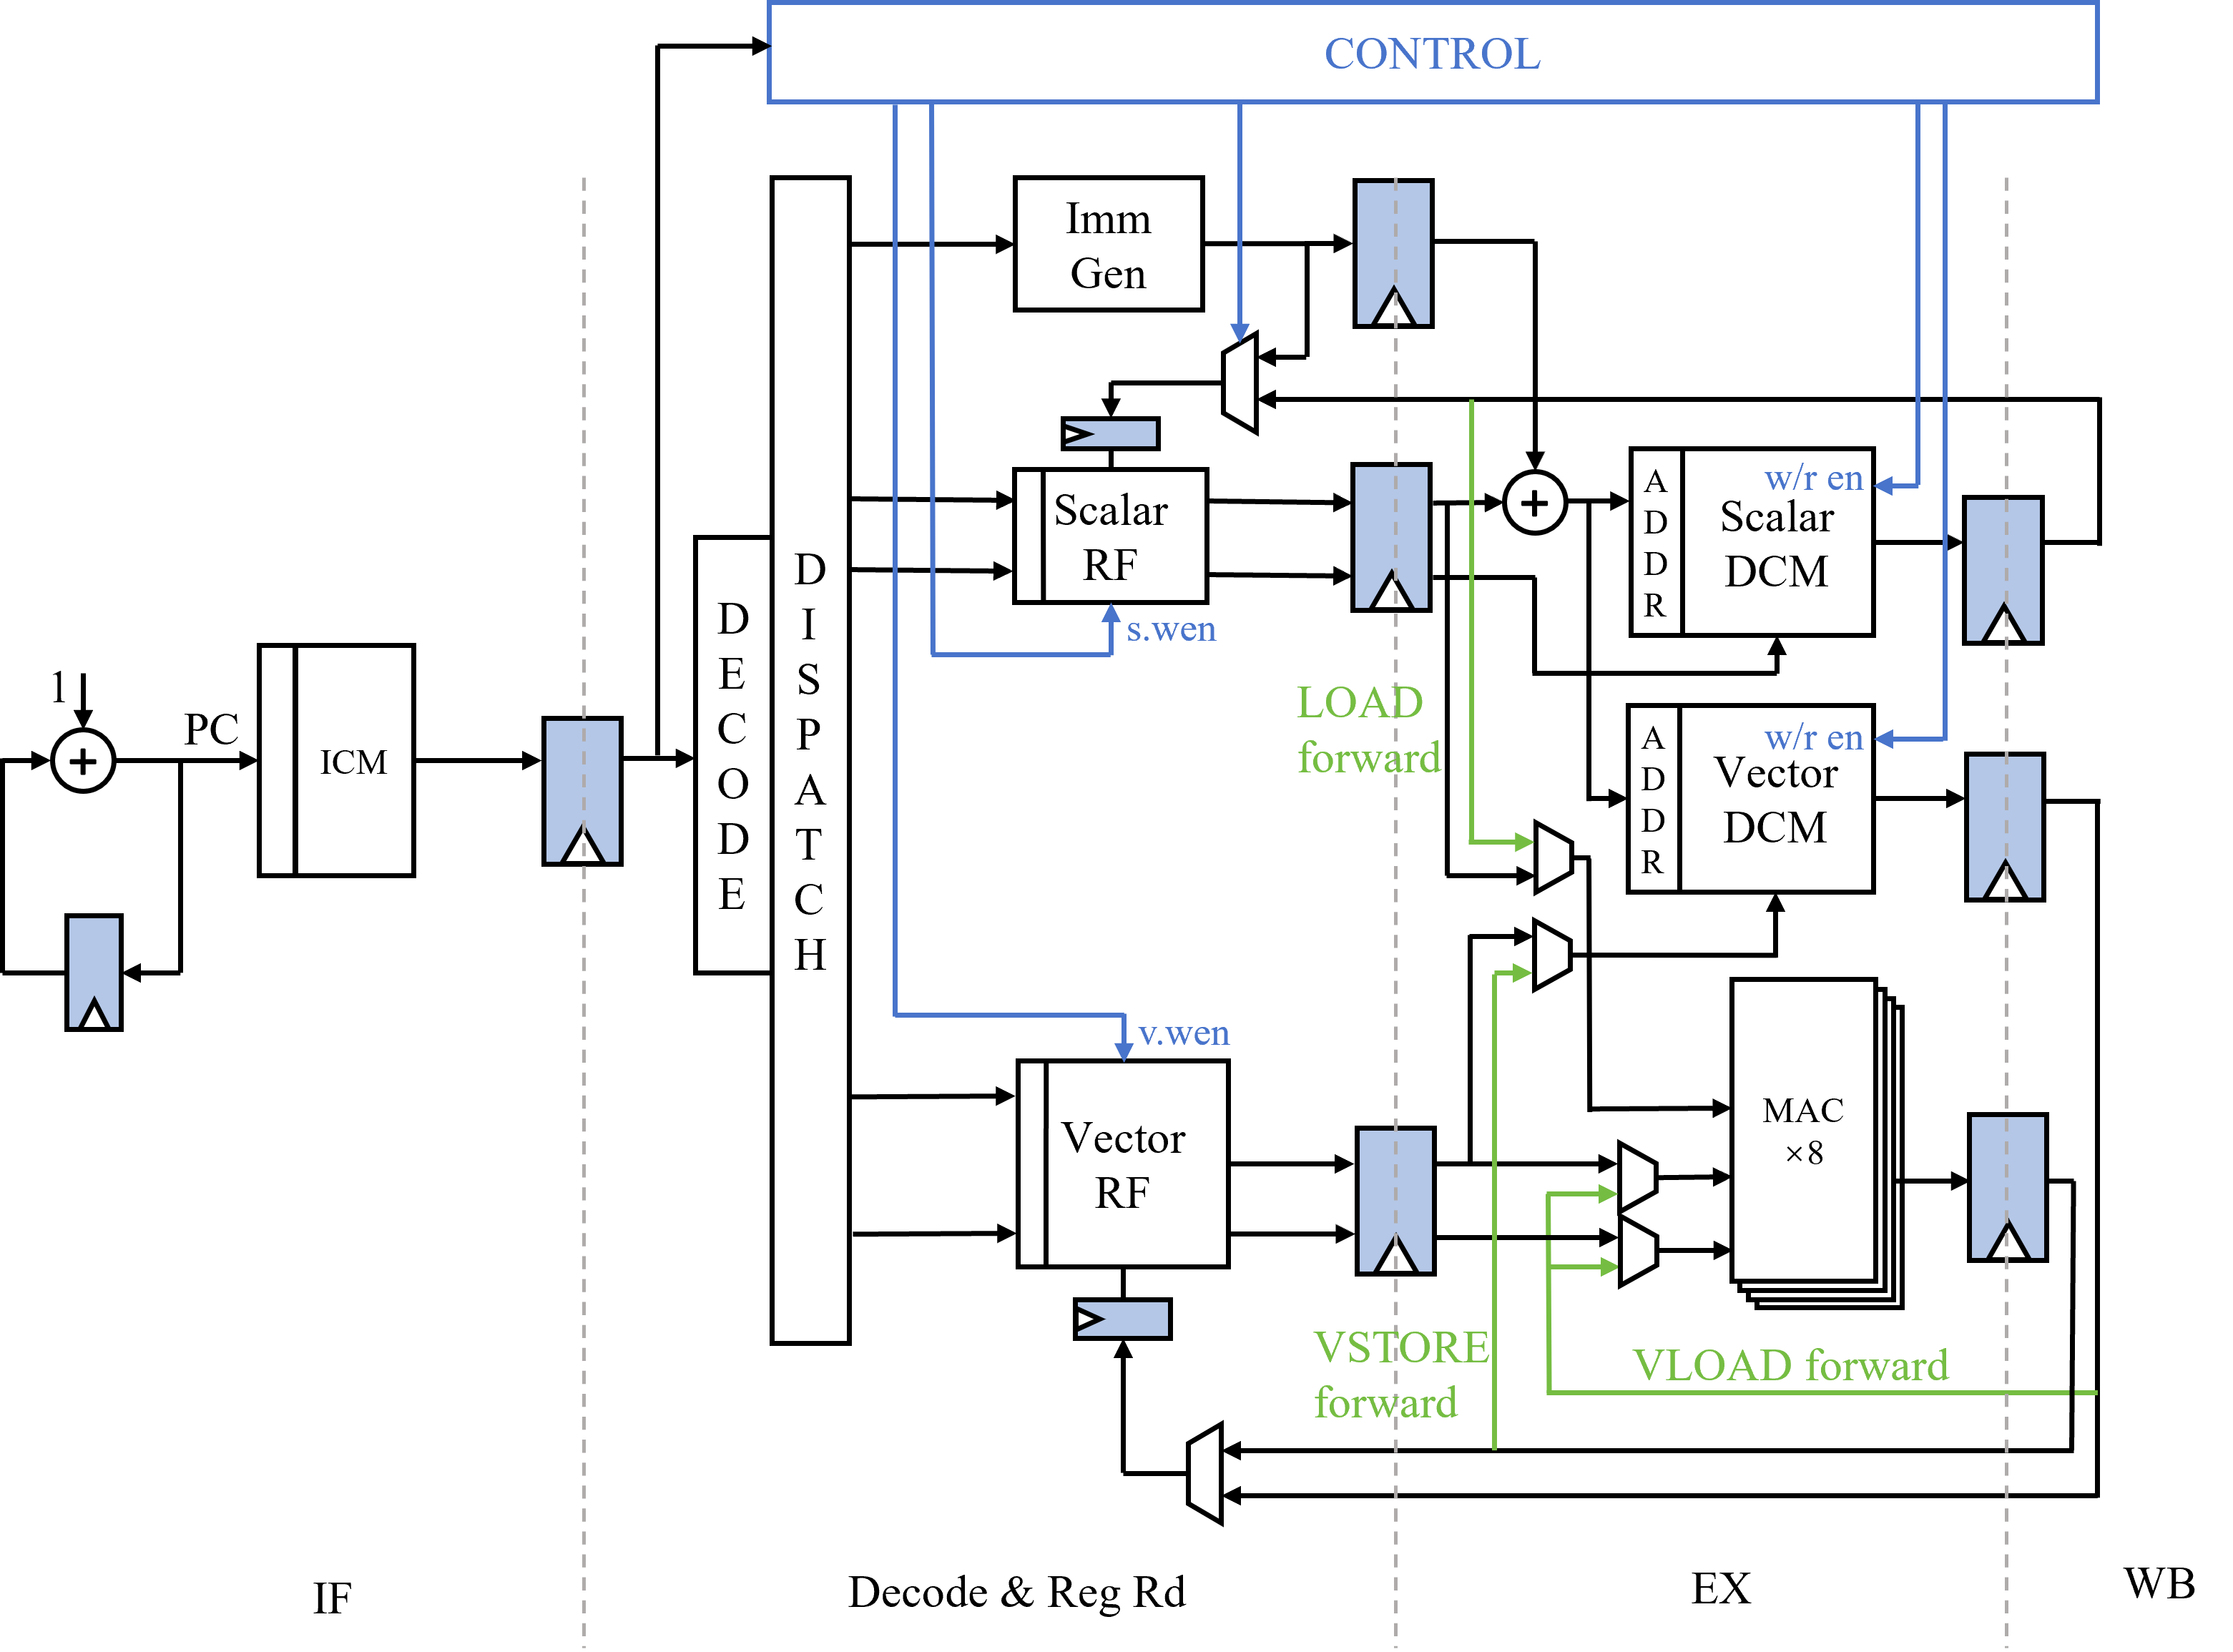
\includegraphics[width=16cm]{pic/Structure.png}
    \caption{架构图}
\end{figure}

\subsection{指令集设计}
矢量处理器可以进行矢量和标量的运算,支持RISCV矢量扩展的SIMD指令。使用的指令集包括MOV,LOAD,VLOAD,MAC,STORE,VSTORE。格式如图2所示。
\begin{figure}[htbp]
    \centering
    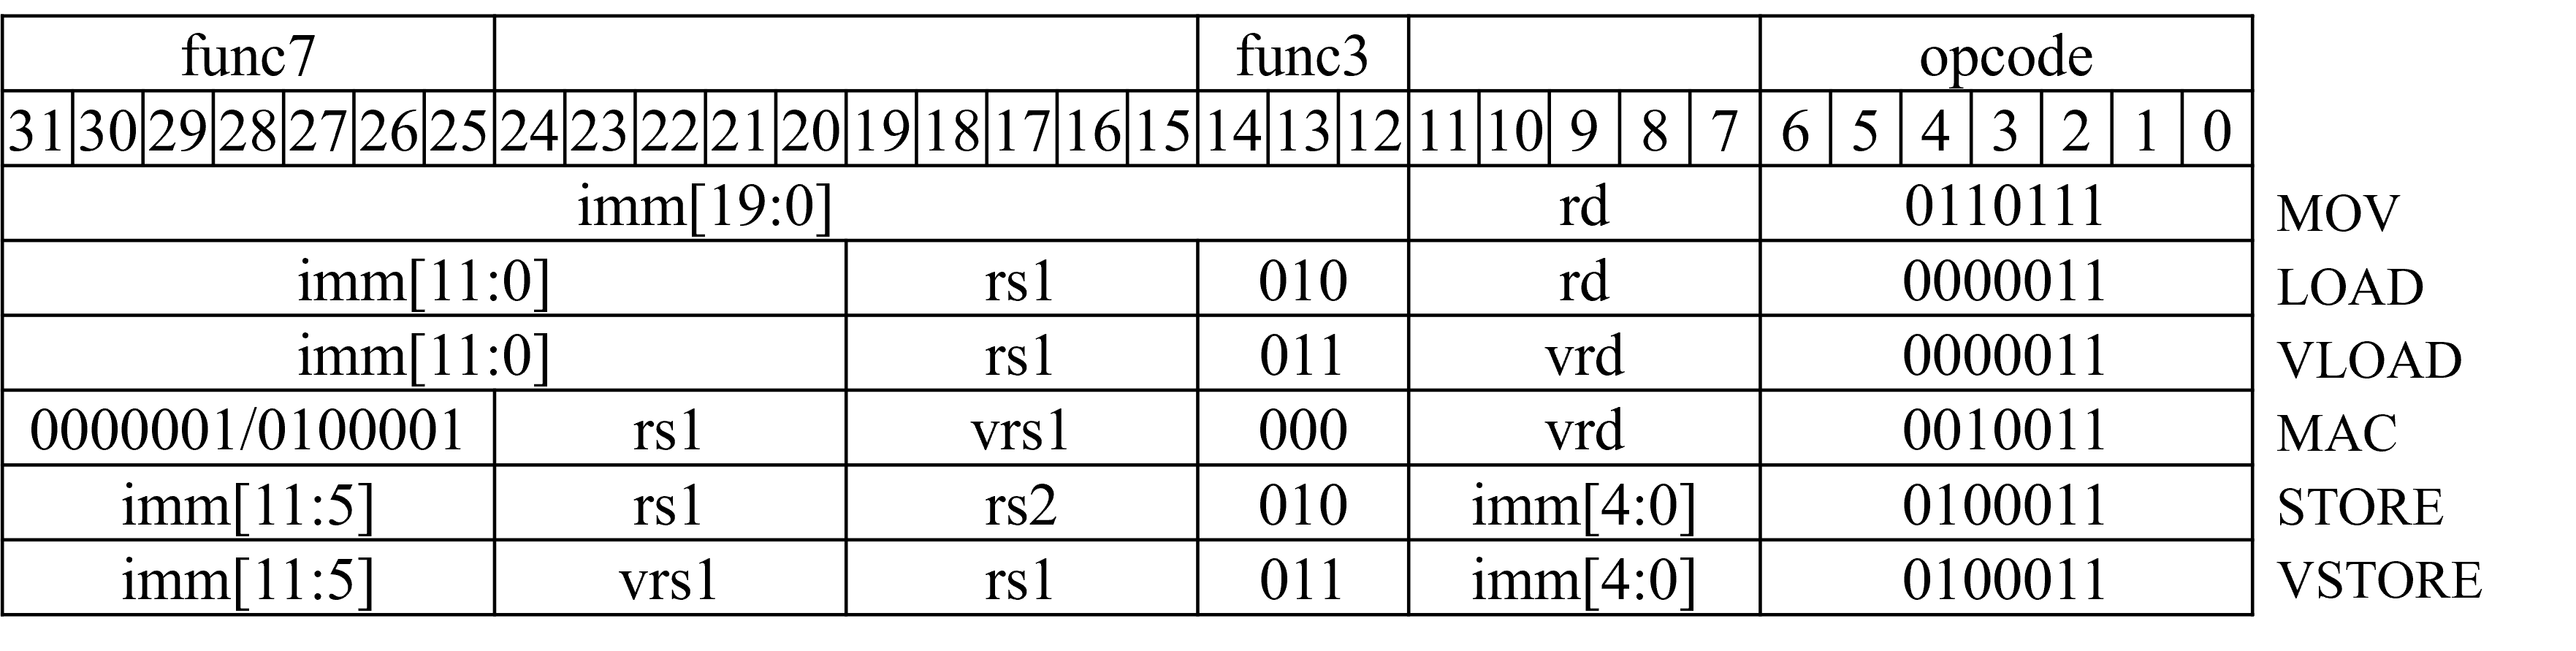
\includegraphics[width=18cm]{pic/instr_set.png}
    \caption{指令集格式设计}
\end{figure}

MOV指令使用的操作码对应RISCV指令集中的AUIPC,将立即数直接加载到标量寄存器中,可以表示为
\begin{lstlisting}
    imm -> ScalarRF[rd]
\end{lstlisting}

LOAD和VLOAD指令的操作码都对应RISCV指令集中的LOAD,用func3码段进行区分,将源寄存器中的数加上立即数偏移量作为访存的地址,将存储器的读取结果写入寄存器堆中,
可以表示为
\begin{lstlisting}
    ScalarDCM[ScalarRF[rs1] + imm] -> ScalarRF[rd]
\end{lstlisting}
或者
\begin{lstlisting}
    VectorDCM[ScalarRF[rs1] + imm] -> VectorRF[vrd]
\end{lstlisting}

MAC指令的操作码对应RISCV指令集中的计算类指令,为了和其他指令冲突,将func7的最低为设为1,同时func7的第6位作为配置位,如果是1则是reset模式,是0则是计算模式。
计算时先将目标矢量寄存器的数据和另一个矢量寄存器的数据读出,即使用vrd和vrs1作为矢量寄存器的地址读数,进行乘累加运算后再写回到目标矢量寄存器中。
此时矢量寄存器需要一次读出两个数据,因此需要两个端口。
可以表示为
\begin{lstlisting}
    Scalar[rs1] * VectorRF[vrs1] + VectorRF[vrd(vrs2)] -> VectorRF[vrd]
\end{lstlisting} 
或者
\begin{lstlisting}
    VectorRF[vrs1] -> VectorRF[vrd]
\end{lstlisting}

STORE和VSTORE的操作码对应RISCV指令集中的存储类指令,两种指令用func3码段进行区分,将源寄存器读出的数据加上立即数偏移量作为访存的地址,
将寄存器堆中的数据写入存储器中。STORE指令用来存储标量,此时标量寄存器需要同时读出访存地址和存储的数据,因此需要两个端口。指令功能可以表示为
\begin{lstlisting}
    ScalarRF[rs2]  -> ScalarDCM[ScalarRF[rs1] + imm]
\end{lstlisting} 
或者
\begin{lstlisting}
    VectorRF[vrs1] -> VectorDCM[ScalarRF[rs1] + imm]
\end{lstlisting} 

\subsection{指令执行过程}
控制模块的功能比较复杂,使能和选择信号的产生需要结合指令内容和不同流水级,按照正确的时序给出,这与每个指令的执行顺序有关。
下面将结合每个指令的执行过程具体说明控制信号的产生逻辑。
\subsubsection{MOV指令}
译码器接收到指令的同时,经过一个组合电路产生立即数,同时标量寄存器的写地址(rd)也生成完毕,下一个周期写入标量寄存器。
因此,控制单元需要在接收到指令的同时产生标量寄存器的写使能信号(ScalarRegWriteEn),才能在下一个周期写入数据,同时标量寄存器输入数据的选择器(ScalarRegRdSel)也要切换到立即数的通路。

因此,对于MOV指令,rd,ScalarRegWriteEn和ScalarRegRdSel都是组合逻辑直接产生的,与译码在同一周期完成。

MOV指令是比较特殊的一条指令,在编写汇编程序时,首先要使用MOV对寄存器进行初始化,将希望访问的存储器地址通过立即数的形式直接写入寄存器,才能开始读取存储器的数据。否则就无法读取数据,也就无法开始计算。

\subsubsection{LOAD指令}
译码器收到指令,下一个周期从标量寄存器中读出数据并和立即数相加,此时需要存储器的读使能信号(ScalarMemRead)有效,下一个周期从存储器中读出数据,再下一个周期写回寄存器。

写回地址(rd)和写使能(ScalarRegWriteEn)需要在收到指令两个周期后输入到标量寄存器。
实际上寄存器输入的选择信号也需要在两个周期后产生,但是因为没有其他情况需要用立即数直接写入寄存器,所以只要保持选择存储器的数据通路即可。

因此,对于LOAD指令,ScalarMemRead在收到指令的下一个周期有效,rd和ScalarRegWriteEn需要经过两个周期的延时后才能更新。

\subsubsection{VLOAD指令}
VLOAD和LOAD的执行过程类似,接收到指令的下一个周期读出寄存器的数据并与偏移量相加产生地址,此时需要存储器的读使能信号(VectorMemRead)有效,下一个周期访问矢量存储器得到数据,
再下一个周期写回矢量寄存器,此时需要写回的数据选择器(VectorRegRdSel)选择矢量存储器的数据通路。

因此,和LOAD指令同理,VectorMemRead在收到指令的下一个周期有效,vrd,VectorRegWriteEn和VectorRegRdSel需要经过两个周期的延时后才能更新。

\subsubsection{MAC指令}
译码器接收到指令的下一个周期从矢量寄存器中读出两个矢量数据,从标量寄存器中读出一个标量数据,下一个周期进行乘累加运算,再下一个周期写回到矢量寄存器,此时需要写回的数据选择器(VectorRegRdSel)选择MAC的数据通路。

因此,对于MAC指令,vrd,VectorRegWriteEn和VectorRegRdSel需要经过两个周期的延时后才能更新。

\subsubsection{STORE指令}
接收到指令后,下一个周期从标量寄存器读出需要存储的数据和存储地址,此时存储器的写使能信号(ScalarMemWrite)有效,下一个周期写入标量存储器。

因此,对于STORE指令,ScalarMemWrite在收到指令的下一个周期更新。

\subsubsection{VSTORE指令}
VSTORE和STORE执行过程相似,只是写入的存储器变为矢量存储器。需要写使能信号(VectorMemWrite)在收到指令的下一个周期更新。

\subsection{前馈设计}
当出现写后读(RAW)时,可能导致数据冒险,在前一条指令未写回时就读出目标寄存器的数据,造成错误的结果。分析指令间的依赖关系,主要的RAW数据冒险分为两类:

\subsubsection{MAC指令造成的RAW}
执行MAC指令时操作数还没有加载到寄存器中,就被读出作为乘加运算的输入。

通过分析时序关系,第一个周期译码器接受到加载指令,第二个周期存储器地址生成,第三个周期数据读出,第四个周期数据写回,
而译码器接收到MAC指令的同时就需要读取寄存器的数。因此,从加载指令发出开始计算,需要经过三个周期再发出MAC指令才能避免RAW,如图3(a)所示。

具体而言,有分为两种情况,分别如图3(b)和(c)所示,情况1的加载指令在MAC指令前两个周期发出,当MAC需要读取操作数时,加载的数据正要写回,无法赶上,需要从访存的结果经过一个周期前馈到MAC模块。
情况2的加载指令在MAC指令前一个周期发出,当MAC需要读取操作数时,加载的数据刚刚从存储器输出,需要直接前馈到MAC模块。

需要实现这个前馈的控制,需要由控制器比对当前指令和之前一条指令,以及再之前一条指令的目标寄存器地址,来判断是否需要前馈,并选择正确的前馈通路。

\begin{figure}[htbp]
    \centering
    \subfigure[无RAW]{
        \label{Fig.sub.1}
        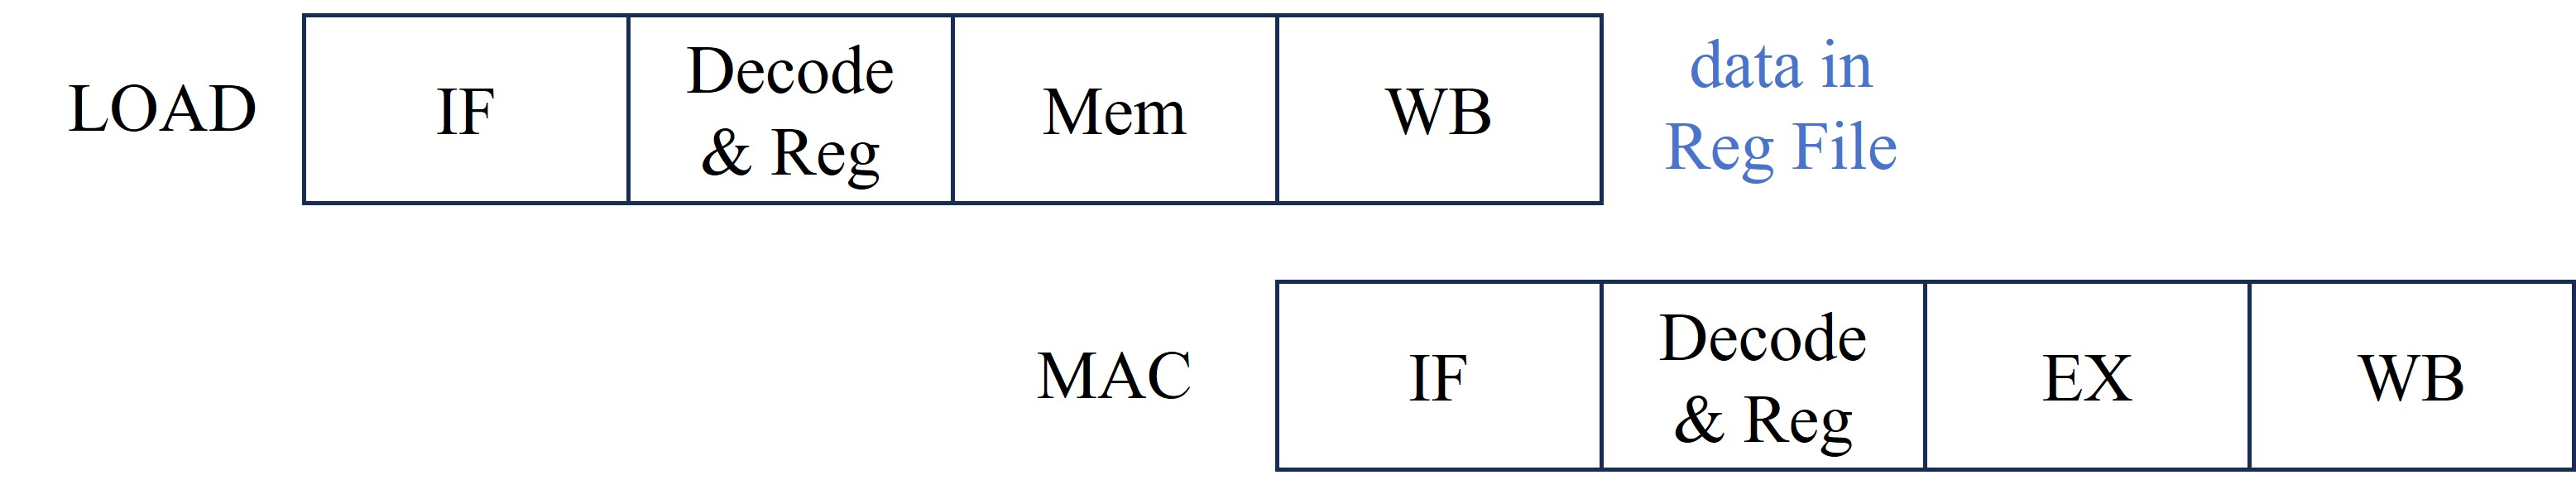
\includegraphics[width=14cm]{pic/MAC_RAW1.jpg}}
    \subfigure[RAW情况1]{
        \label{Fig.sub.2}
        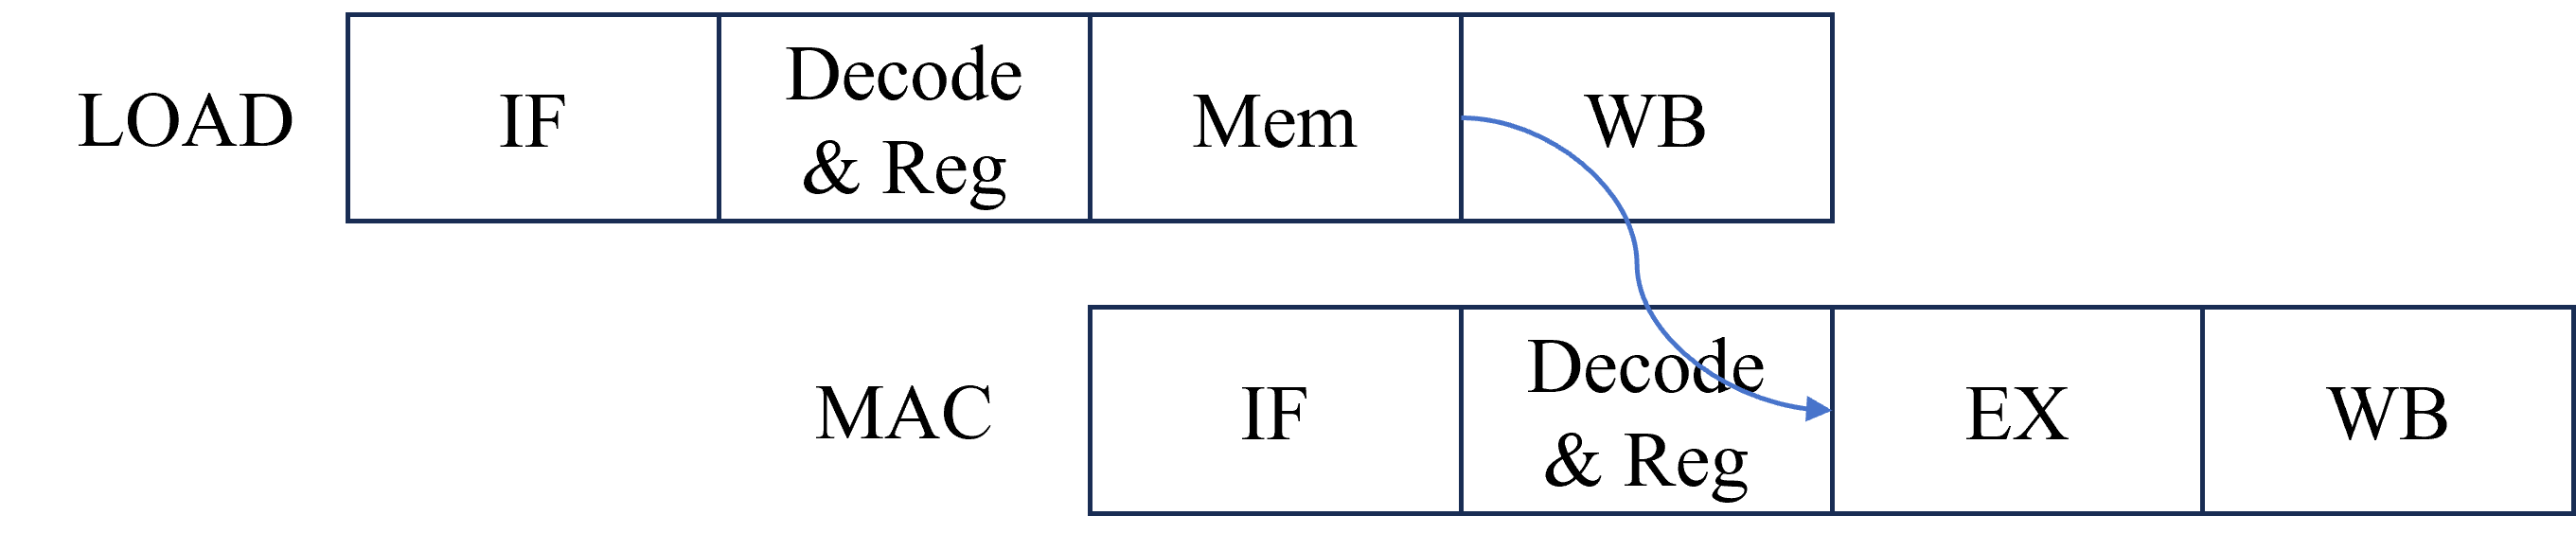
\includegraphics[width=12.7cm]{pic/MAC_RAW2.png}}
    \subfigure[RAW情况2]{
        \label{Fig.sub.3}
        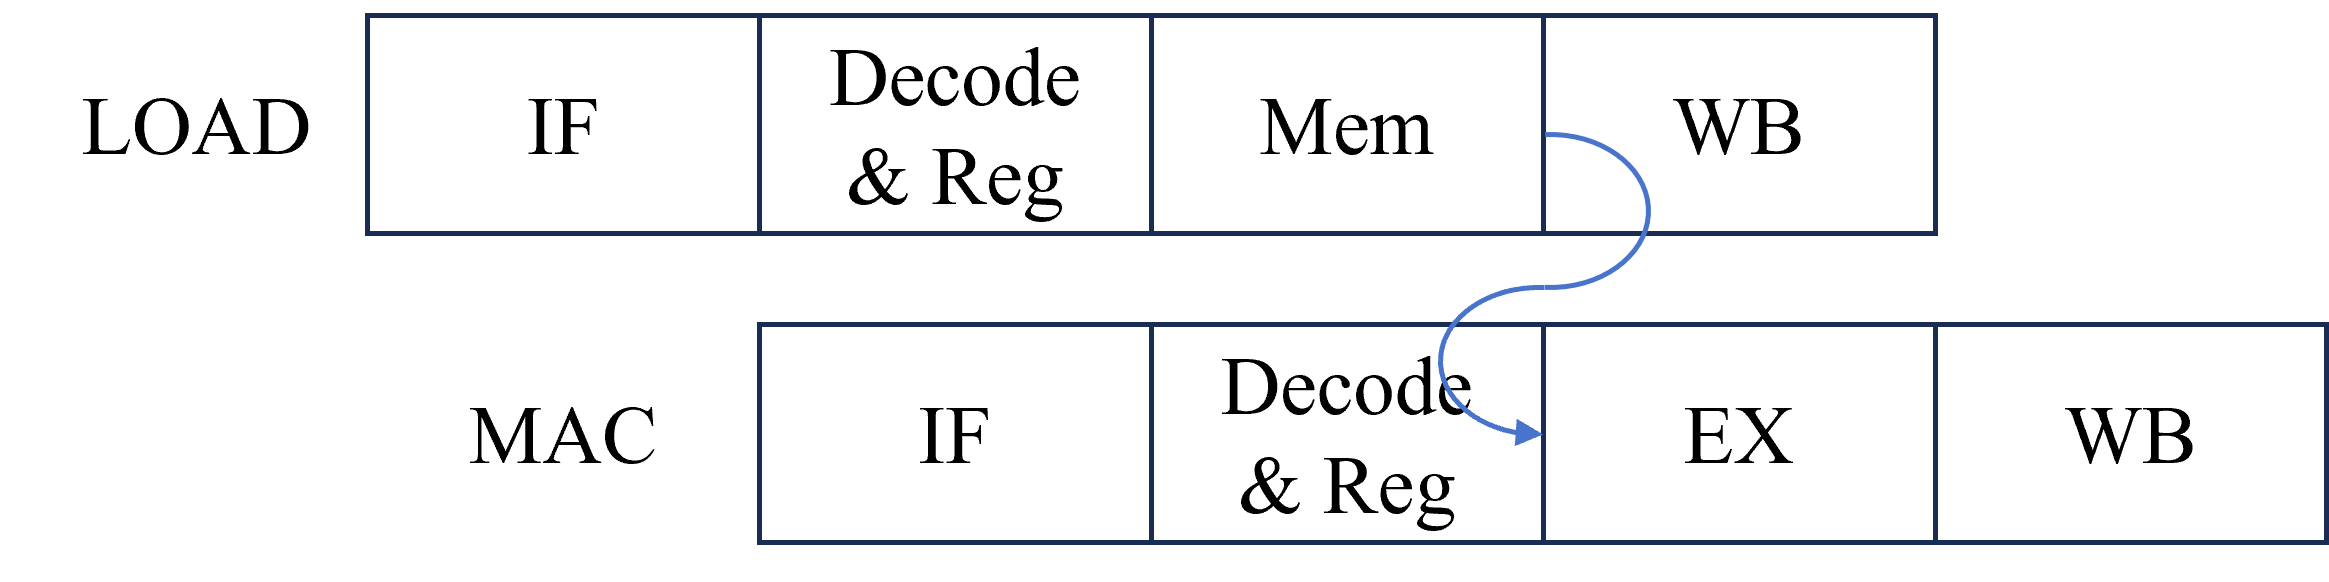
\includegraphics[width=11.1cm]{pic/MAC_RAW3.png}}
    \caption{MAC指令造成的RAW数据冒险情况}
    \label{Fig.main}
\end{figure}

\subsubsection{VSTORE造成的RAW}
执行VSTORE指令时,由于之前的运算操作还未写回,导致矢量寄存器还没有加载到数据,就被读出作为存储的地址。

一般而言,不会出现加载数据后立刻存储相同数据的情况,更常见的情况是计算完成后将结果存到存储器。在这个架构中,不支持标量的计算,因此不考虑标量的存储导致的RAW。

和前一种RAW类似,MAC指令在发出后需要经过三个周期才能发出VSTORE指令,如图4(a)所示。
具体的RAW有两种情况,如图4(a)和(b)所示,情况1中,需要将MAC的计算结果延时一个周期后前馈到矢量存储器。尽管看似仍有一个周期的延时,但是如果不使用前馈,而是写回寄存器,就会消耗两个周期,
因此前馈仍然是必要的。情况2中,对于VSTORE指令而言,MAC的结果出现的更晚,需要直接前馈到矢量存储器的输入端。

\begin{figure}[htbp]
    \centering
    \subfigure[无RAW]{
        \label{Fig.sub.1}
        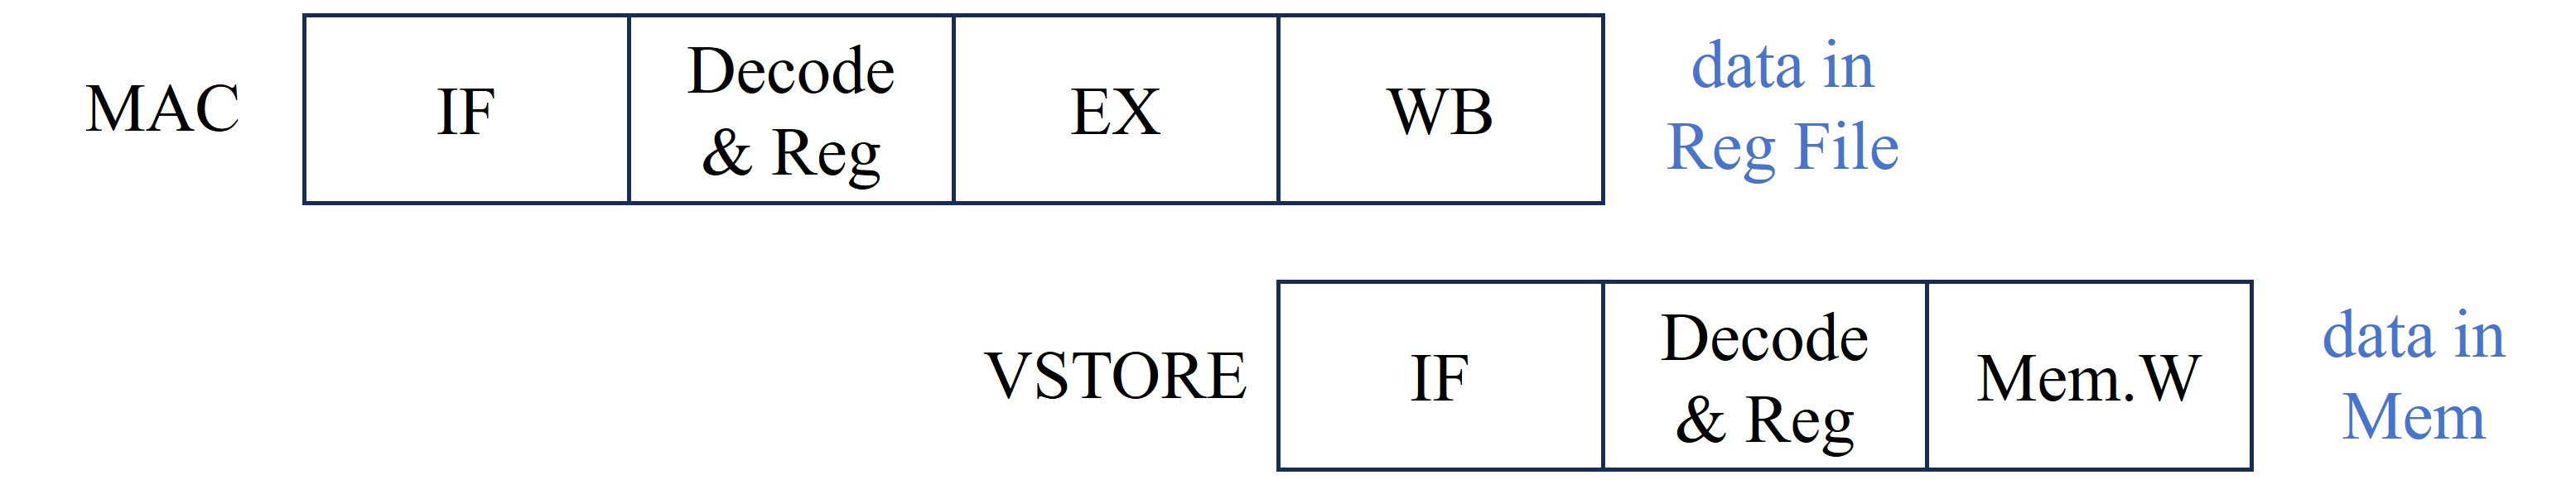
\includegraphics[width=14cm]{pic/STORE_RAW1.jpg}}
    \subfigure[RAW情况1]{
        \label{Fig.sub.2}
        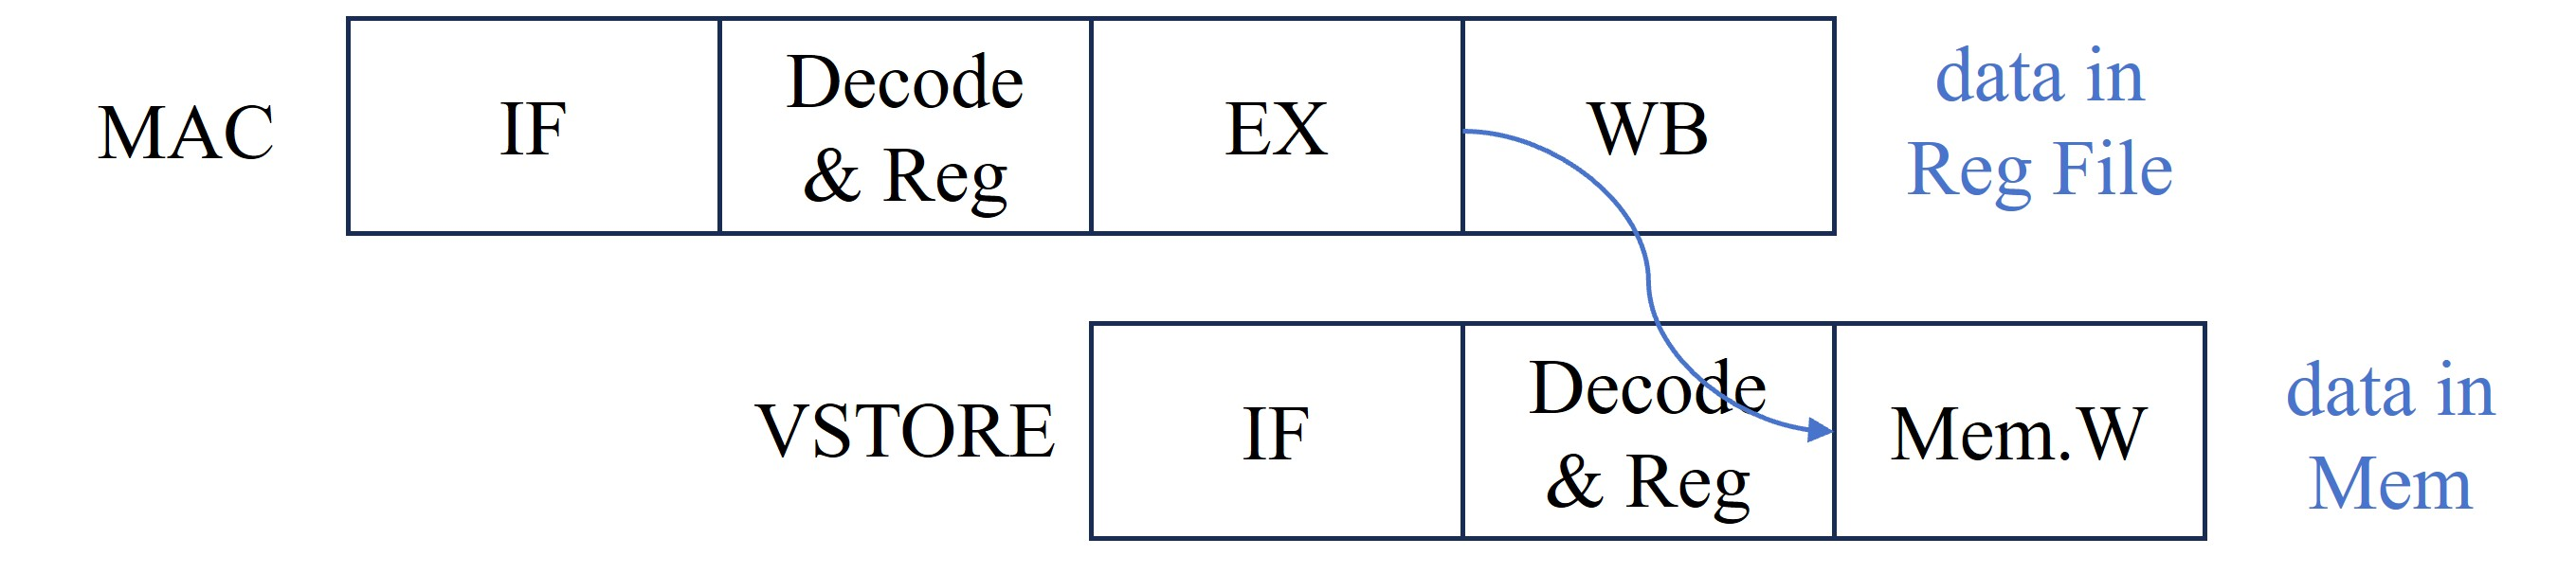
\includegraphics[width=12.7cm]{pic/STORE_RAW2.jpg}}
    \subfigure[RAW情况2]{
        \label{Fig.sub.2}
        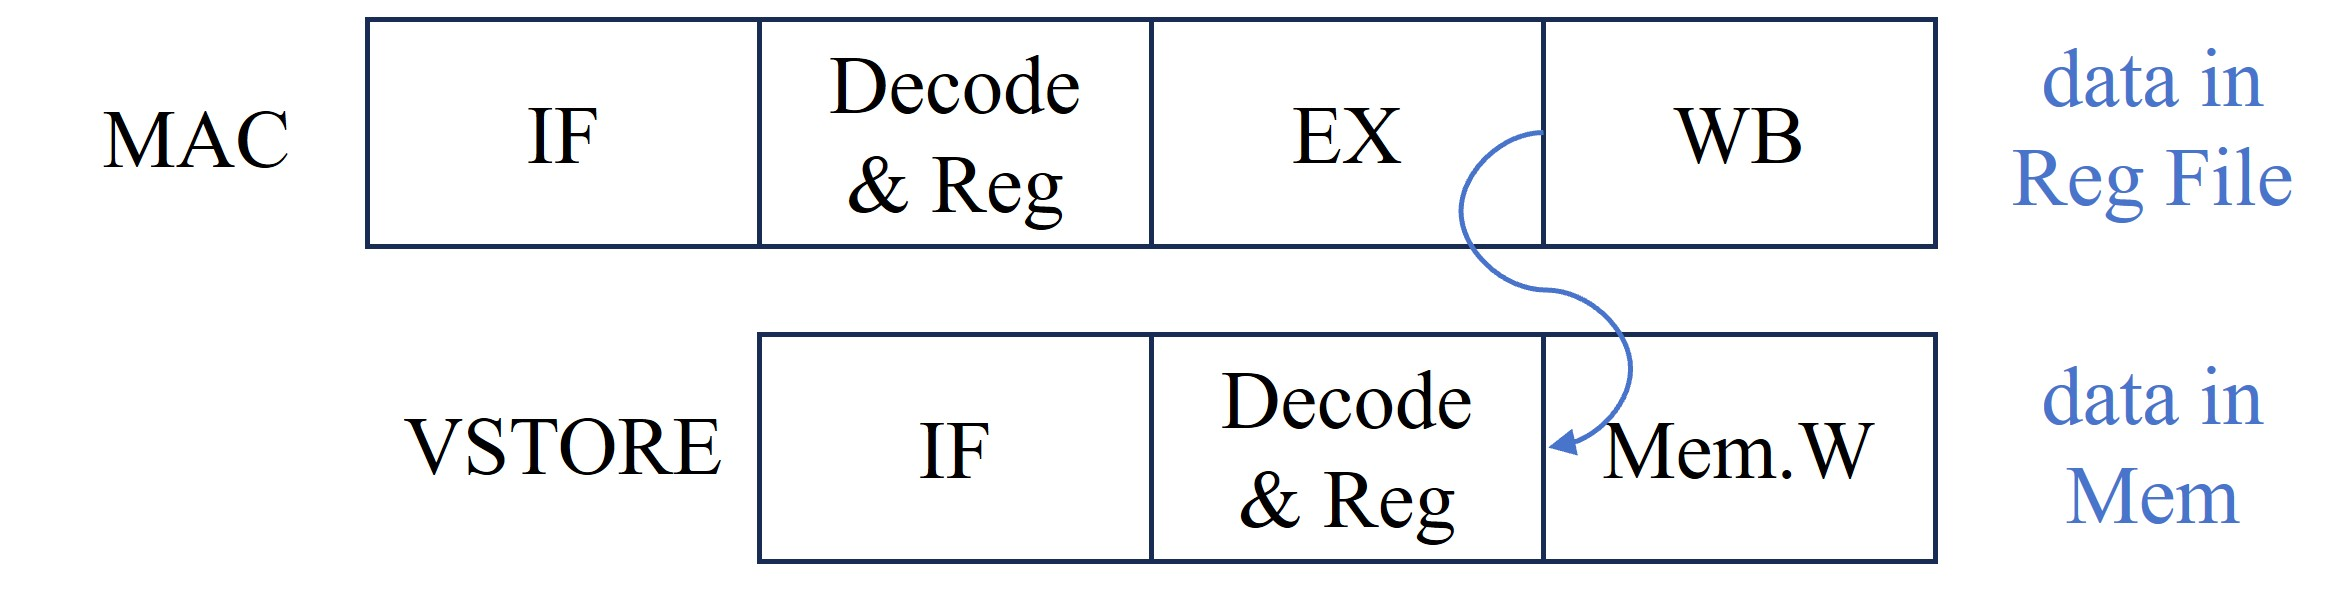
\includegraphics[width=11.1cm]{pic/STORE_RAW3.jpg}}
    \caption{VSTORE指令造成的RAW数据冒险情况}
    \label{Fig.main}
\end{figure}

在实际架构中,为了应对MAC造成的RAW,添加了VLOAD Forward和LOAD Forward数据通路以及相应的数据选择器,分别用于矢量和标量的前馈。为了应对VSTORE造成的前馈,添加了VSTORE Forward数据通路以及相应的数据选择器。
由于位置有限,架构图中没有进一步画出控制信号和每种前馈通路的不同情况,只画出通路的示意图。

\section{设计实现}
\subsection{顶层模块}
顶层模块包括了指令缓存,译码器,立即数生成模块,标量寄存器和矢量寄存器,标量缓存和矢量缓存,乘加单元和控制单元。
在模块内部实现了指令计数器,数据选择器,以及各个模块的连线,按照架构图的模式搭建,使各个模块构成一个完整的VPU。

模块提供了外部交互的接口,分为三种模式,写入、执行和读取。写入模式下,VPU不工作,由外部对指令缓存、标量存储器和向量存储器进行数据写入,
在这个模式下实现了VPU的编程和数据的初始化;
执行模式下,VPU正常工作,从指令缓存逐条读取指令,执行指令并更新寄存器和存储器;
读取模式下,VPU停止工作,外部可以从标量缓存和矢量缓存中读取数据,用于验证计算结果。
具体端口和参数说明如图5所示。

\begin{figure}[htbp]
    \centering
    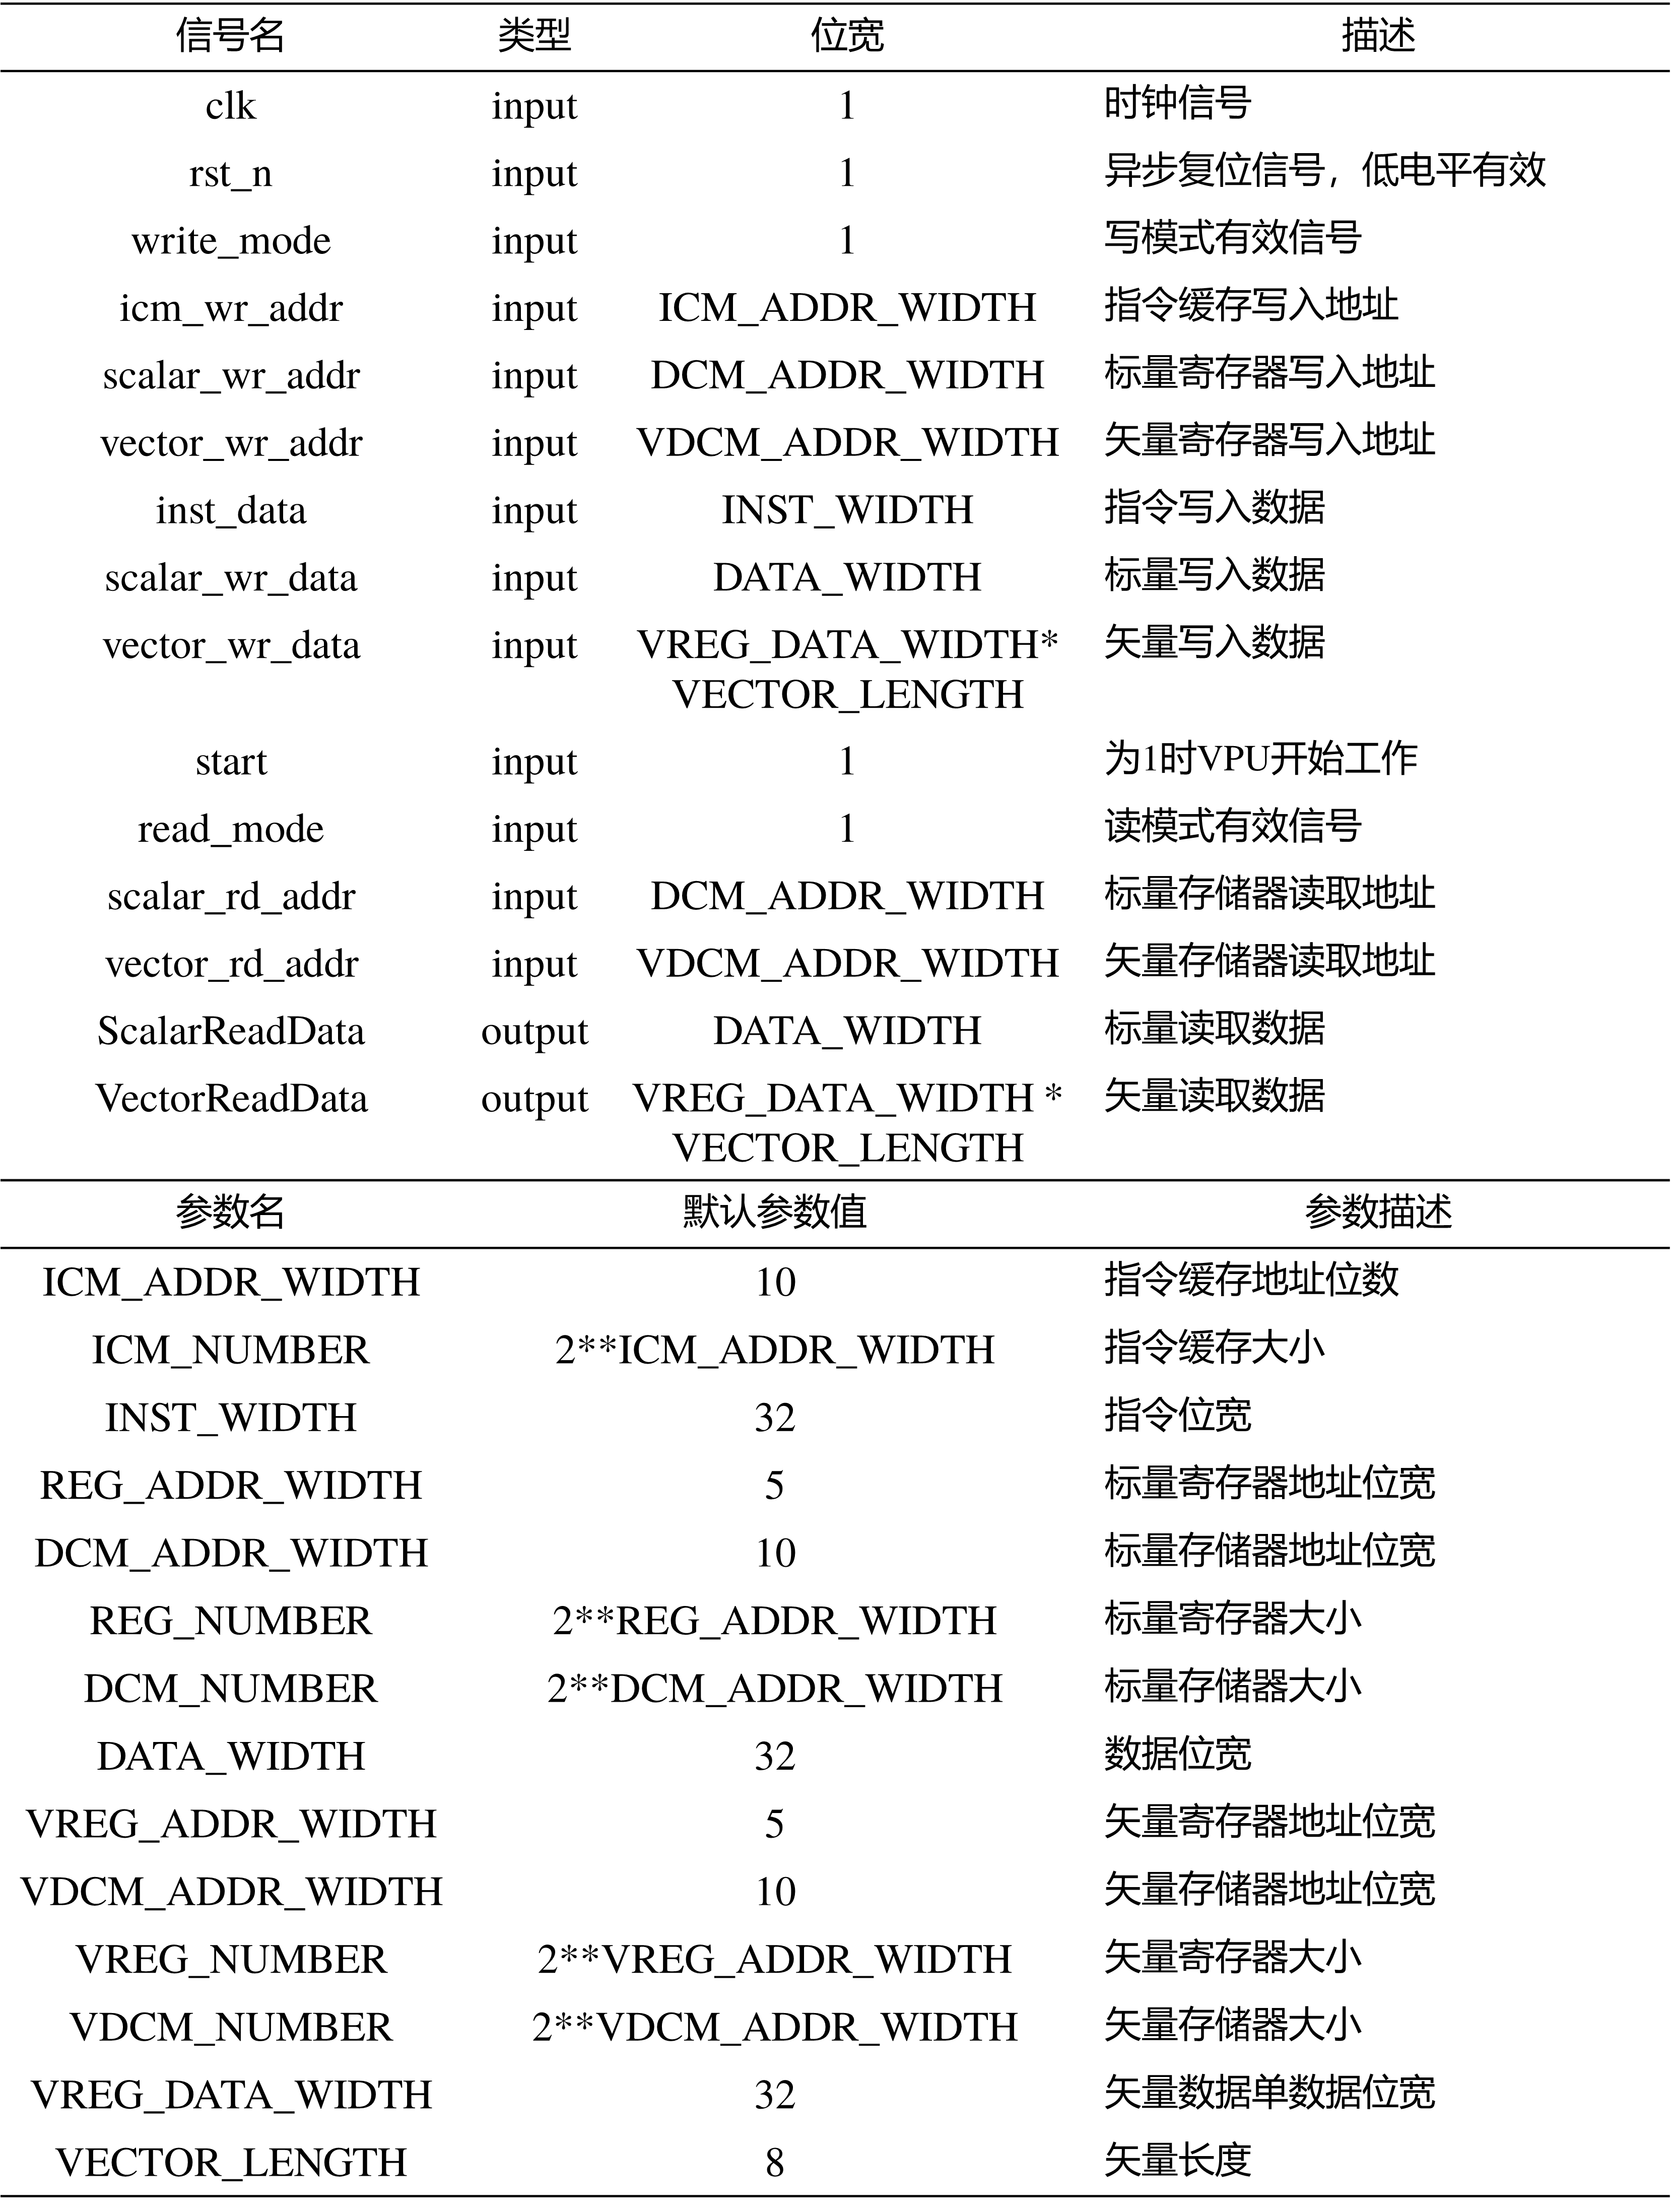
\includegraphics[width=16cm]{pic/VPU.png}
    \caption{顶层模块端口说明}
\end{figure}

\subsection{指令缓存模块}
指令缓存模块有一个写使能信号,有效时接收外部的数据和地址,进行编程。其他时候则根据读地址输出指令。
另外,为了方便测试,指令缓存还有一个初始化文件,在测试开始时对缓存进行初始化。需要注意的是,初始化文件需要是.vmem文件,文件中每一行是一个数据,
且不能有注释,行数必须和缓存大小一致,才能成功初始化。
端口和参数说明如图6所示。

\begin{figure}[htbp]
    \centering
    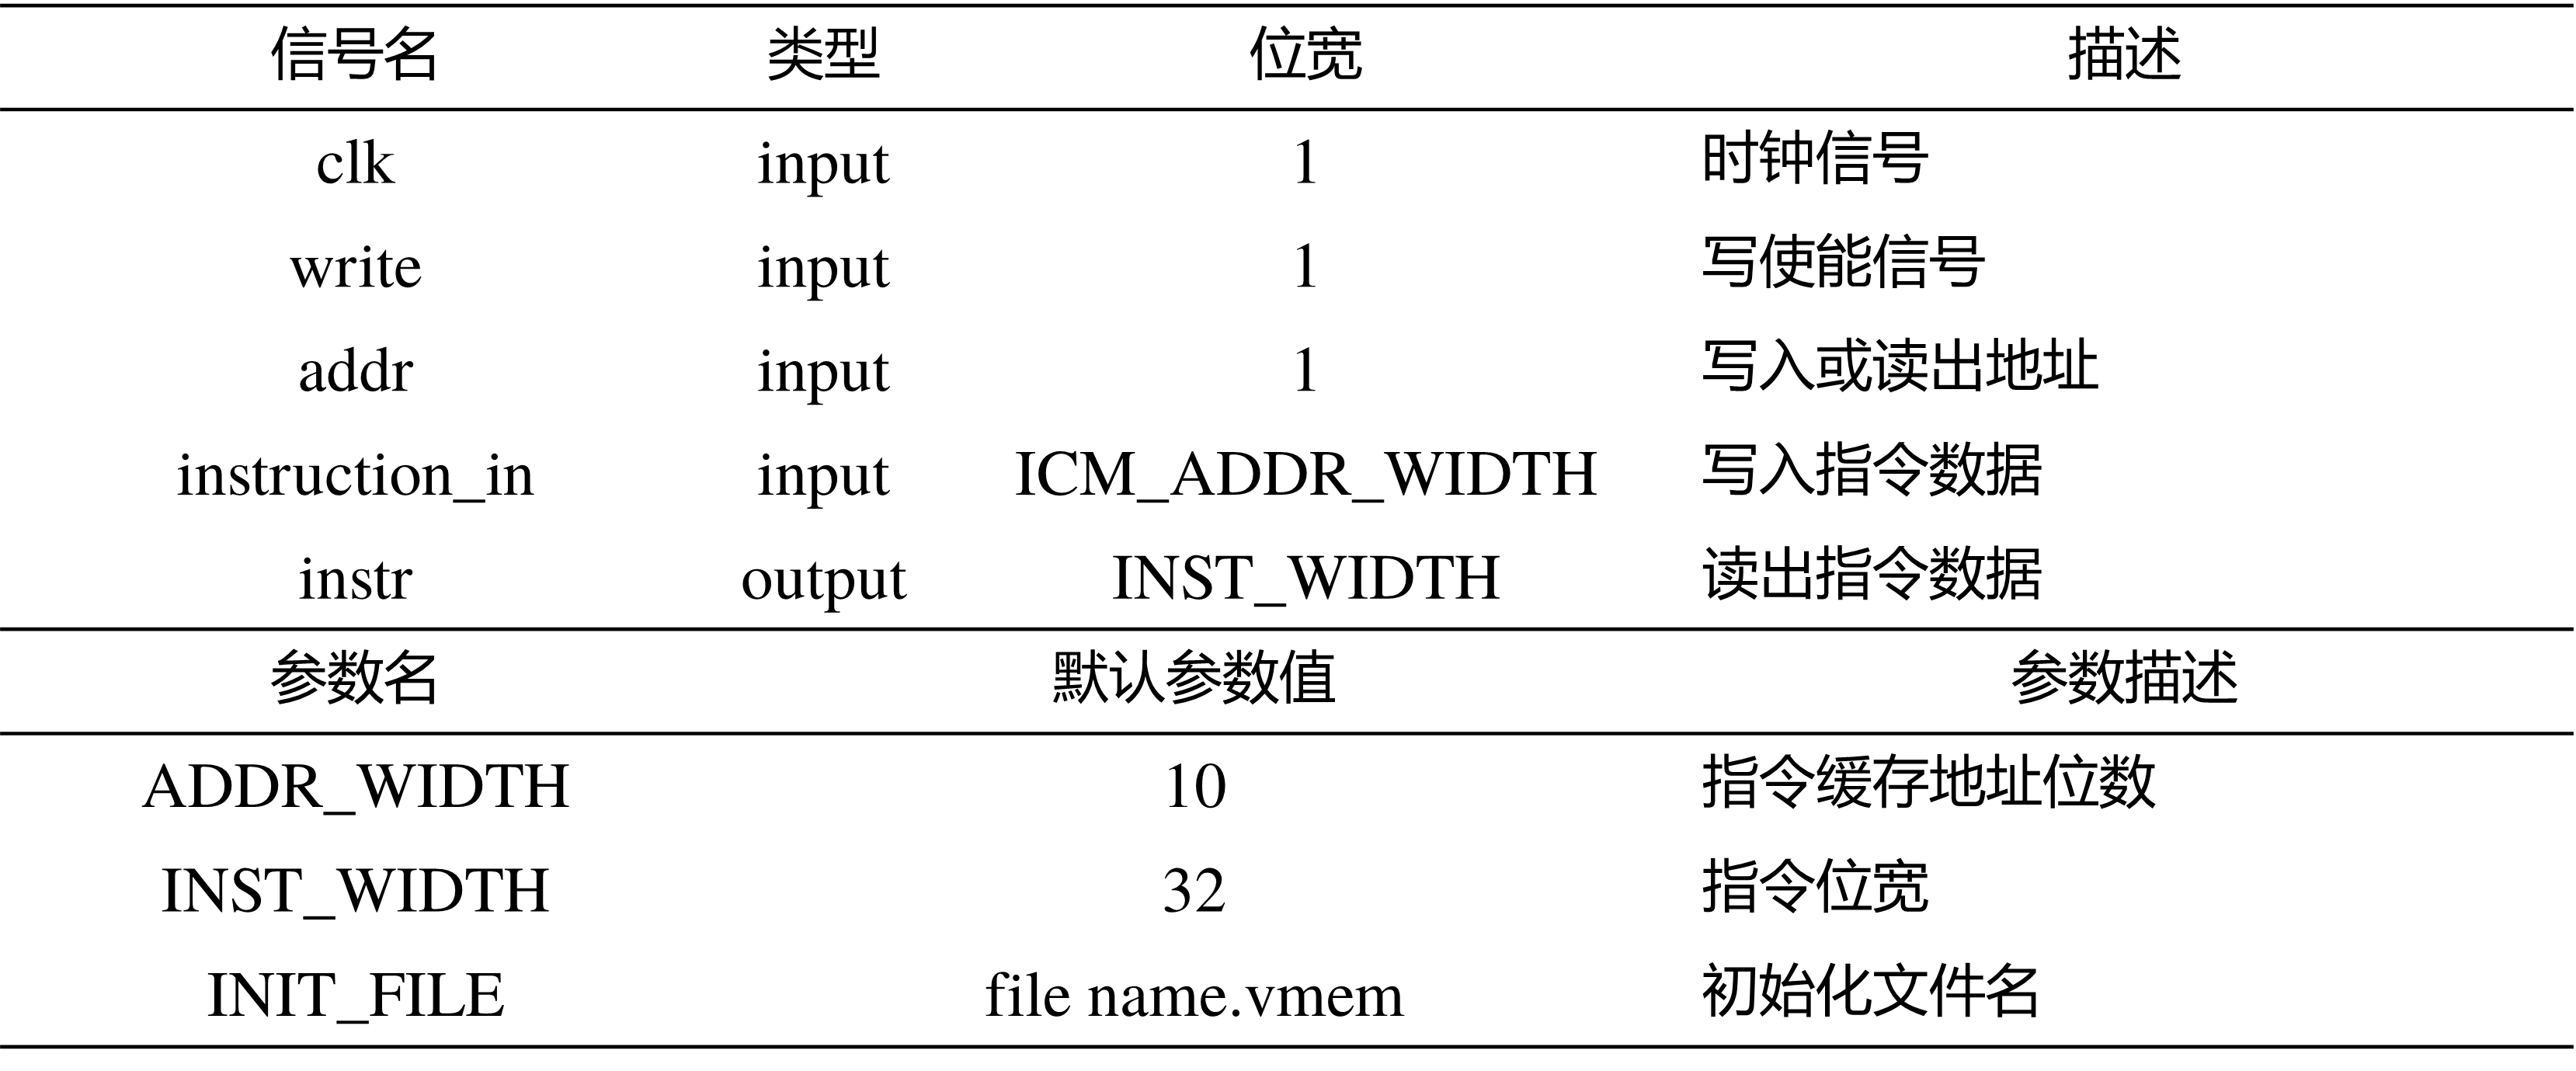
\includegraphics[width=16cm]{pic/ICM.png}
    \caption{指令缓存模块端口说明}
\end{figure}

\subsection{译码器}
译码器模块接收指令缓存输出的指令,判断指令类型并解码为立即数和寄存器地址等信息,输出给其他模块。端口和参数说明如图7所示。

\begin{figure}[htbp]
    \centering
    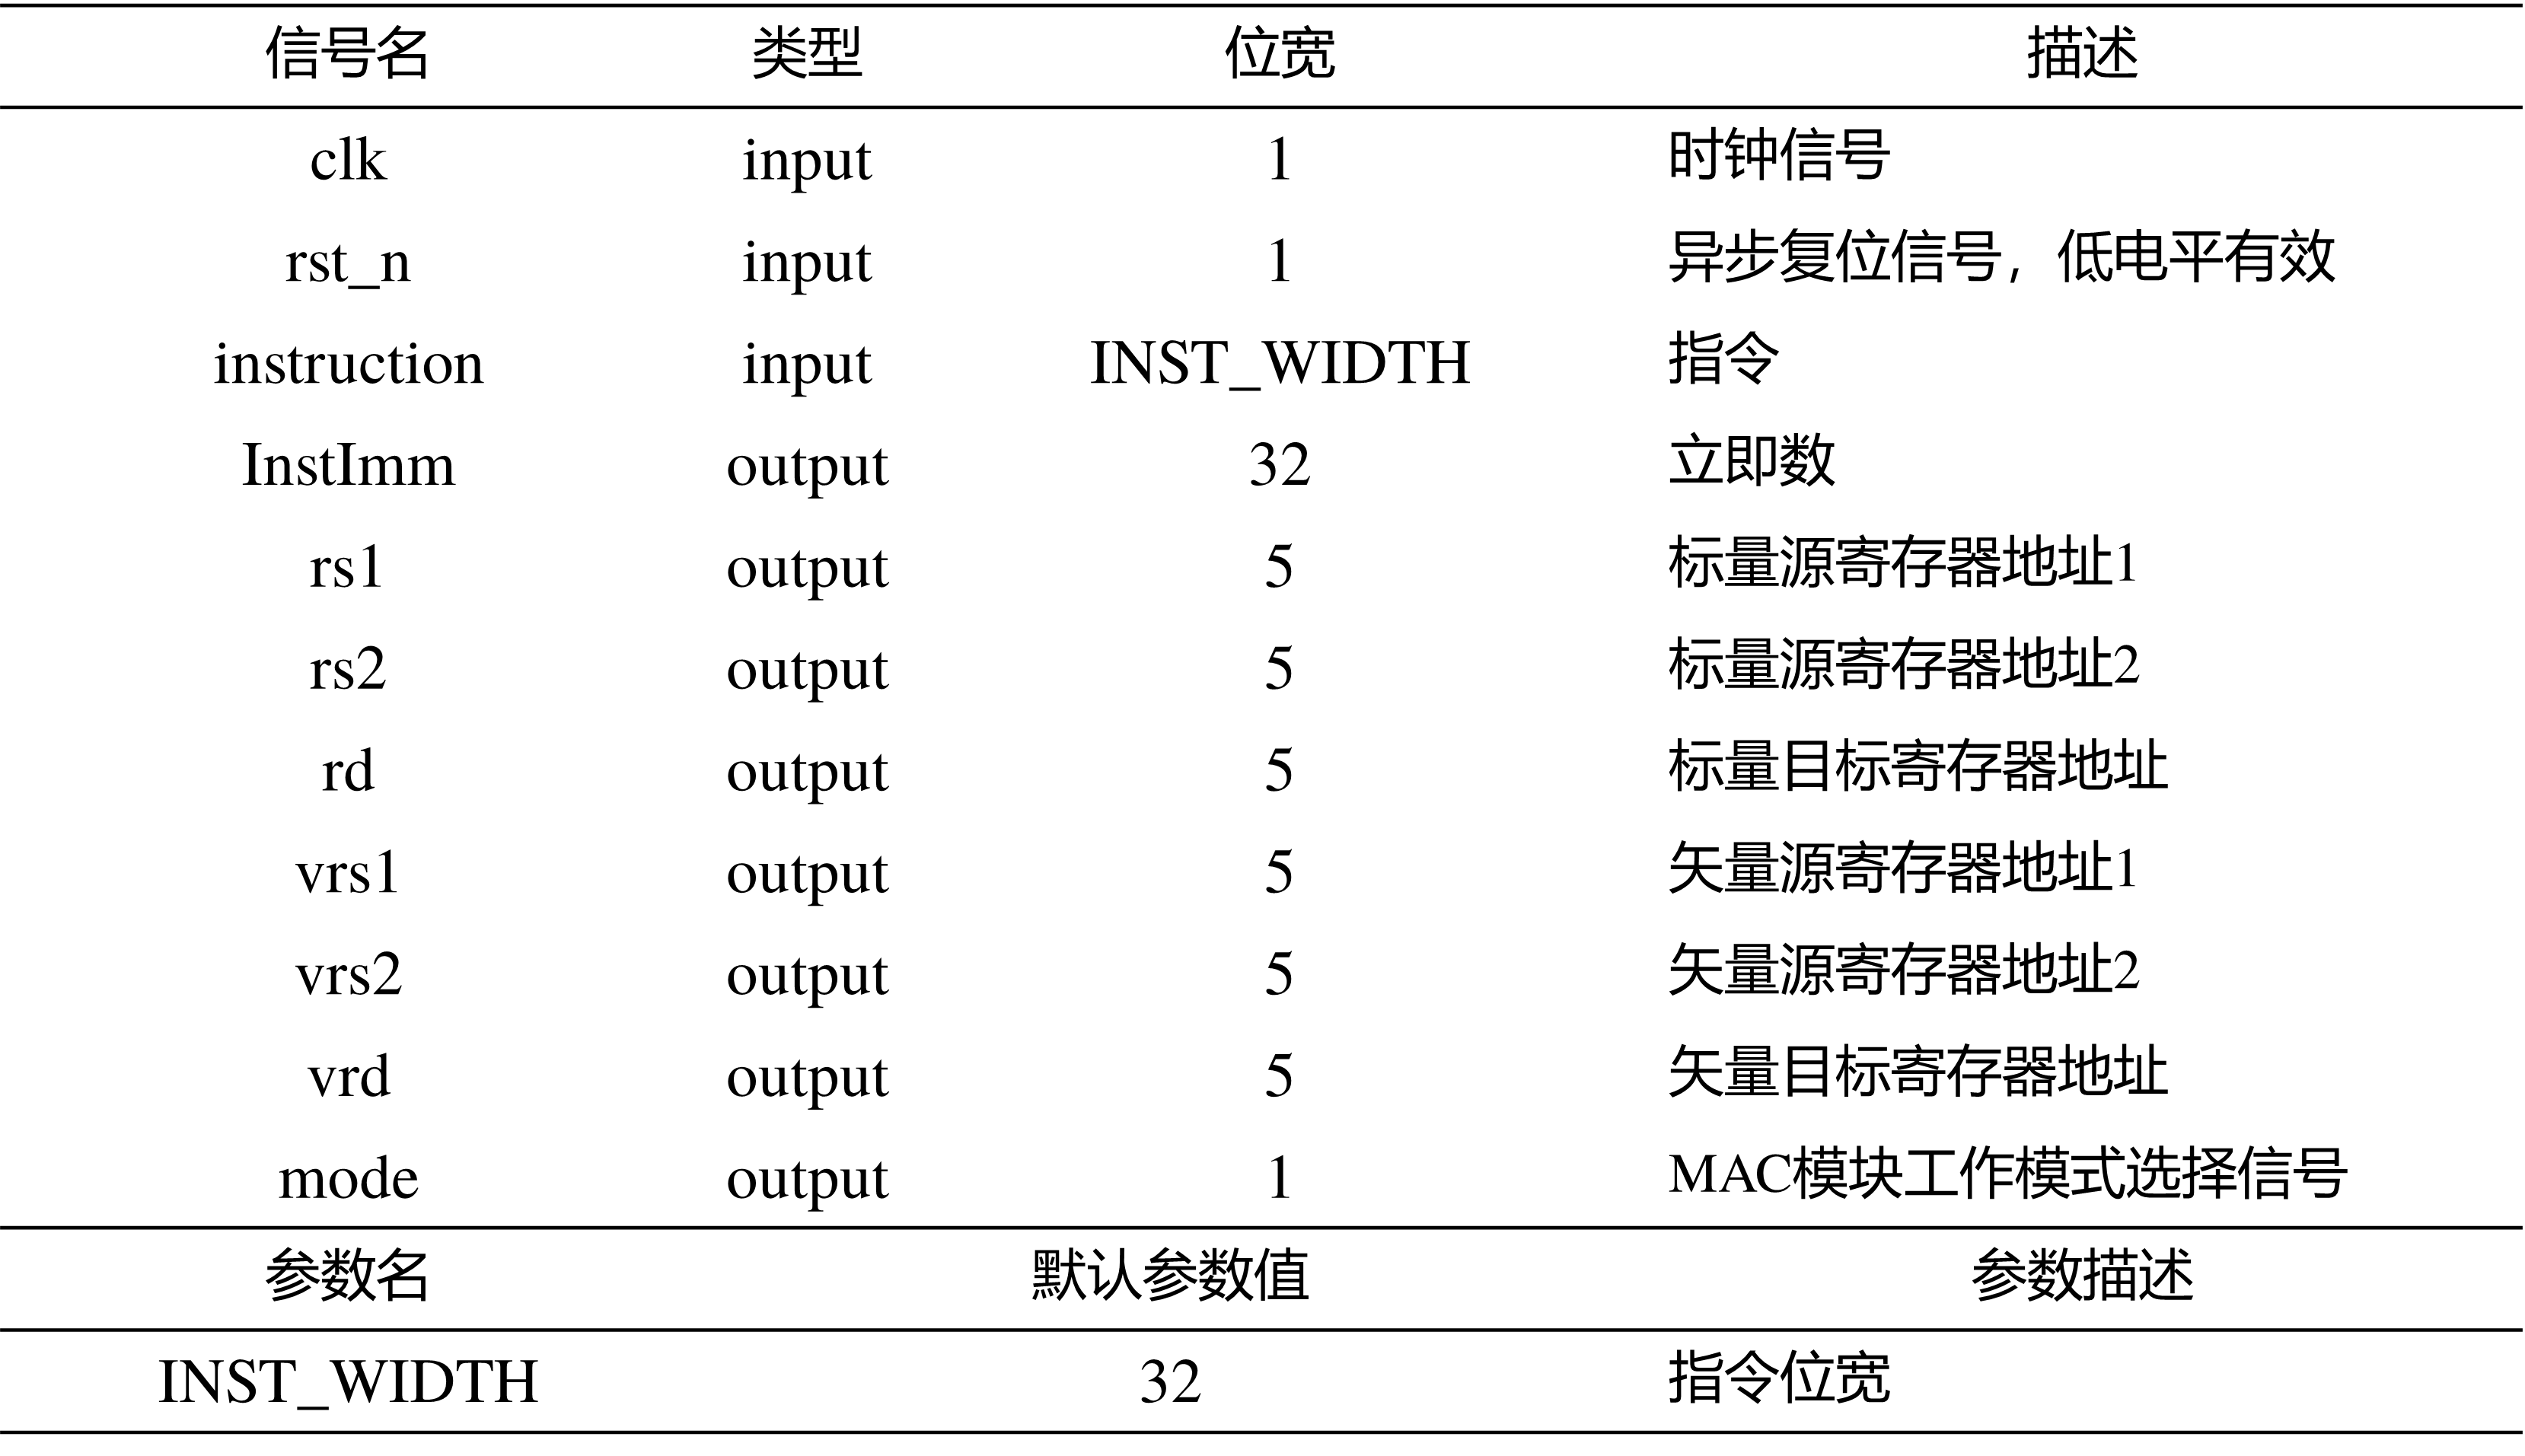
\includegraphics[width=16cm]{pic/Decode.png}
    \caption{译码器模块端口说明}
\end{figure}

\subsection{立即数生成模块}

立即数生成模块接收译码器输出的指令,经过一个周期后生成立即数。主要目的是流水线的时序对齐。端口和参数说明如图8所示。

\begin{figure}[htbp]
    \centering
    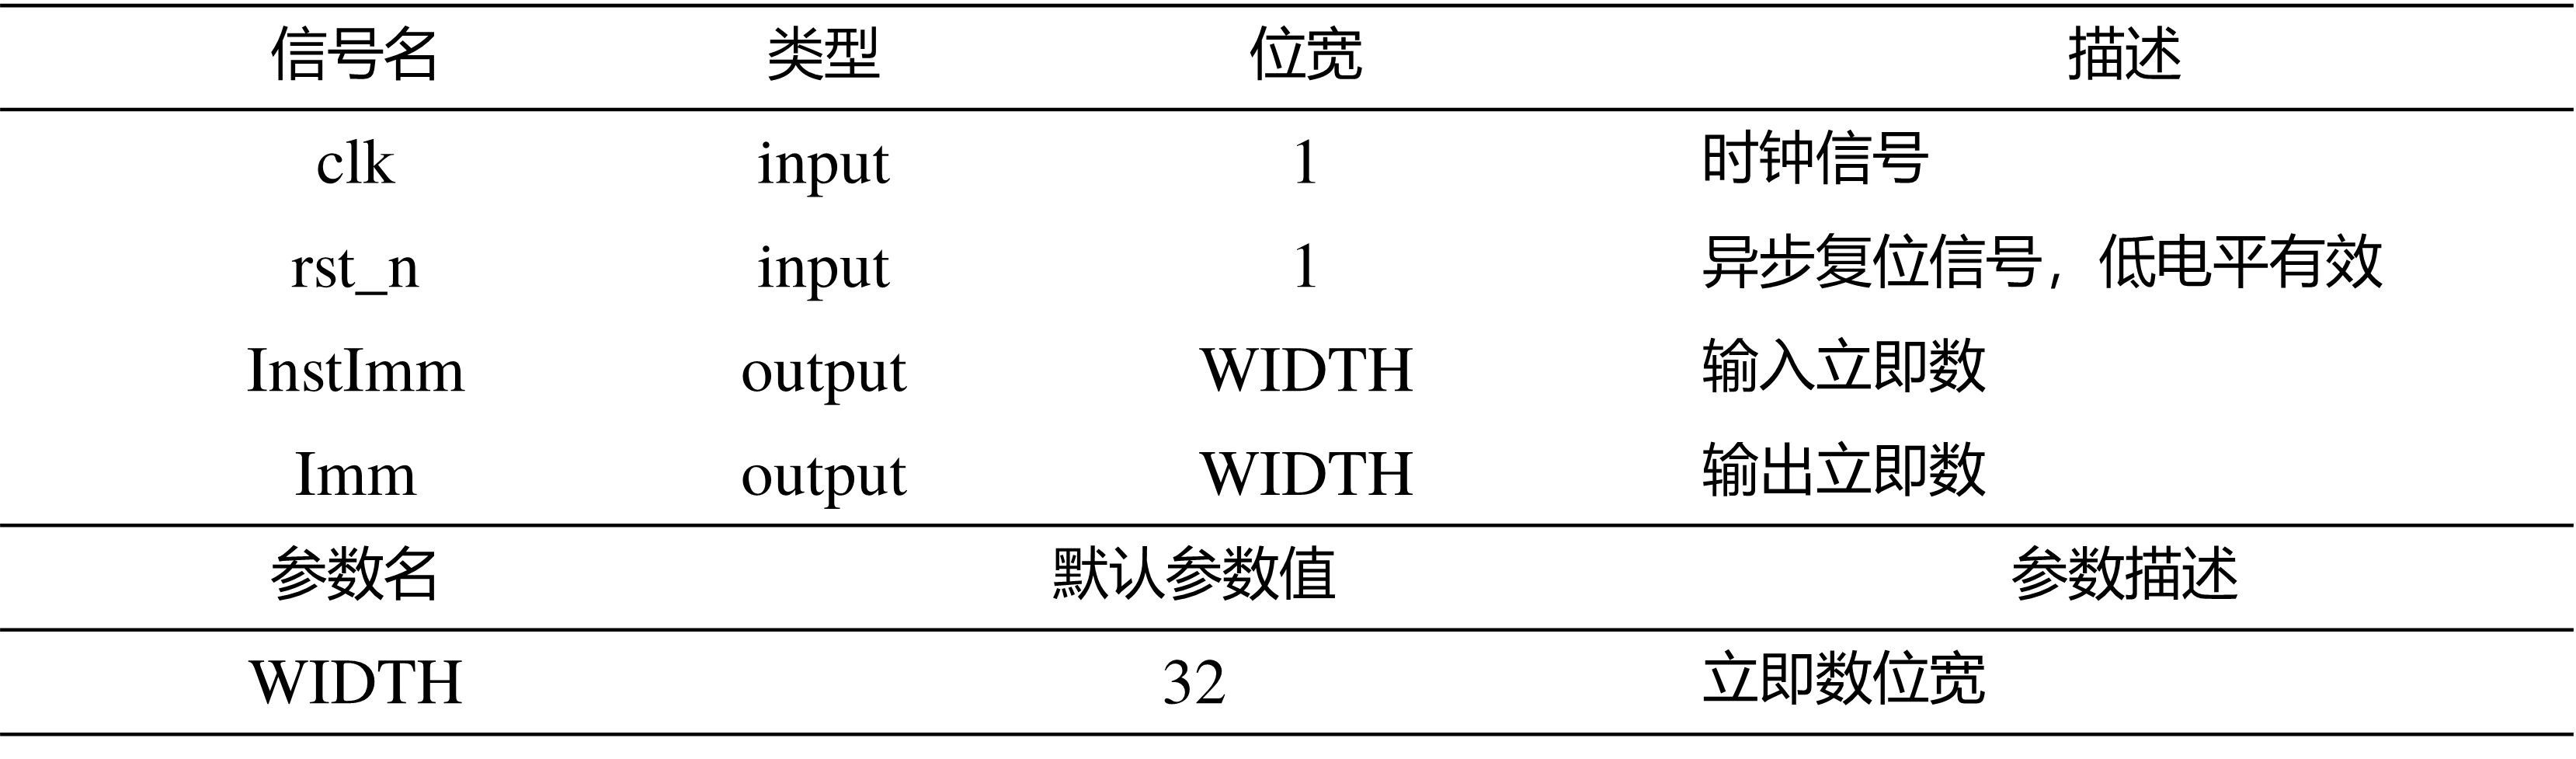
\includegraphics[width=16cm]{pic/Immgen.png}
    \caption{立即数生成模块端口说明}
\end{figure}

\subsection{标量寄存器}
标量寄存器是一个三端口模块,有两组读地址和数据接口,一组写地址和数据接口。读数据没有设置使能信号,默认始终根据读地址输出数据,
写入数据需要写使能信号有效时才写入数据。端口和参数说明如图9所示。

\begin{figure}[htbp]
    \centering
    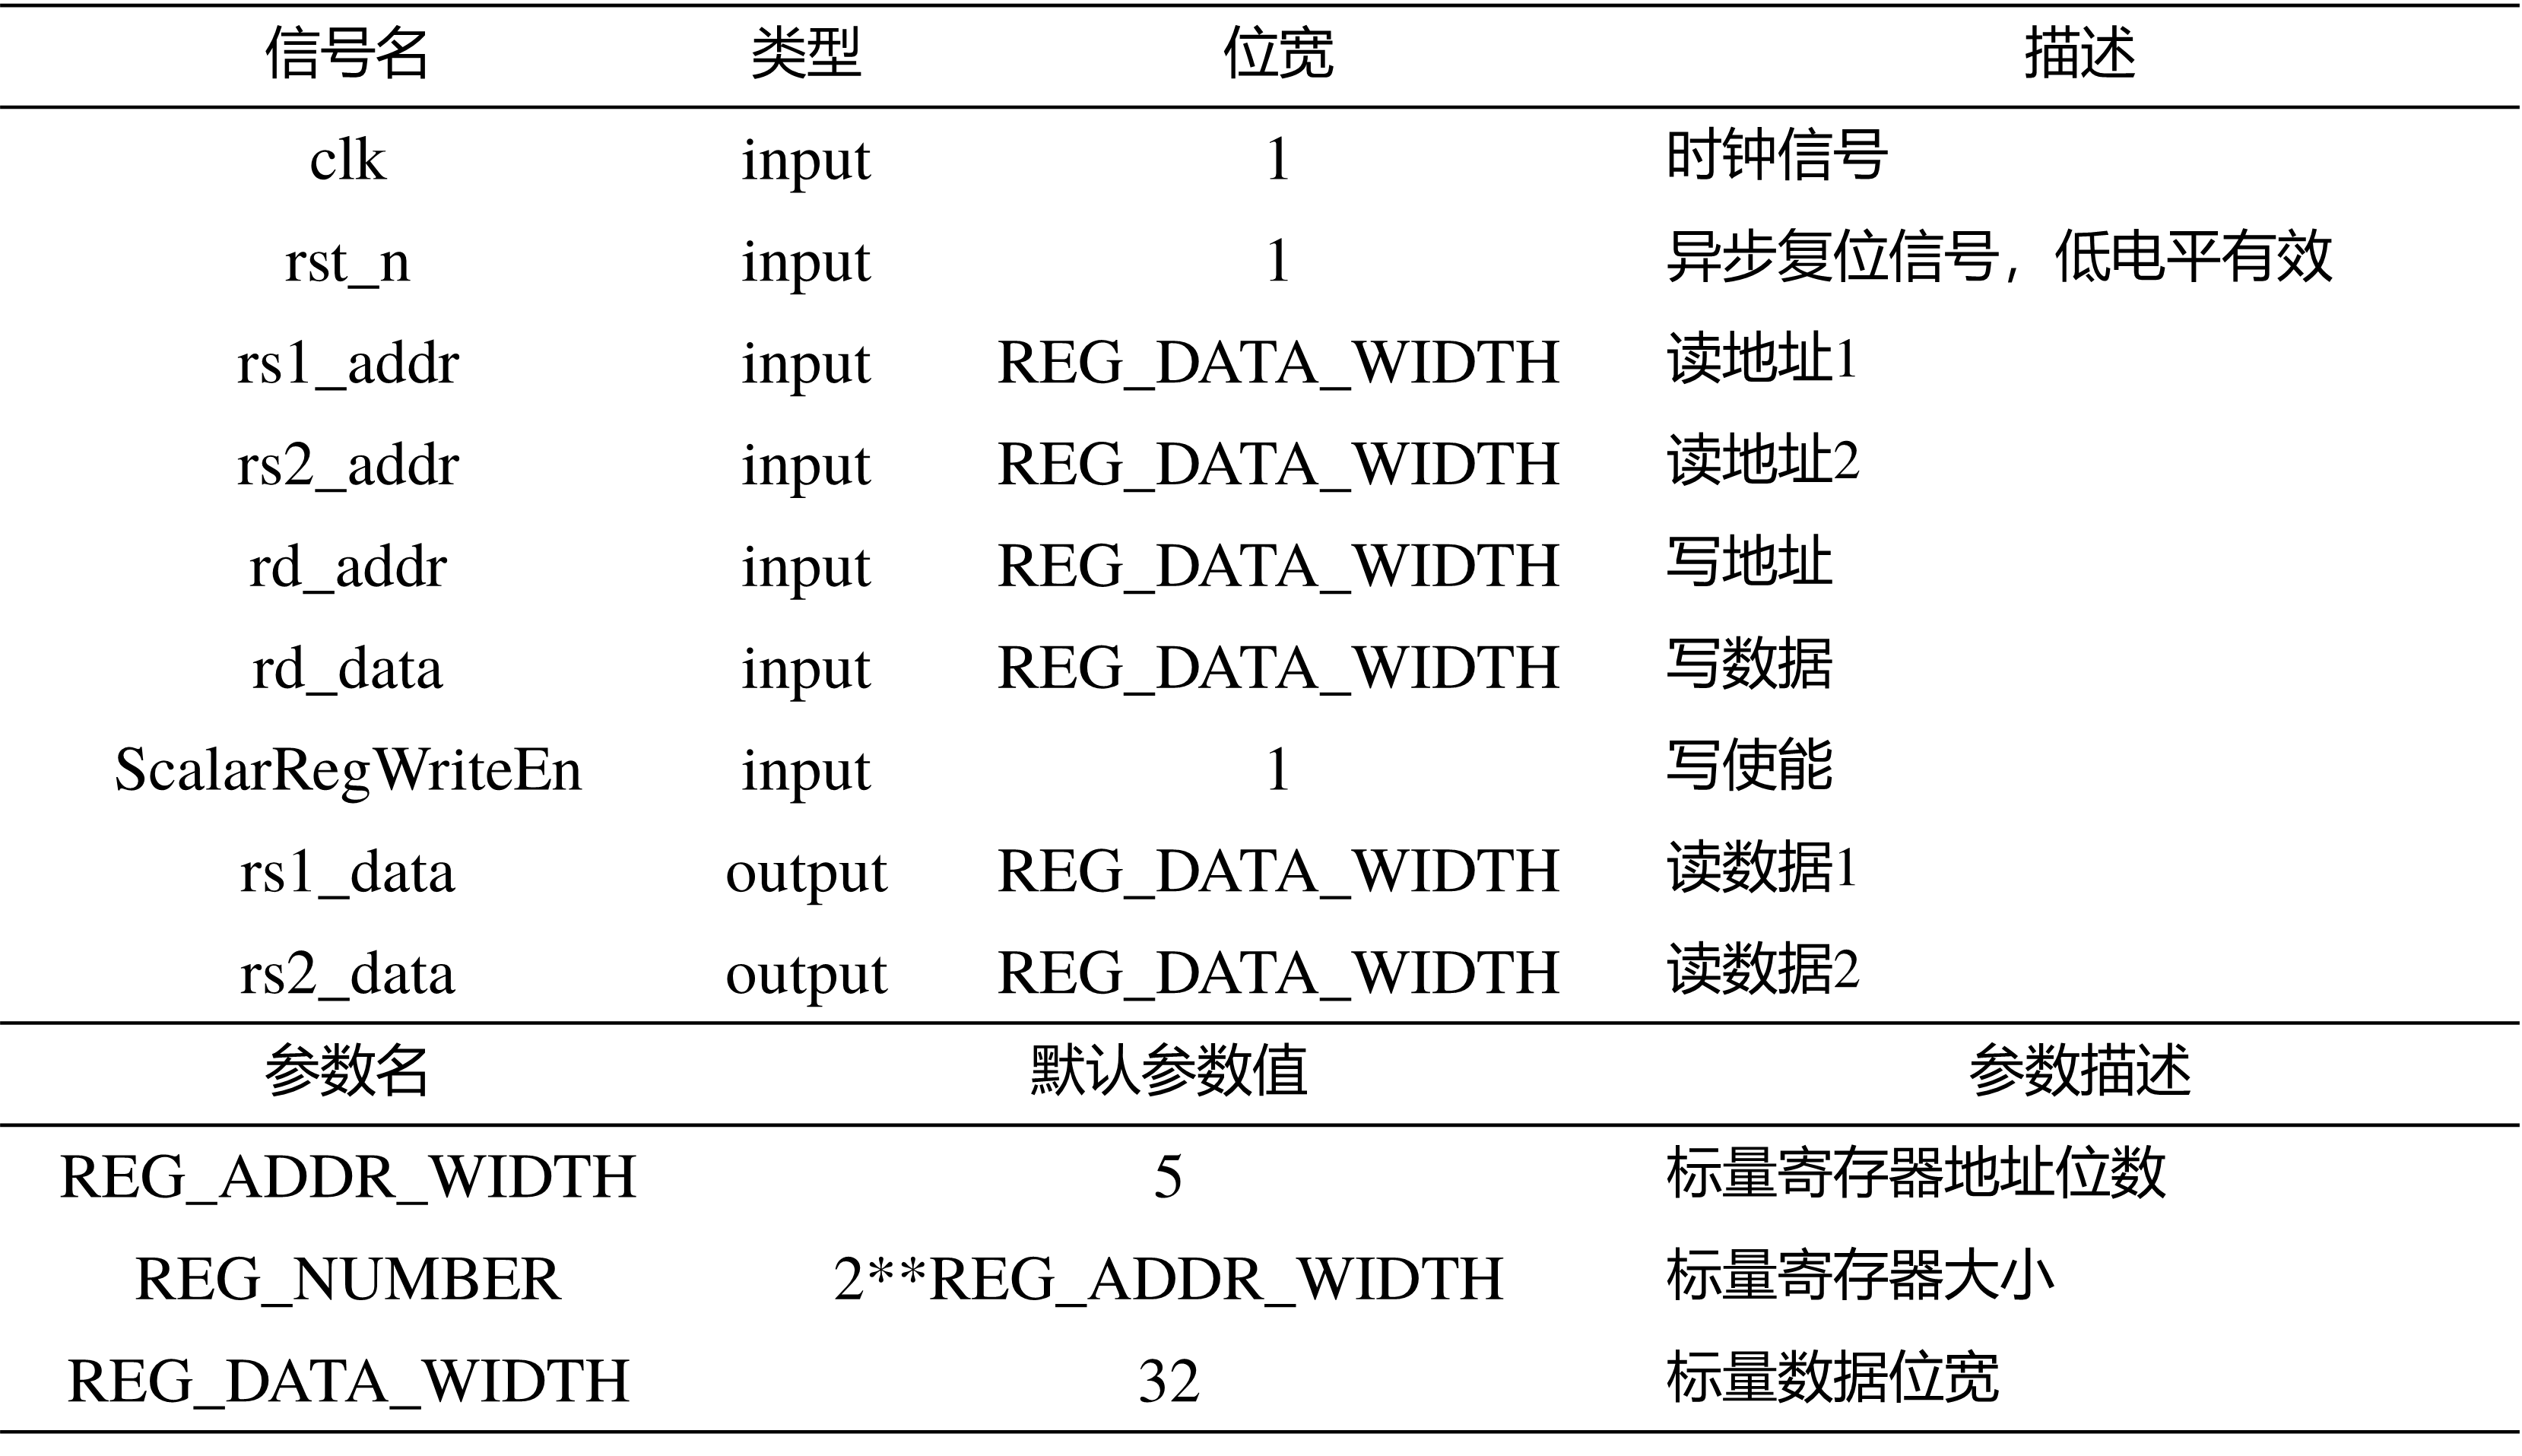
\includegraphics[width=16cm]{pic/ScalarRF.png}
    \caption{标量寄存器端口说明}
\end{figure}

\subsection{标量存储器}

标量存储器有一个写端口和一个读端口,根据写使能和读使能决定是否写入数据或读出数据,写入和读出共用一个地址信号。
端口和参数说明如图10所示。

\begin{figure}[htbp]
    \centering
    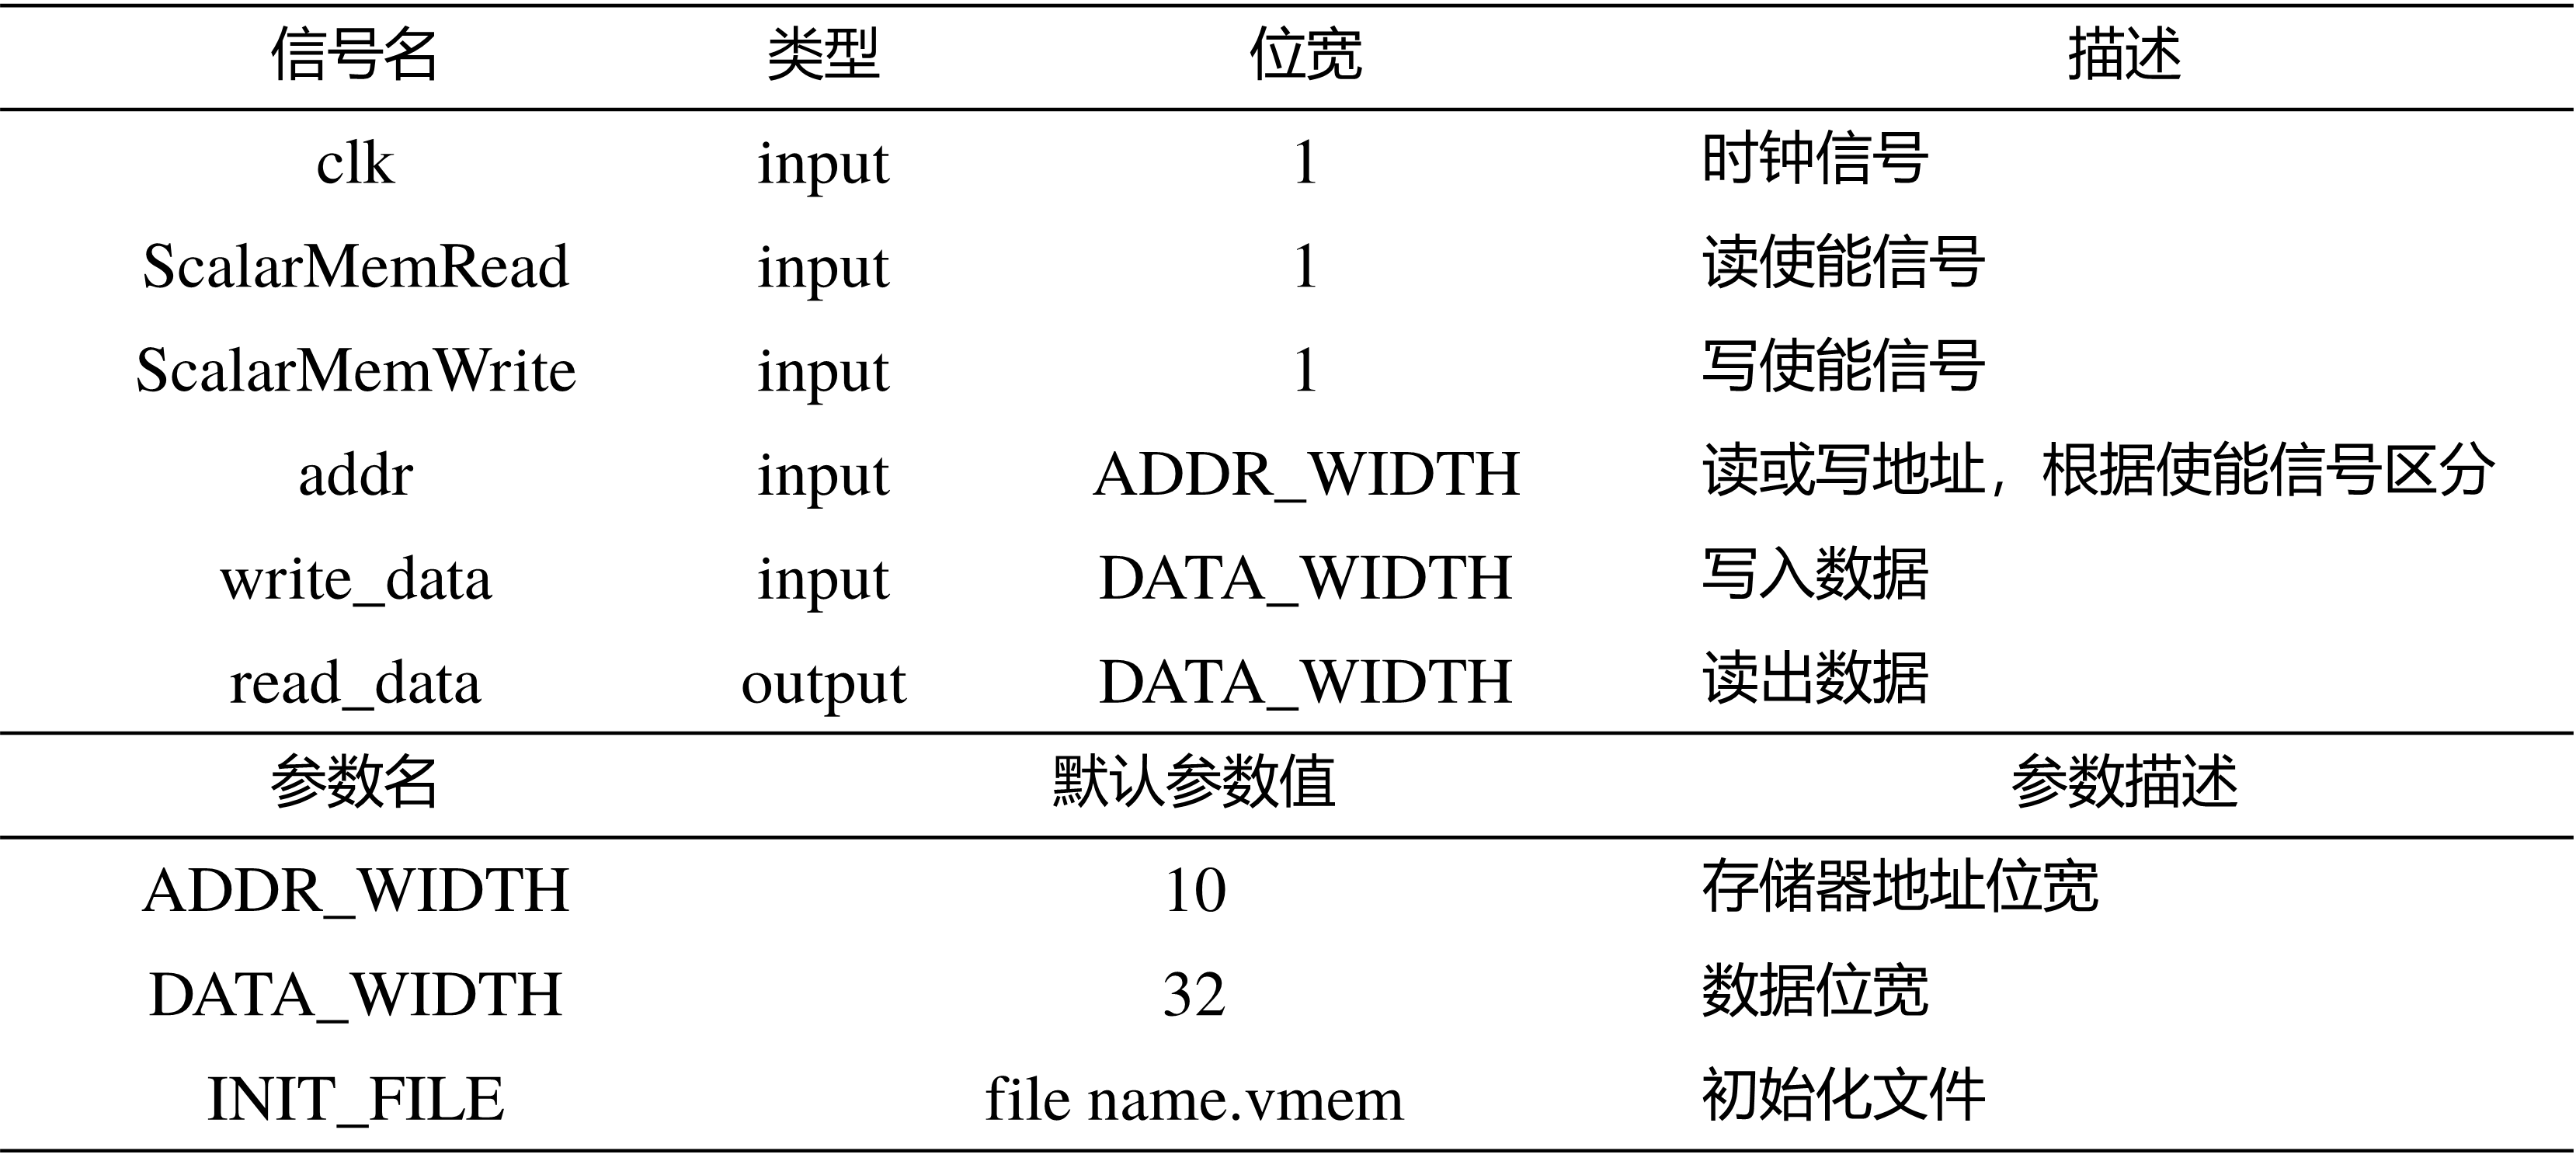
\includegraphics[width=16cm]{pic/ScalarDCM.png}
    \caption{标量存储器端口说明}
\end{figure}

\subsection{矢量寄存器}

矢量寄存器和标量寄存器的功能类似,矢量寄存器的数据位宽更大,每个地址对应一个矢量数据。
端口和参数说明如图11所示。

\begin{figure}[htbp]
    \centering
    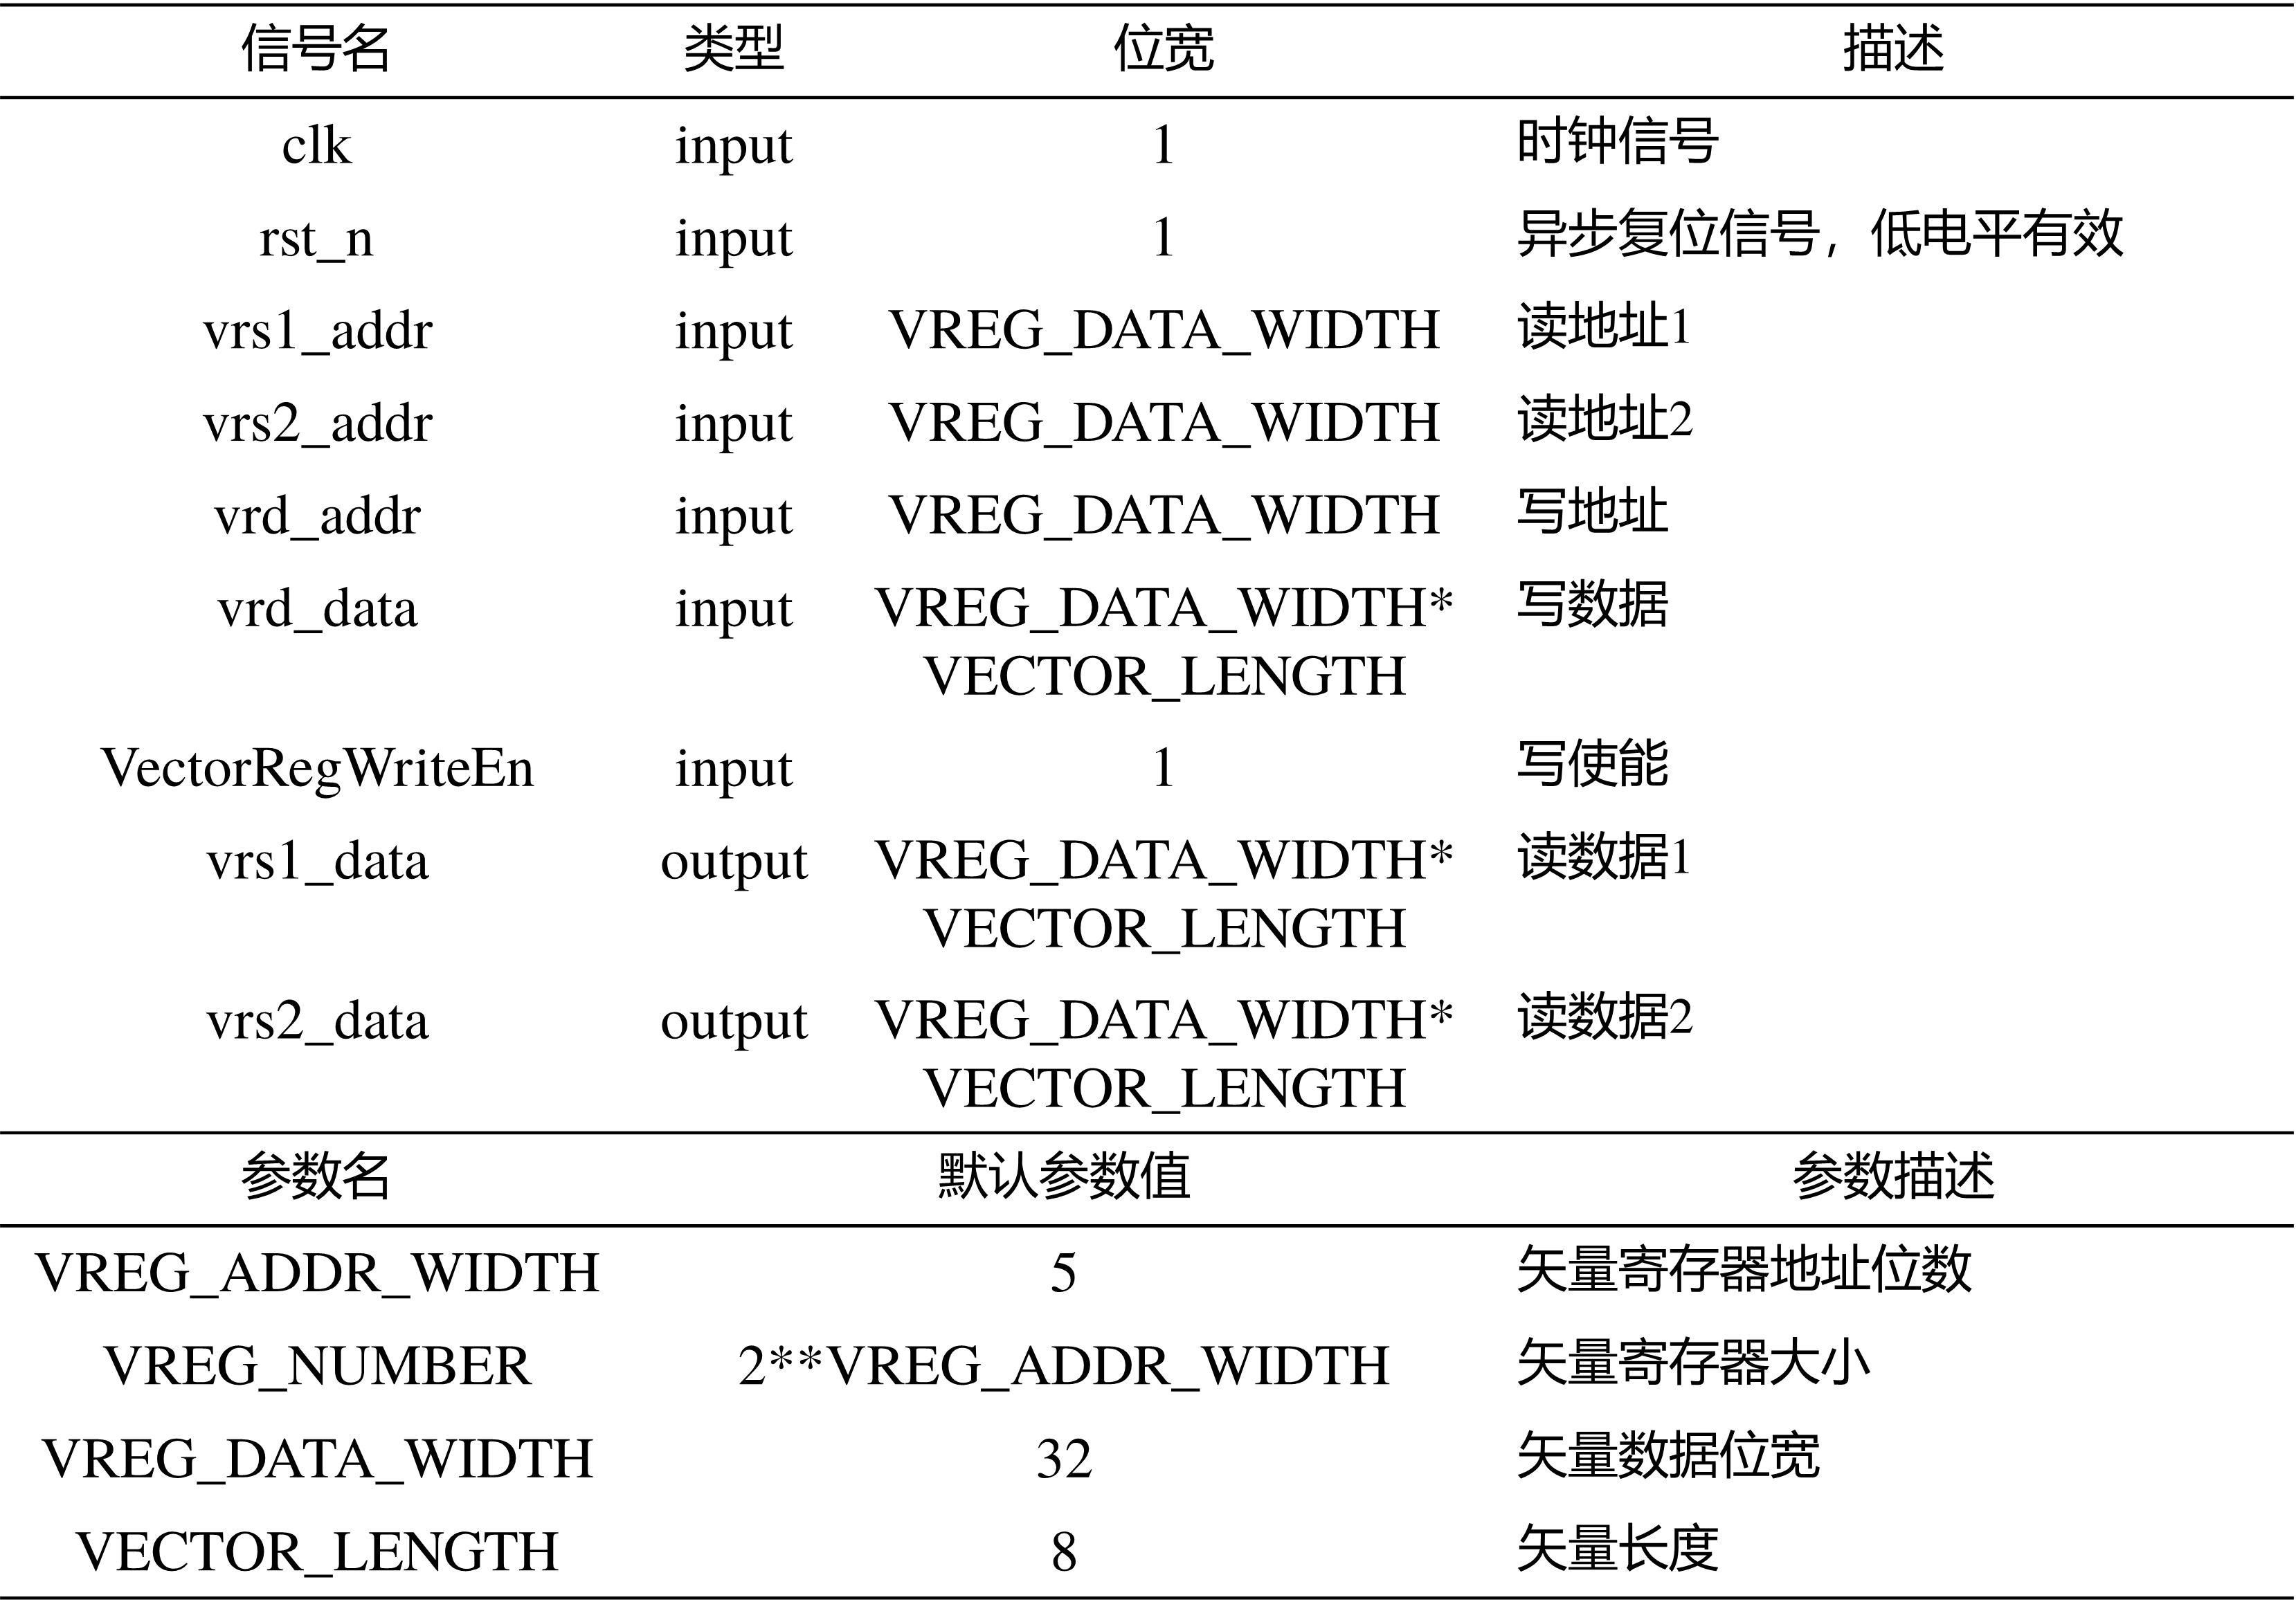
\includegraphics[width=16cm]{pic/VectorRF.png}
    \caption{矢量寄存器端口说明}
\end{figure}

\subsection{矢量存储器}

矢量存储器和标量存储器类似,不同的是矢量存储器的数据位宽更大,每个地址对应一个矢量数据。端口和参数说明如图12所示。

\begin{figure}[htbp]
    \centering
    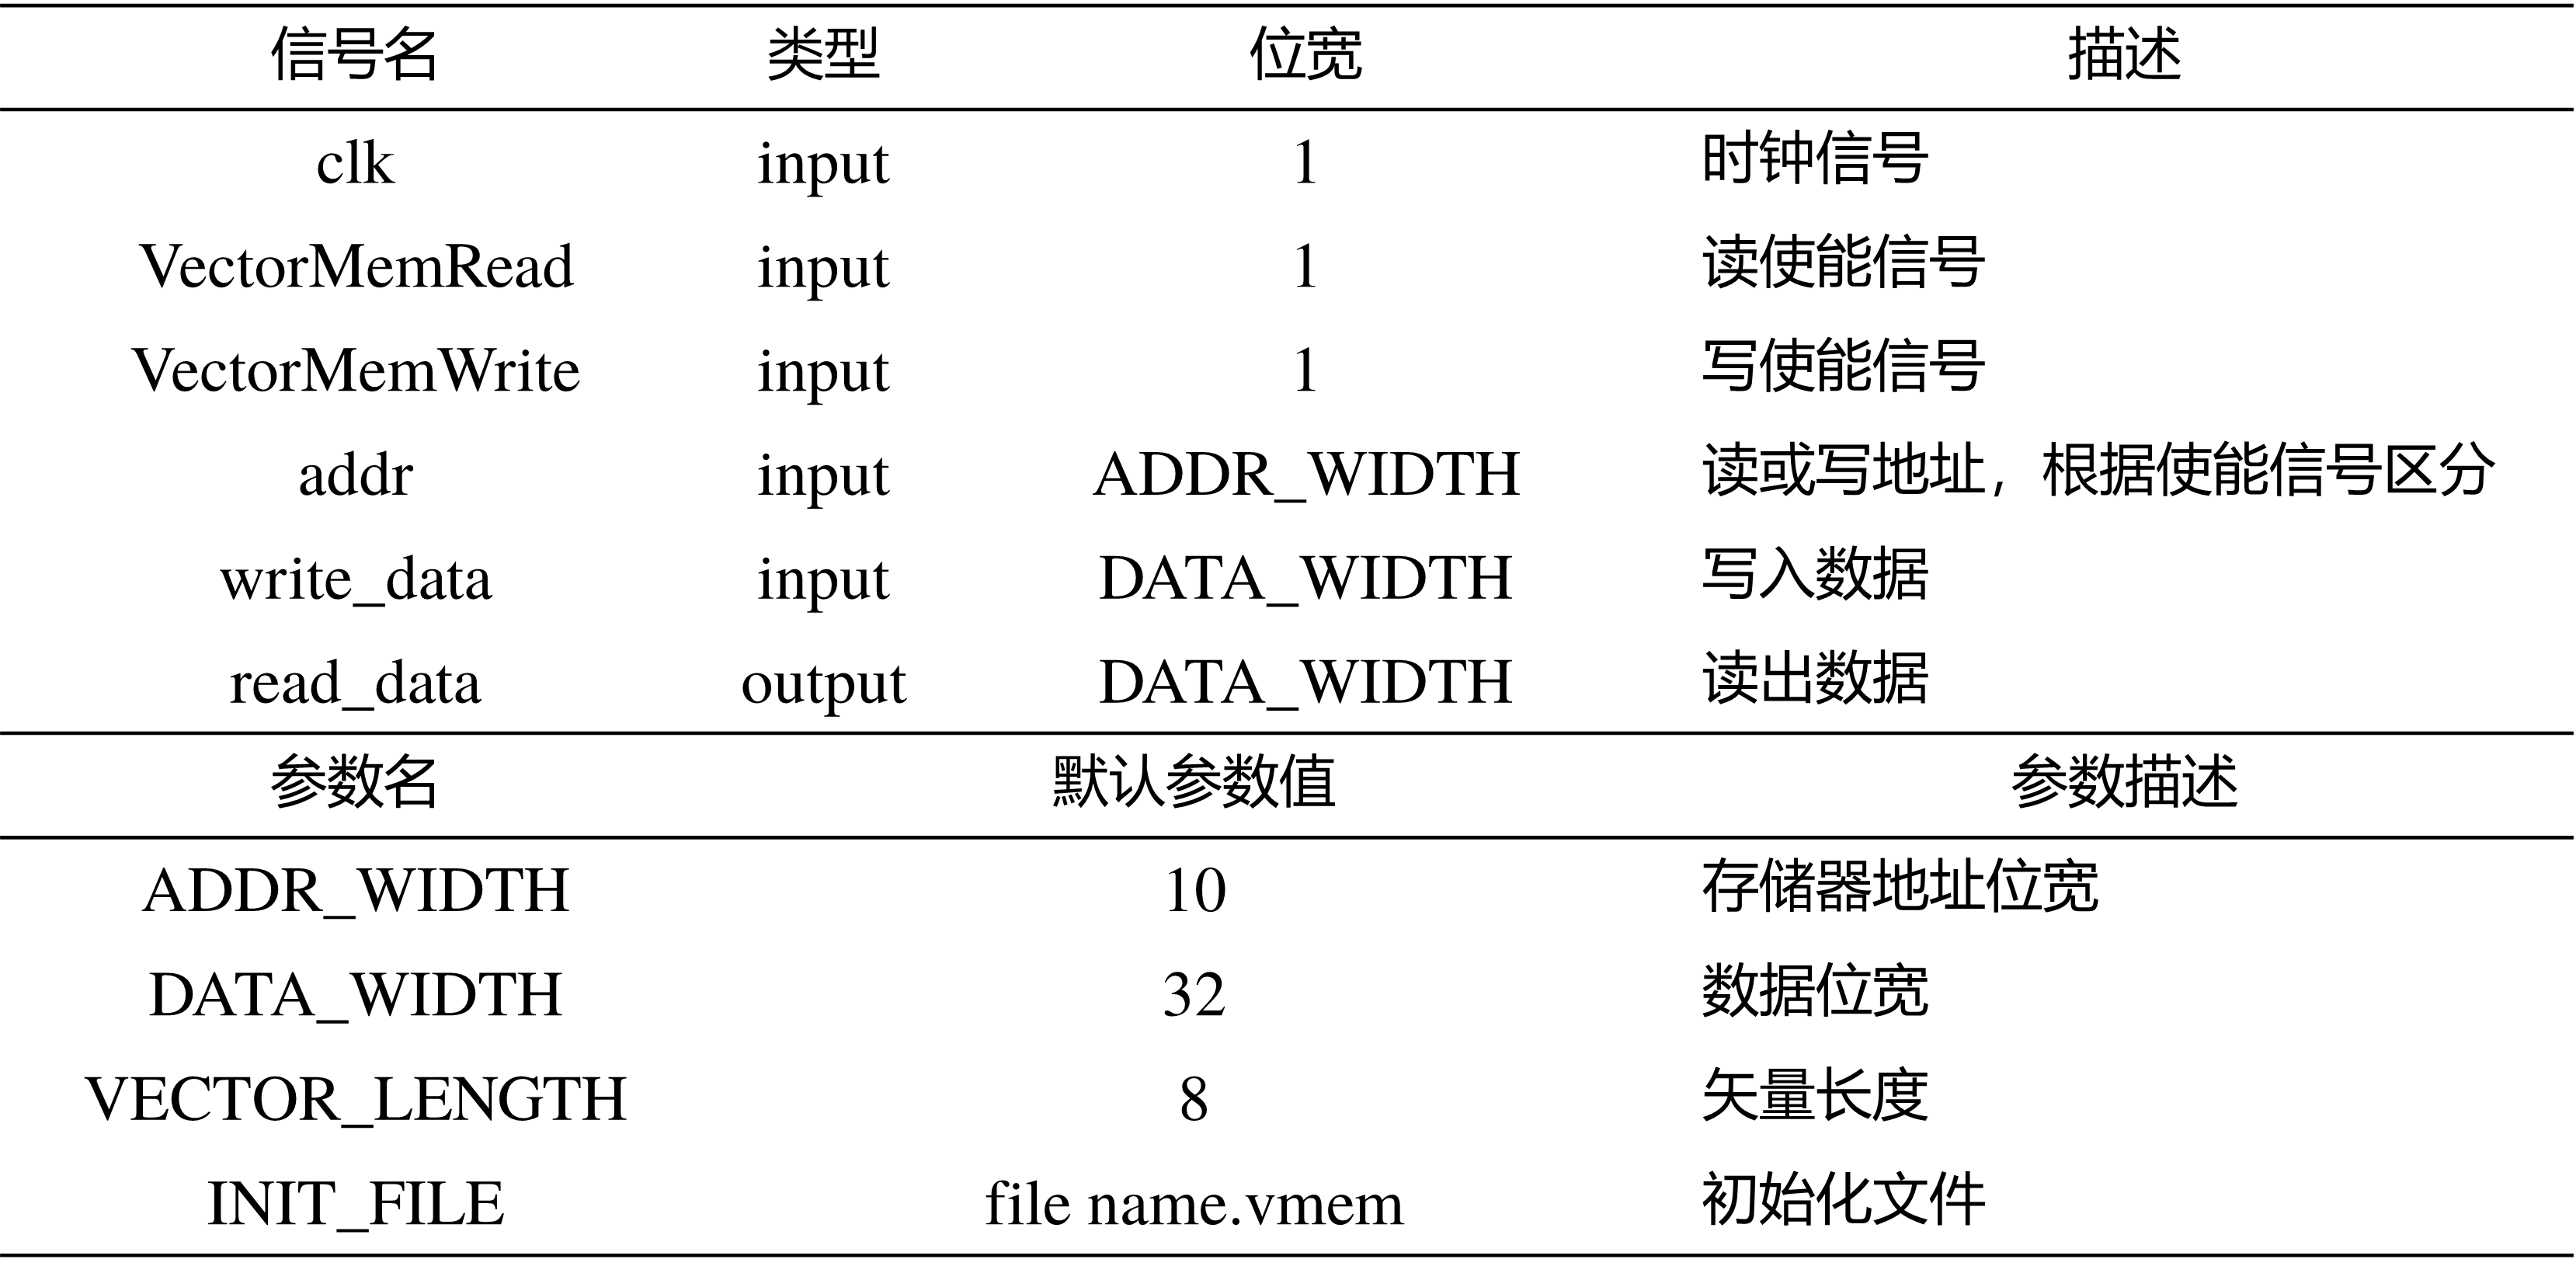
\includegraphics[width=16cm]{pic/VectorDCM.png}
    \caption{矢量存储器端口说明}
\end{figure}

\subsection{标量矢量乘加单元}

MAC模块接收两个矢量和一个标量作为运算输入,根据运算模式输出计算结果。运算模式为1时为初始化,直接将第一个矢量作为输出。
运算模式为0时将第一个矢量乘以标量后加上第二个矢量作为运算结果输出。端口和参数说明如图13所示。

\begin{figure}[htbp]
    \centering
    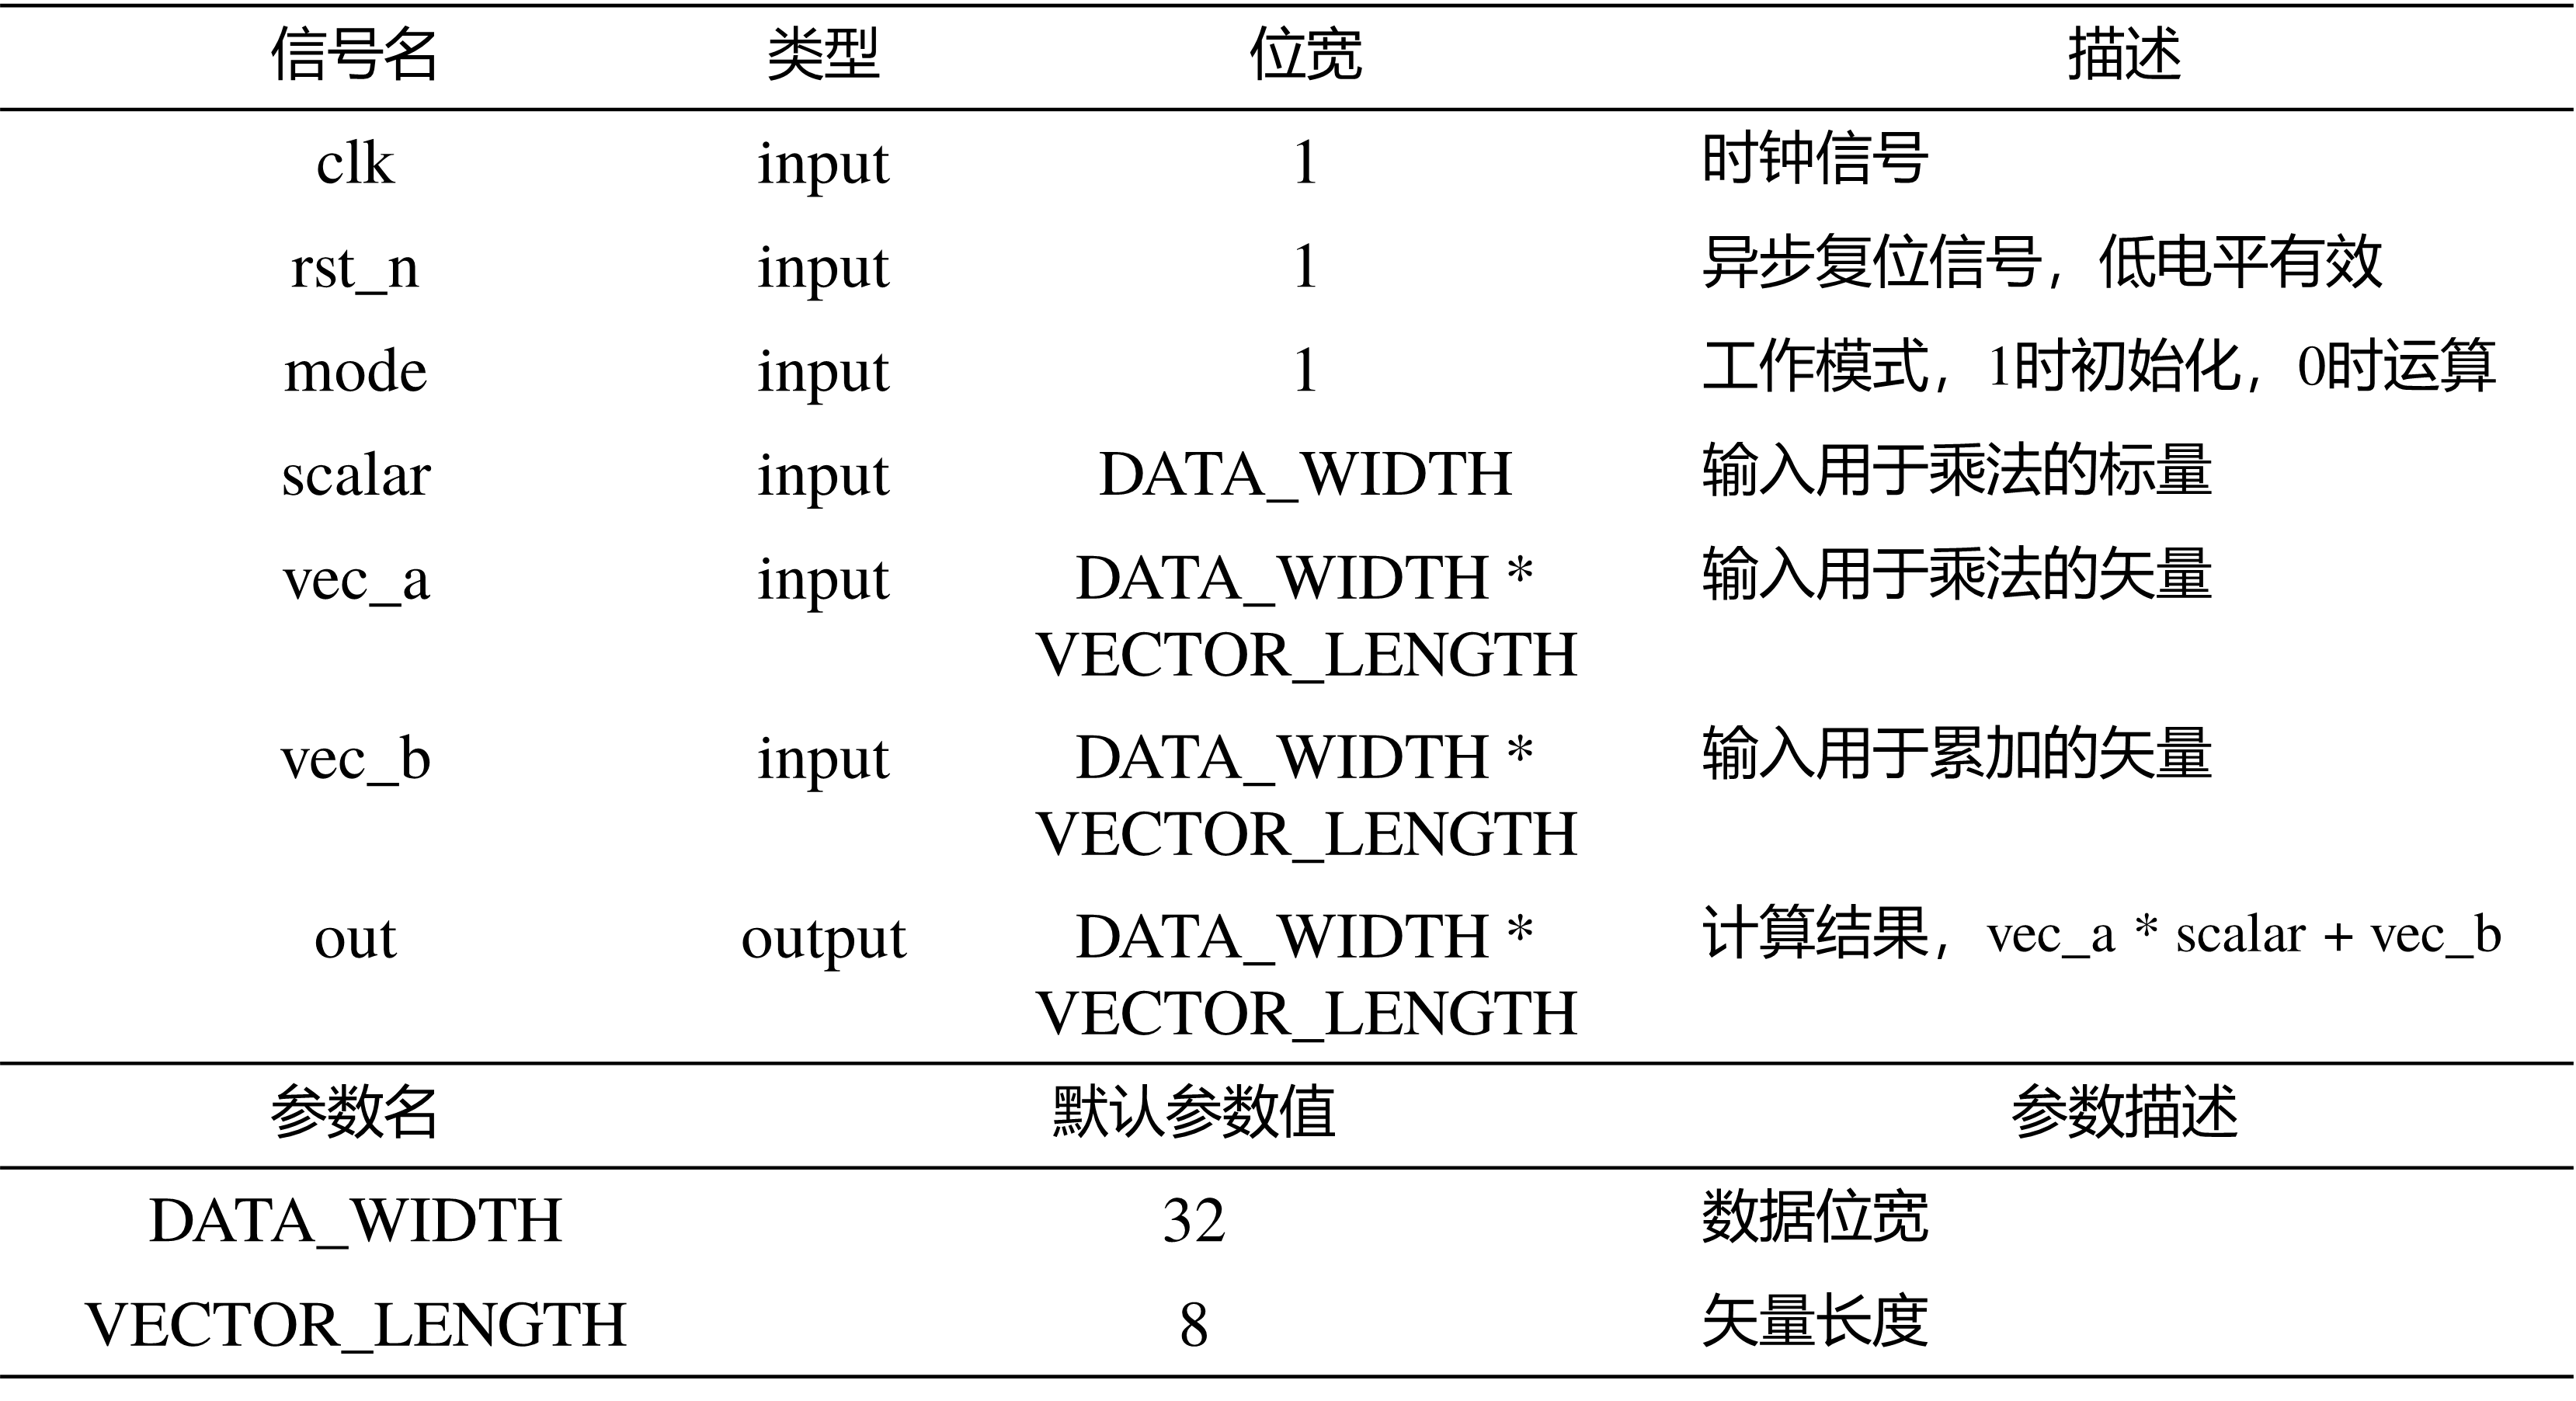
\includegraphics[width=16cm]{pic/MAC.png}
    \caption{标量矢量乘加单元端口说明}
\end{figure}

\subsection{控制单元}

控制单元根据当前指令以及之前的指令,产生相应的控制信号。控制寄存器和存储器的读写,以及各种数据选择器的选择信号。端口和参数说明如图14所示。

\begin{figure}[htbp]
    \centering
    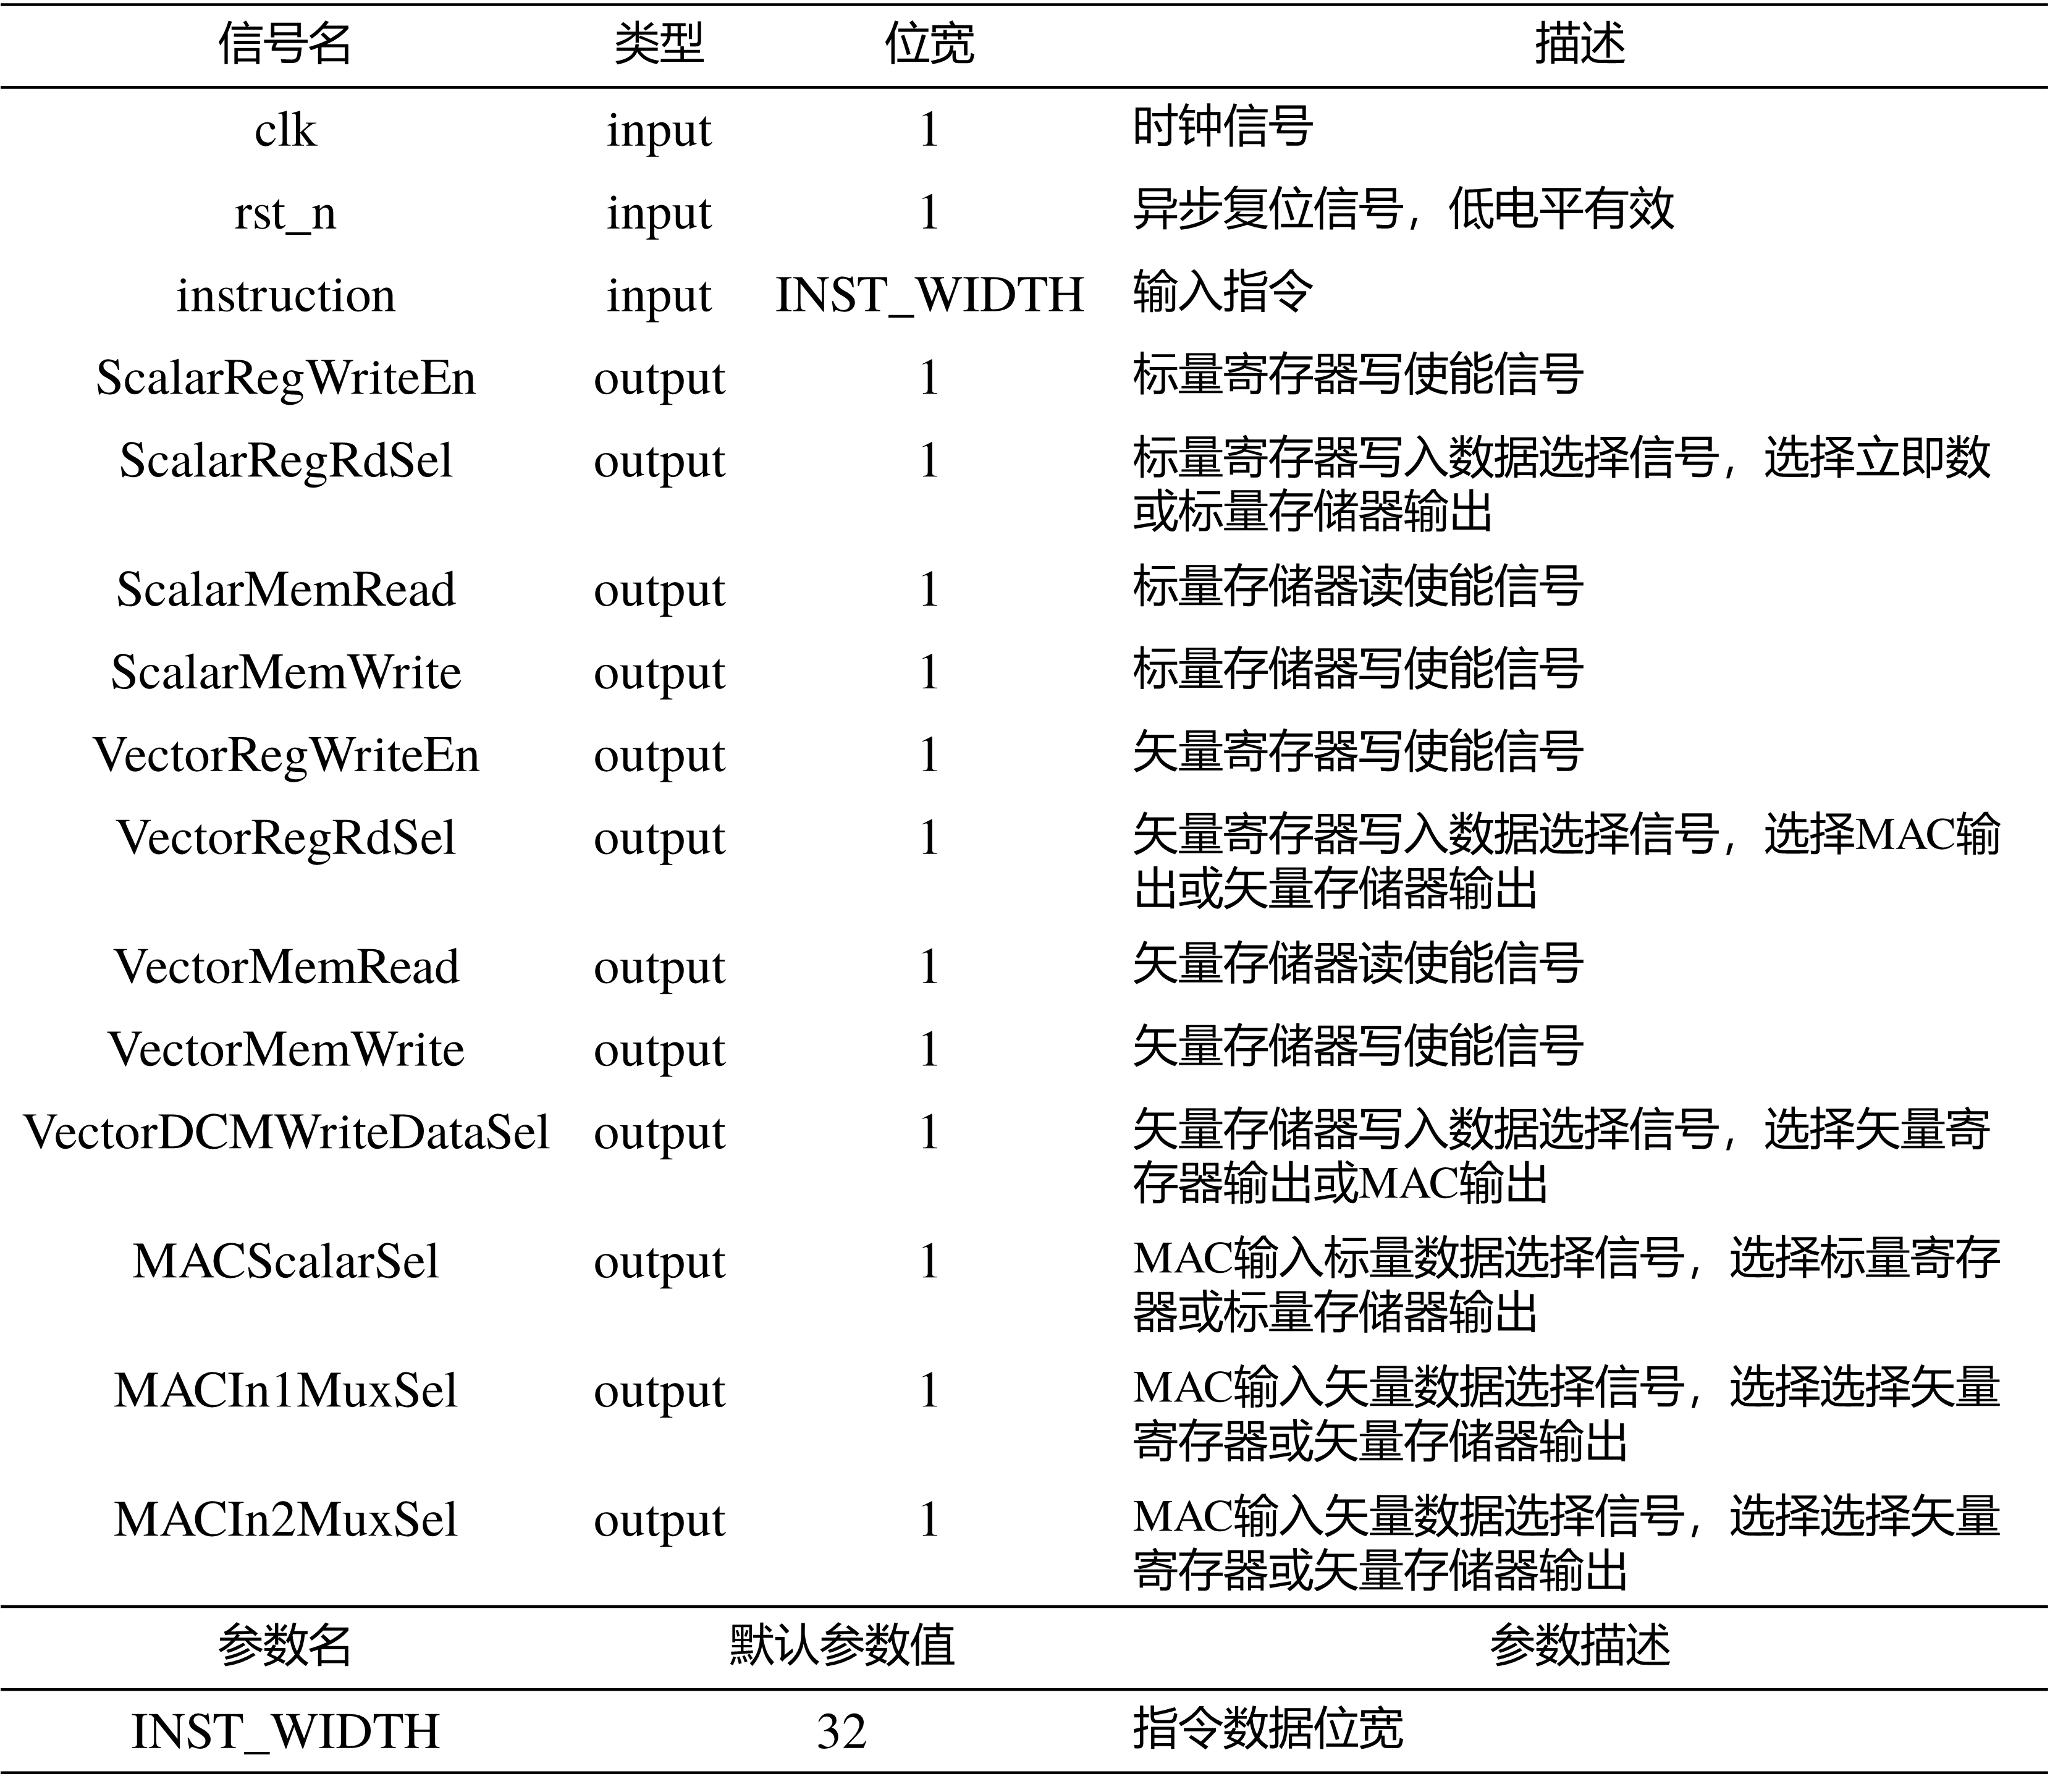
\includegraphics[width=16cm]{pic/Control.png}
    \caption{控制单元端口说明}
\end{figure}

\section{测试结果}
测试时,首先通过testbench在写入模式下对VPU的指令存储器、标量存储器和矢量存储器进行初始化,然后切换到执行模式运行指令。
最后在读取模式下从标量存储器和矢量存储器中读出结果进行验证。

\subsection{指令测试}

\subsubsection{MOV指令测试}
测试指令为 \verb|MOV R1 0xf| , \verb|MOV R2 0x3| 。结果应该是标量寄存器R1和R2被写入立即数0xf和0x3。

测试波形如图15所示。可以看到在译码器收到指令的同一个周期,立即数和写地址已经产生,此处的立即数是译码器直接产生的\verb|InstImm| ,而不是立即数生成模块的输出\verb|imm|。
同时标量寄存器的写入数据选择器切换到立即数通路,寄存器写使能信号有效,下一个周期立即数写入到寄存器中。

\begin{figure}[htbp]
    \centering
    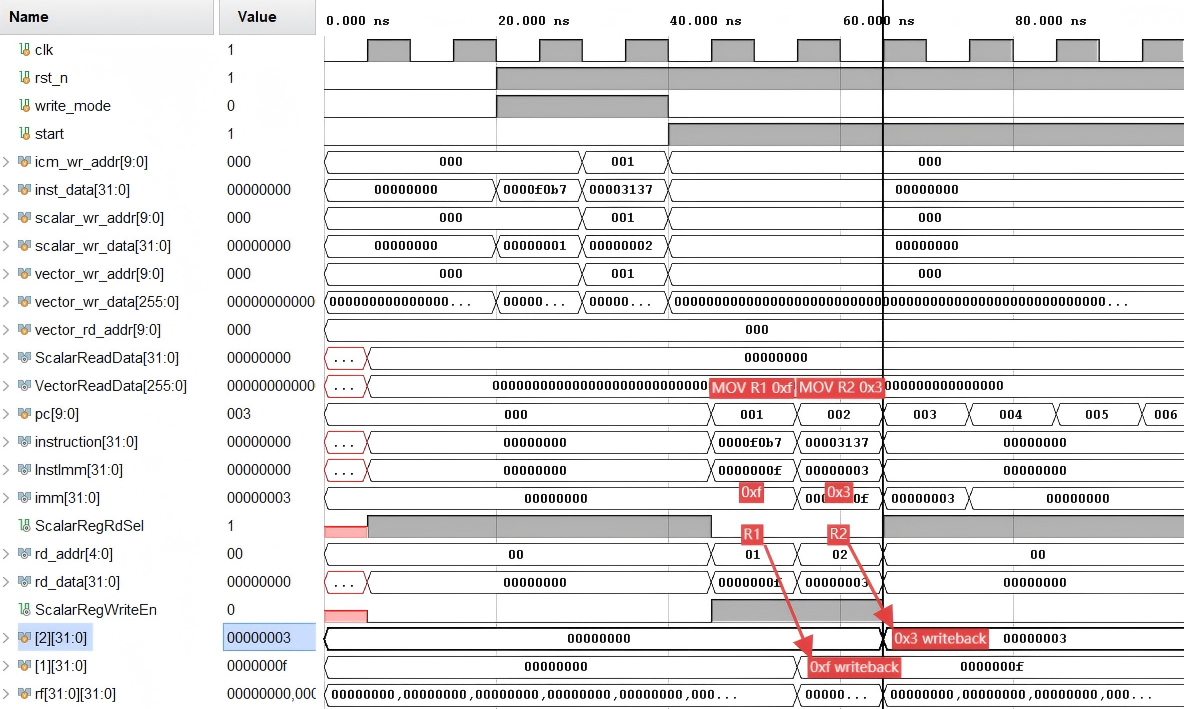
\includegraphics[width=16cm]{pic/VPU_MOV(1).png}
    \caption{MOV指令测试波形图}
\end{figure}

\subsubsection{LOAD指令测试}

测试LOAD指令需要有已经加载到存储器中的数据,因此需要先执行MOV指令将立即数加载到寄存器中。
测试指令为 \verb|MOV R1 0x1| , \verb|LOAD R2 R1 0x1| 。结果是标量寄存器R2被写入标量存储器的2号地址,实际第三个位置的数据(3)。

测试波形如图16所示。在译码器接收到指令的同一个周期完成译码,生成寄存器读地址。

下一个周期寄存器数据(rs1\_data)和立即数(imm)输出,相加后得到访存地址\\(ScalarMemAddr)。

下一个周期存储器数据(ScalarReadData)输出,同时寄存器写使能信号(ScalarRegWriteEn)有效,寄存器写地址(rd\_addr)也产生,寄存器写数据选择器(ScalarRegRdSel)切换到存储器数据通路。

下一个周期数据被写入到寄存器中。

\begin{figure}[htbp]
    \centering
    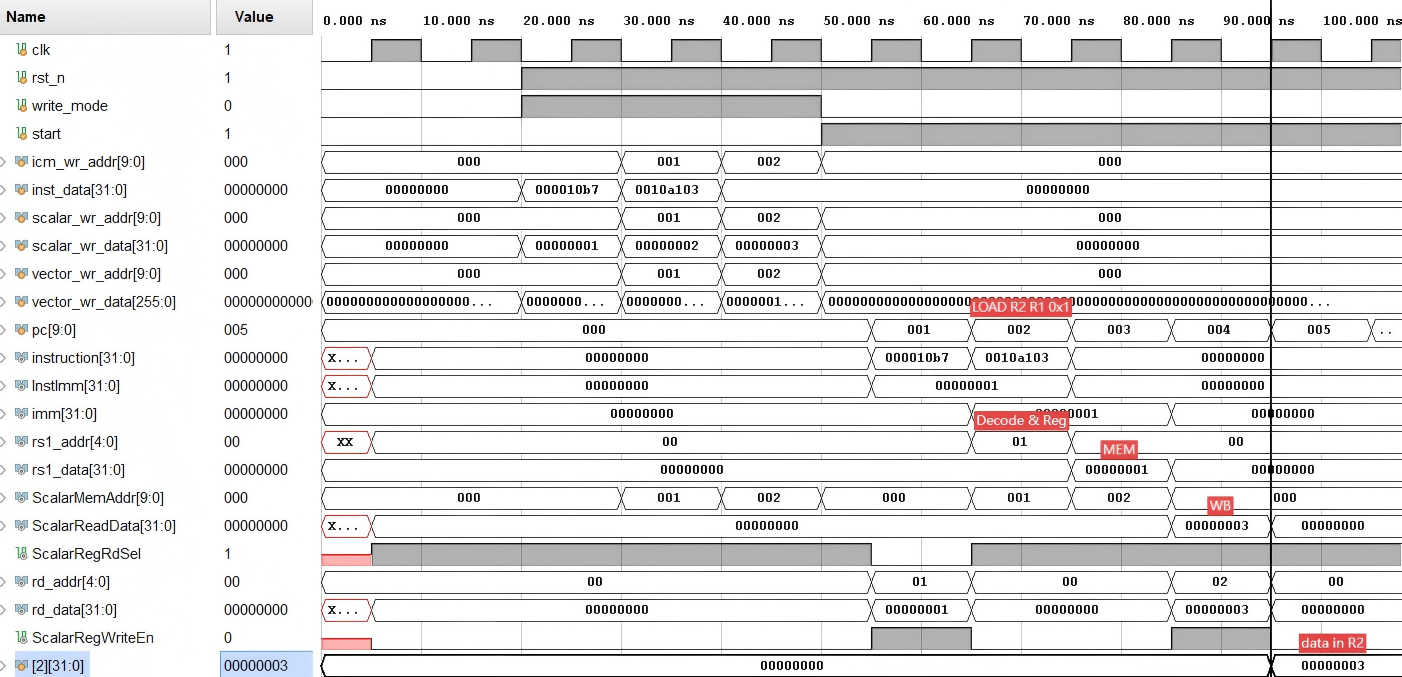
\includegraphics[width=16cm]{pic/VPU_LOAD(1).png}
    \caption{LOAD指令测试波形图}
\end{figure}

\subsubsection{VLOAD指令测试}

测试指令为 \verb|MOV R1 0x1| , \verb|VLOAD VR3 R1 0x1| 。结果是矢量寄存器VR3被写入矢量存储器2号地址,实际第三个位置的数据\verb|[0x11, 0x12, 0x13, 0x14, 0x15, 0x16, 0x17, 0x18]| 。

测试波形图如图17所示。在译码器接收到指令的同一个周期完成译码,生成寄存器读地址。

下一个周期寄存器数据(rs1\_data)和立即数(imm)输出,相加后得到访存地址(VectorMemAddr)。

下一个周期存储器数据(VectorReadData)输出,同时寄存器写使能信号(VectorRegWriteEn)有效,寄存器写地址(vrd\_addr)也产生,寄存器写数据选择器(VectorRegRdSel)切换到存储器数据通路。

下一个周期数据被写入到寄存器中。

\begin{figure}[htbp]
    \centering
    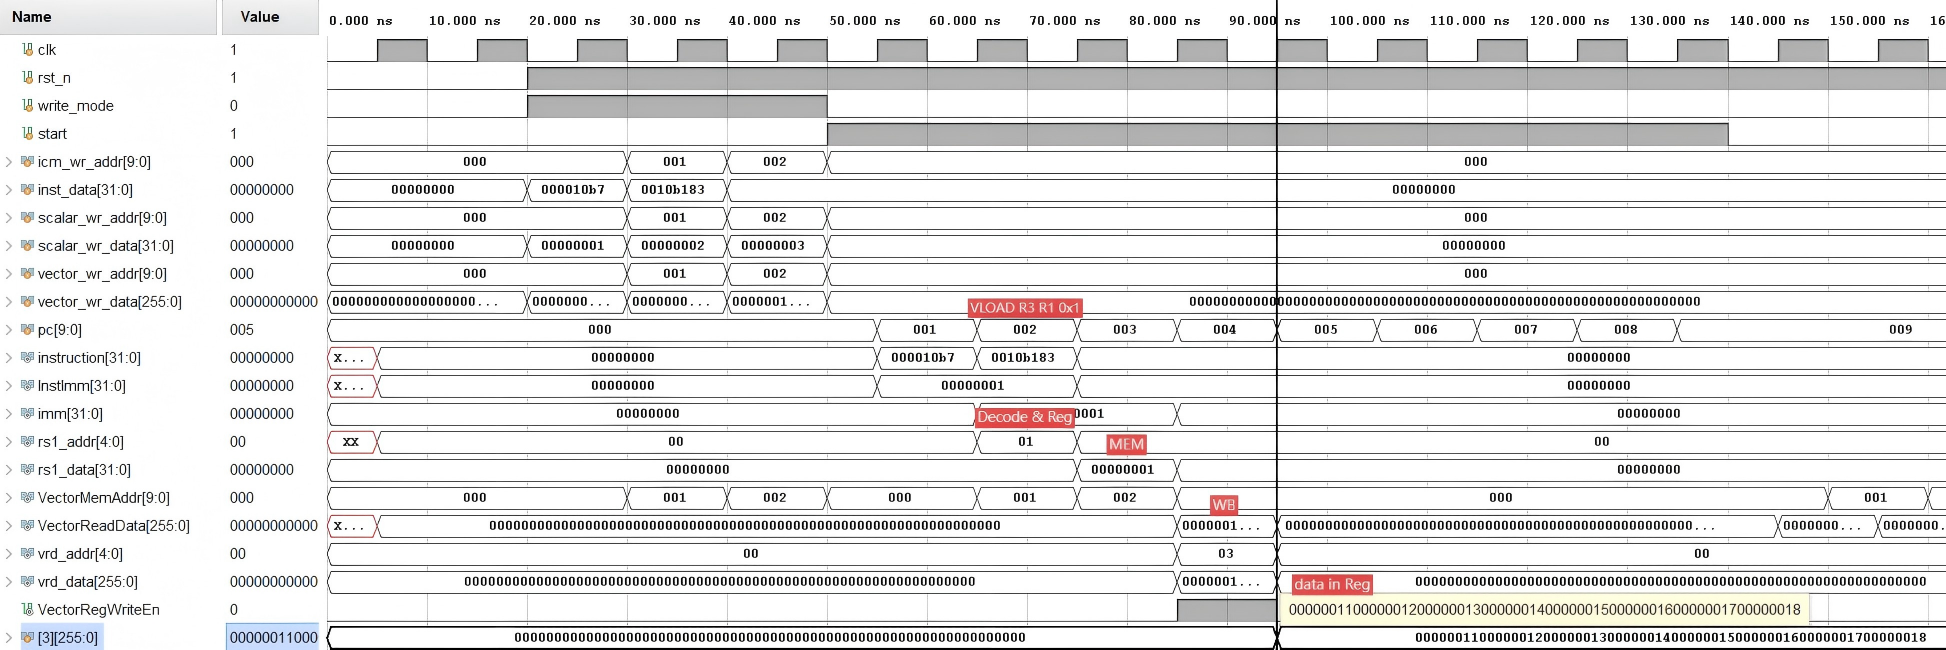
\includegraphics[width=16cm]{pic/VPU_VLOAD(1).png}
    \caption{VLOAD指令测试波形图}
\end{figure}

\subsubsection{MAC指令测试}

MAC的测试分为两种情况,一种是reset工作模式,一种是MAC工作模式,测试时按照先reset再MAC的顺序编写指令,每次执行MAC指令前都要用LOAD和VLOAD加载操作数。

reset模式测试指令为 \verb|MOV R1 0x1| , \verb|LOAD R3 R1 0x1| ,\verb|VLOAD VR3 R1 0x2| , \verb|MAC VR4 VR3 R3 1|

MAC模式测试指令为   \verb|LOAD R2 R1 0x1| ,\verb|VLOAD VR2 R1 0x2| , \verb|MAC VR4 VR2 R2 0|

第一个的结果应该是VR4被写入了VR3的值,第二个的结果应该是VR4被写入了(VR2*R2+VR4)的值,在测试中是\verb|[0x13, 0x16, 0x19, 0x1c, 0x1f, 0x22, 0x25, 0x28]|

测试波形图如图18(a)(b)所示。

可以看到两种指令的执行时序是一样的,发出指令的下一个周期MAC模块的输入数据到位,下一个周期计算结果输出,下一个周期写回到寄存器。
注意到由于LOAD和VLOAD指令发出较晚,需要数据前馈,在MAC指令发出的后一个周期数据直接从两个存储器前馈到MAC模块的输入端,
这是通过改变输入端选择器(MACIn1MUXSel和MACIn2MUXSel)的数据通路实现的。

\begin{figure}[htbp]
    \centering
    \subfigure[reset模式测试波形]{
        \label{Fig.sub.1}
        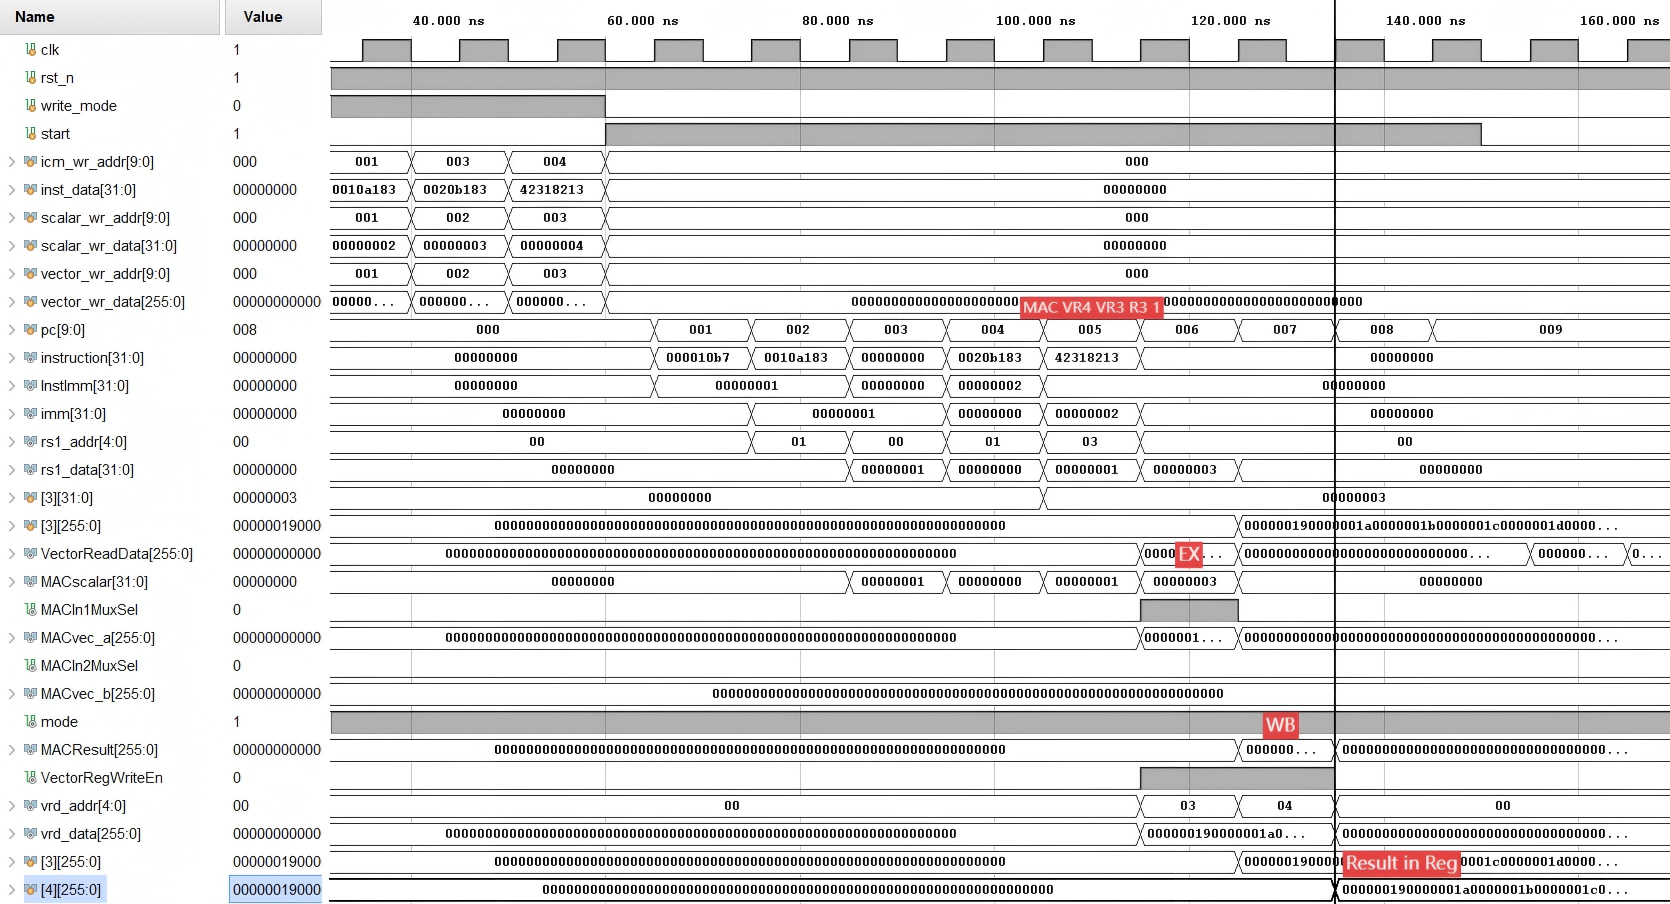
\includegraphics[width=14cm]{pic/VPU_MAC1(1).png}}
    \subfigure[MAC模式测试波形]{
        \label{Fig.sub.2}
        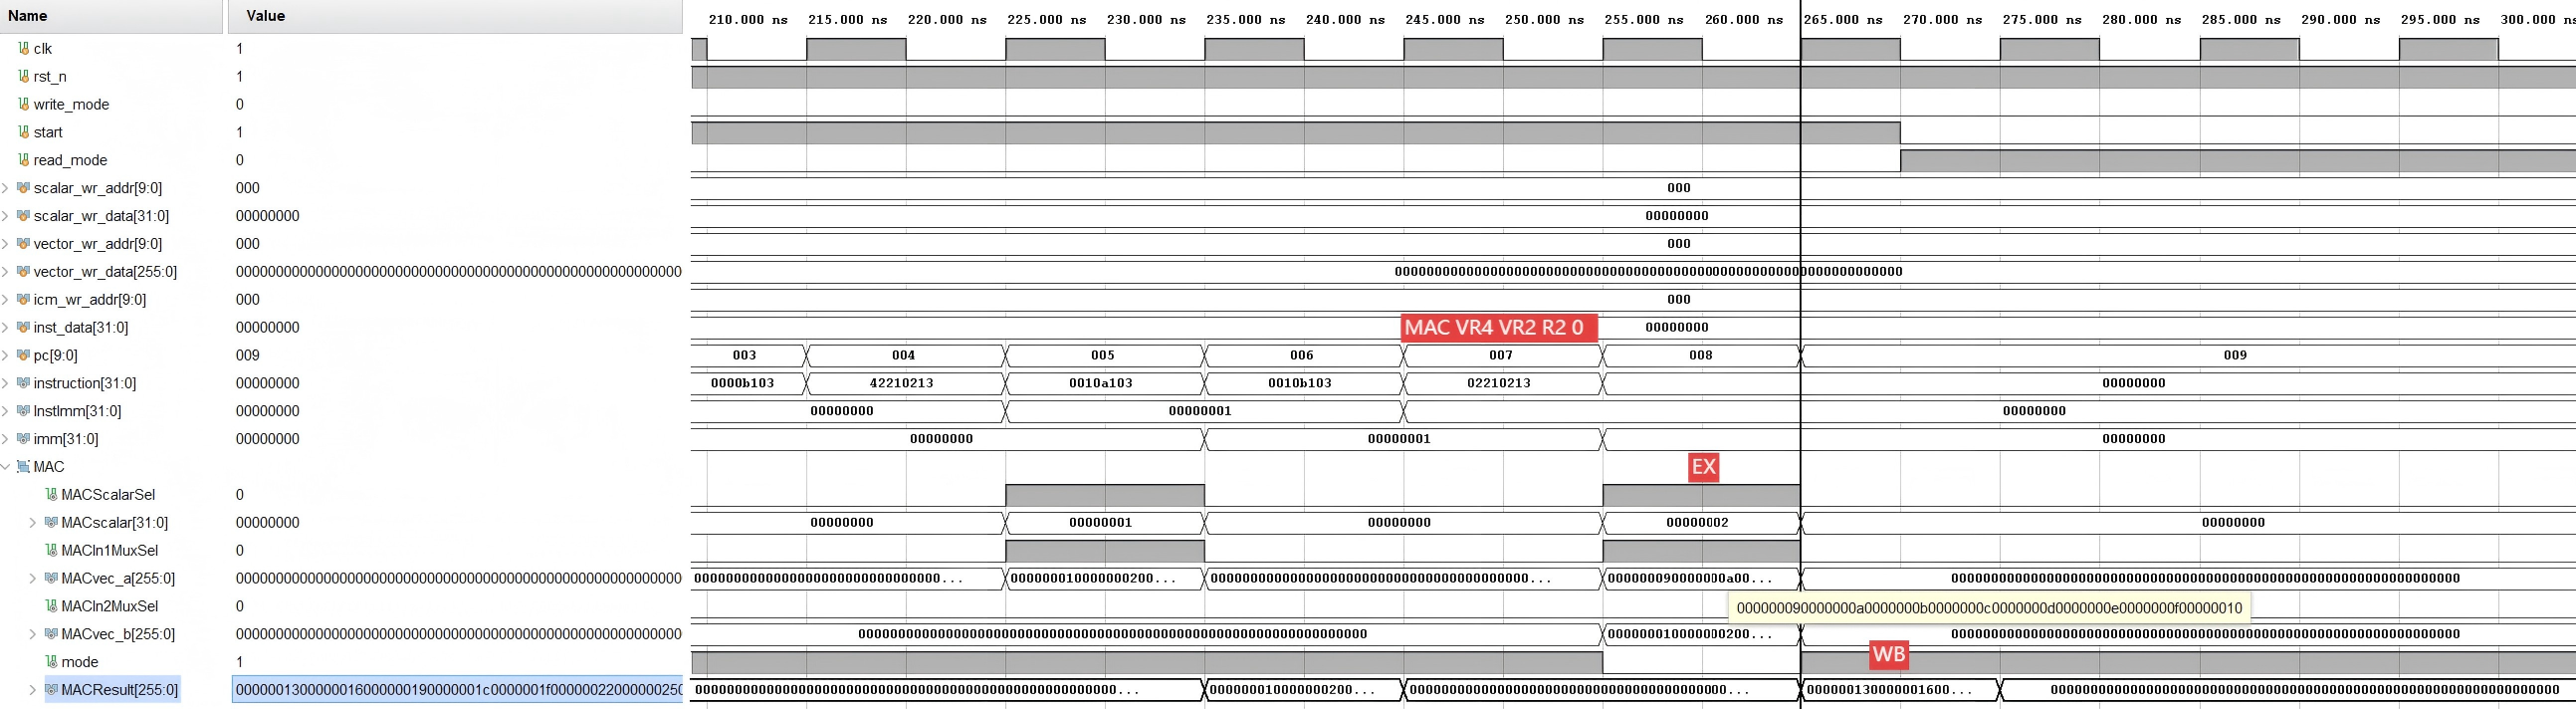
\includegraphics[width=12.7cm]{pic/VPU_MAC0(1).png}}
    \caption{MAC指令测试波形图}
    \label{Fig.main}
\end{figure}

\subsubsection{VSTORE指令测试}

VSTORE阶段需要存储MAC计算完成的结果,测试指令为\verb|MOV R1 0x3|, \verb|VSTORE VR4 R1 0x0| 。结果应该是矢量存储器的3号地址,
实际第四个位置被写入VR4中的数据\\\verb|[0x13, 0x16, 0x19, 0x1c, 0x1f, 0x22, 0x25, 0x28]| 。

测试波形如图19所示。

\begin{figure}[htbp]
    \centering
    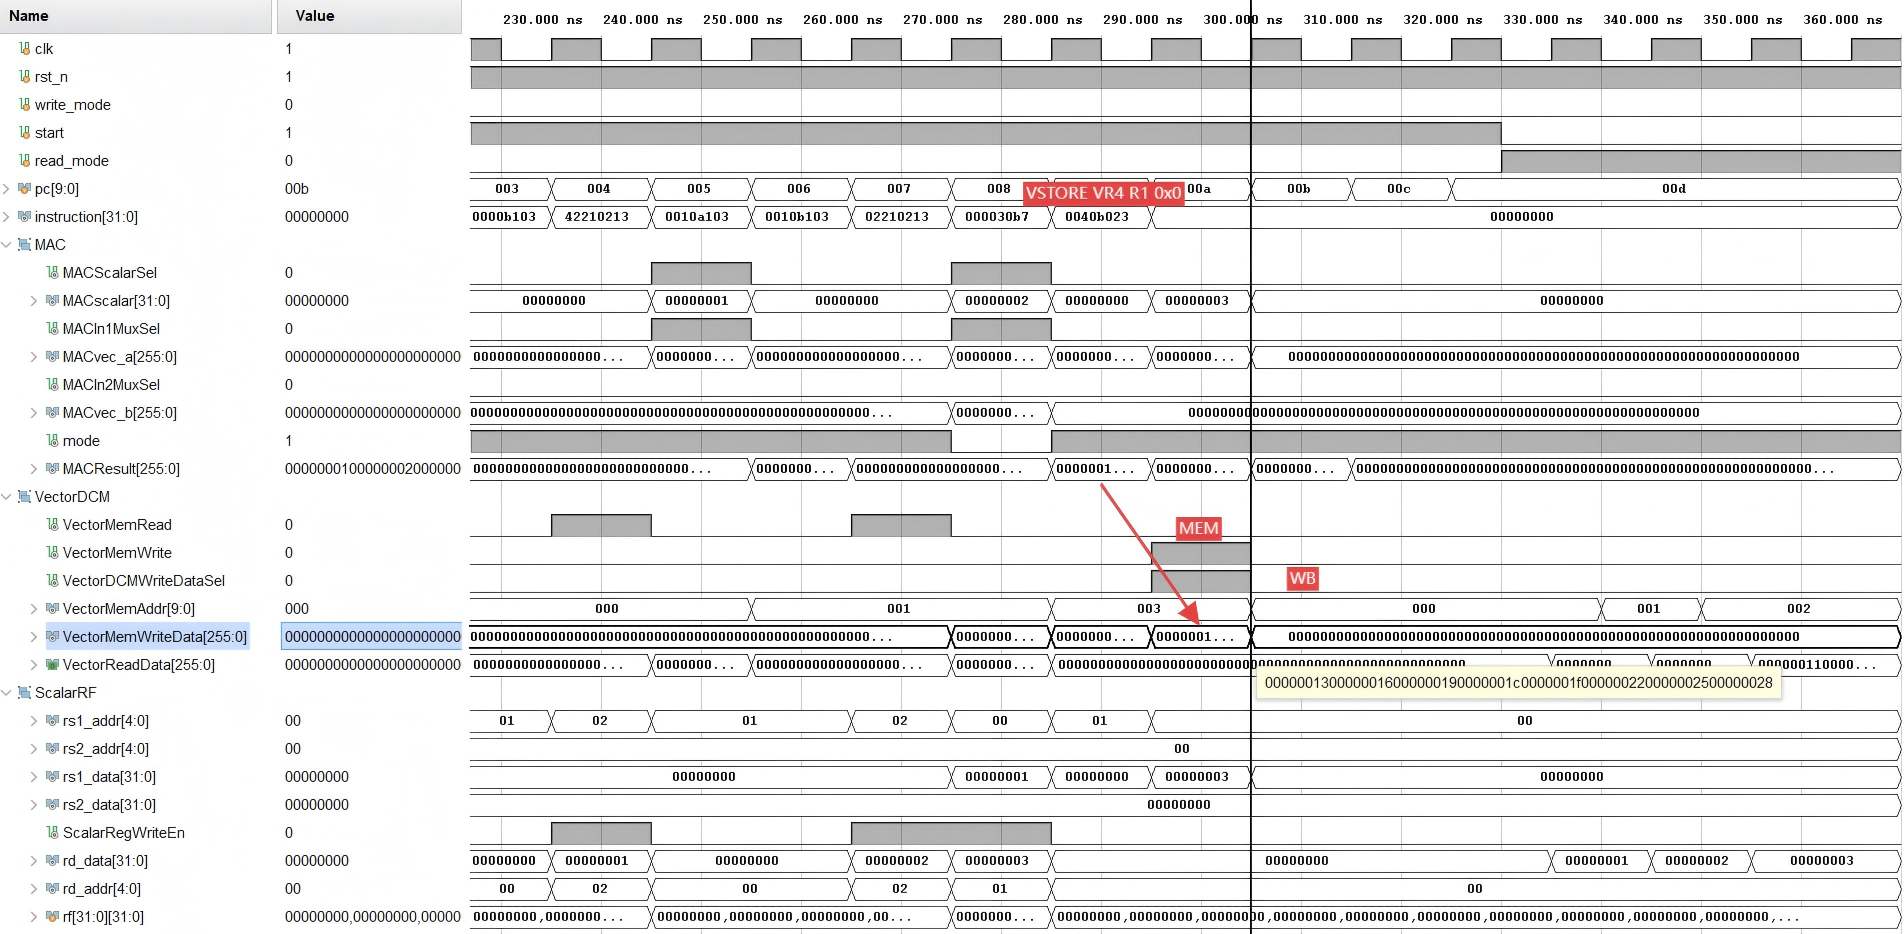
\includegraphics[width=16cm]{pic/VPU_VSTORE(1).png}
    \caption{VSTORE指令测试波形图}
\end{figure}

在接收到指令的下一个周期,矢量存储器的写使能信号(VectorMemWrite)有效,写地址(VectorMemAddr)产生,写数据(VectorMemWriteData)直接从MAC单元前馈到存储器的输入。
下一个周期数据写入存储器,此时矢量存储器写入数据选择器(VectorDCMWriteDataSel)选择MAC的数据通路。

\subsubsection{STORE指令测试}

STORE指令的测试指令为 \verb|MOV R1, 0xf|,\verb|MOV R2, 0x2| ,\verb|STORE R1, R2, 0x1| 。
结果应该是取R1的数据(0xf),写入R2的值(0x2)加上0x1得到的地址(0x3),即在标量存储器的0x3号地址处写入0xf。

测试波形如图20所示。

\begin{figure}[htbp]
    \centering
    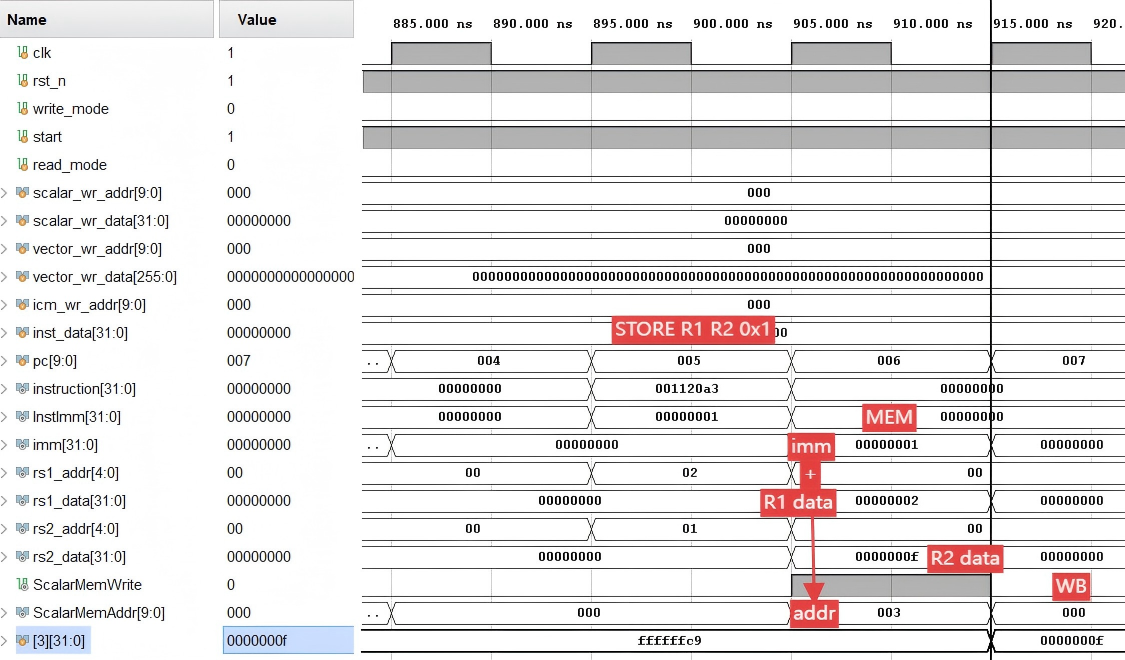
\includegraphics[width=16cm]{pic/VPU_STORE(1).png}
    \caption{STORE指令测试波形图}
\end{figure}

在接收到指令的写一个周期,标量存储器的使能信号有效,同时立即数和R1数据相加得到访存地址,R2数据作为写入数据,下一个周期写入标量存储器中。

\subsection{整体测试}
\subsubsection{测试数据}
测试输入为三个8*8的矩阵,一个存储在向量缓存中,两个存储在标量缓存中,计算矩阵的乘加运算,测试数据为随机生成,如下:
\begin{equation}
Matrix_1
=
\left[
\begin{array}{cccccccc}
    -69 & 95  & 73  & -55 & 17  & 32  & -16 & 24  \\
    100 & -93 & 56  & 41  & 47  & 83  & -69 & 4   \\
    77  & -83 & -26 & -78 & -14 & -27 & 75  & 1   \\
    -54 & 62  & 88  & 13  & -18 & 39  & 0   & 97  \\
    -12 & 85  & 58  & -80 & 44  & 53  & -99 & 66  \\
    -37 & 7   & 99  & 25  & -61 & 18  & 55  & -92 \\
    -70 & 49  & -34 & 81  & 60  & -47 & 28  & -85 \\
    -2  & 100 & -59 & 36  & -77 & 72  & 11  & -63 
\end{array}
\right]
\end{equation}

\begin{equation}
Matrix_2
=
\left[
\begin{array}{cccccccc}
    -88 & 14  & 67  & -99 & 53  & 80  & -41 & 22  \\
    -7  & 91  & -62 & 38  & 100 & -56 & 19  & -84 \\
    -35 & 60  & 27  & -90 & 45  & 8   & -30 & 73  \\
    59  & -13 & 92  & -75 & 31  & -68 & 85  & -24 \\
    -96 & 70  & 2   & 99  & -50 & 63  & -17 & 44  \\
    81  & -28 & 54  & -61 & 12  & 97  & -79 & 6   \\
    -58 & 35  & 100 & -87 & 29  & -32 & 76  & -9  \\
    40  & -95 & 21  & 65  & -73 & 58  & -12 & 90
\end{array}
\right]
\end{equation}

\begin{equation}
Matrix_3
=
\left[
\begin{array}{cccccccc}
    81 & -44 & 56 & -90 &  13 & 67 & -38 &  72\\
   -99 &  35 &-73 &  40 &  86 &-65 &  17 &  33\\
    27 & -88 & 62 & -41 &  19 & 77 & -56 &  84\\
   -13 &  95 &-22 &  59 & -80 & 36 &  48 & -71\\
    61 & -24 & 79 & -92 &  55 & 12 & -38 &  70\\
   -47 &  81 &-66 &  28 & -35 & 99 & -21 &  10\\
    53 & -60 & 44 & -85 &  72 &-18 &  25 & -97\\
   -31 &  67 &-49 &  90 & -76 & 38 &  63 & -29
\end{array}
\right]
\end{equation}

理论结果为

\begin{equation}
\left[
\begin{array}{cccccccc}
    2536  &  10184 & -12880 &  10589 &  4754  & -370   & -6590  &  467   \\
   -1416  & -6030  &  15437 & -15656 & -3770  &  24255 & -16693 &  16696 \\
   -15013 & -4803  &  8524  & -8827  & -5310  &  10138 & -2581  &  7361  \\
    10759 & -1475  &  195   &  1010  &  1908  &  339   & -2034  &  7817  \\
    2223  &  3924  & -17353 &  19132 & -1204  &  15105 & -19722 &  7905  \\
    1614  &  11706 &  6412  & -24730 &  15511 & -13354 &  5683  & -6116  \\
   -2752  &  14897 & -2553  &  6538  &  5696  & -20747 &  17572 & -15723 \\
    13700 &  4095  & -1153  & -10369 &  17911 & -10515 &  4088  & -22369
\end{array}
\right]
\end{equation}

\subsubsection{测试步骤}
首先,将三个矩阵和指令输入存储器,矩阵1输入到标量存储器中,矩阵2,3输入到矢量存储器中,指令存储到指令存储器中。
三个矩阵都默认连续存储,矩阵1占用标量存储器0x0-0x3f的地址空间,矩阵2占用矢量存储器0x0-0x7的地址空间,矩阵3占用矢量存储器0x8-0x10的地址空间。
三个矩阵通过VPU模块的写模式写入存储器,在testbench中实现。图22是写入过程的波形图。

\begin{figure}[htbp]
    \centering
    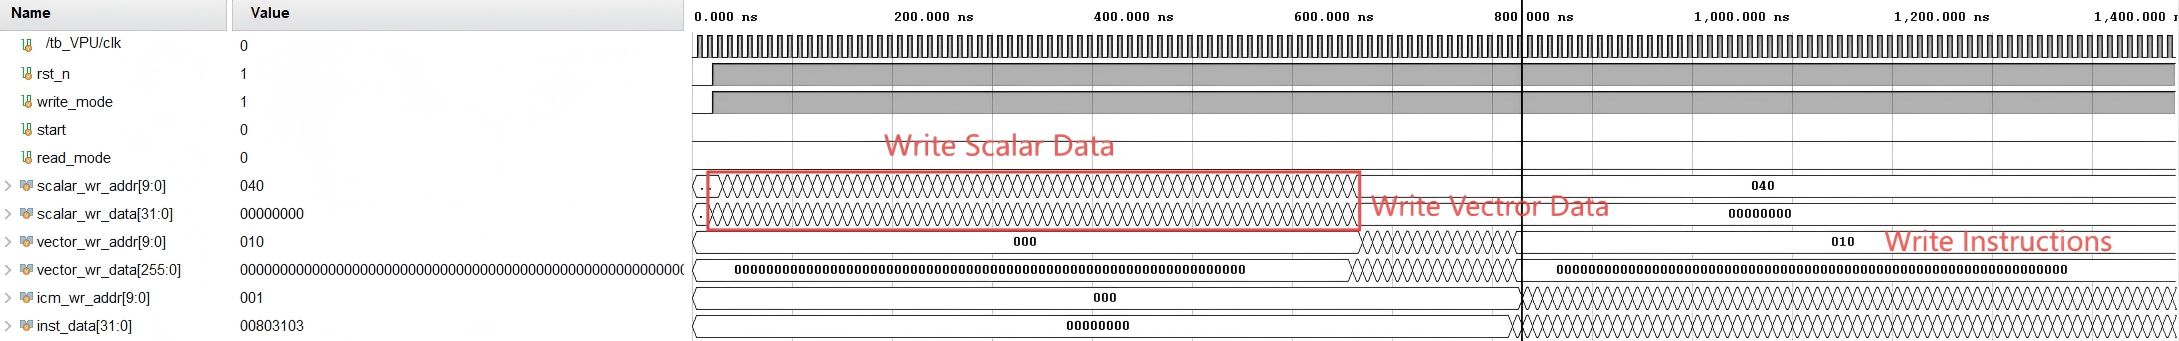
\includegraphics[width=16cm]{pic/write_wfm(1).png}
    \caption{写入模式波形图}
\end{figure}

测试用的汇编代码由脚本\verb|gen_inst.py|生成,部分代码如下,完整代码详见\verb|vpu_test.asm| 。
\lstset{
 columns=fixed,       
 numbers=left,                                        % 在左侧显示行号
 numberstyle=\tiny\color{gray},                       % 设定行号格式
 frame=none,                                          % 不显示背景边框
 backgroundcolor=\color[RGB]{245,245,244},            % 设定背景颜色
 keywordstyle=\color[RGB]{40,40,255},                 % 设定关键字颜色
 numberstyle=\footnotesize\color{darkgray},           
 commentstyle=\it\color[RGB]{0,96,96},                % 设置代码注释的格式
 stringstyle=\rmfamily\slshape\color[RGB]{128,0,0},   % 设置字符串格式
 showstringspaces=false,                              % 不显示字符串中的空格
 language=c++,                                        % 设置语言
}
\begin{lstlisting}
    // line1
    MOV     R1,       0x0     // R1 = 0x0
    VLOAD  VR2,  R0,  0x8     // VR2 = Matrix_3[0][:]
    VMAC   VR3,  R2,  VR2, 1  // VR3 = VR2

    LOAD    R2,  R1,  0x0     // R2 = Matrix_1[0][0]
    VLOAD  VR2,  R0,  0x0     // VR2 = Matrix_2[0][:]
    VMAC   VR3,  R2,  VR2, 0  // VR3 = R2 * VR2 + VR3

    LOAD    R2,  R1,  0x1     // R2 = Matrix_1[0][1]
    VLOAD  VR2,  R0,  0x1     // VR2 = Matrix_2[1][:]
    VMAC   VR3,  R2,  VR2, 0  // VR3 = R2 * VR2 + VR3

    LOAD    R2,  R1,  0x2     // R2 = Matrix_1[0][2]
    VLOAD  VR2,  R0,  0x2     // VR2 = Matrix_2[2][:]
    VMAC   VR3,  R2,  VR2, 0  // VR3 = R2 * VR2 + VR3

    LOAD    R2,  R1,  0x3     // R2 = Matrix_1[0][3]
    VLOAD  VR2,  R0,  0x3     // VR2 = Matrix_2[3][:]
    VMAC   VR3,  R2,  VR2, 0  // VR3 = R2 * VR2 + VR3

    LOAD    R2,  R1,  0x4     // R2 = Matrix_1[0][4]
    VLOAD  VR2,  R0,  0x4     // VR2 = Matrix_2[4][:]
    VMAC   VR3,  R2,  VR2, 0  // VR3 = R2 * VR2 + VR3

    LOAD    R2,  R1,  0x5     // R2 = Matrix_1[0][5]
    VLOAD  VR2,  R0,  0x5     // VR2 = Matrix_2[5][:]
    VMAC   VR3,  R2,  VR2, 0  // VR3 = R2 * VR2 + VR3

    LOAD    R2,  R1,  0x6     // R2 = Matrix_1[0][6]
    VLOAD  VR2,  R0,  0x6     // VR2 = Matrix_2[6][:]
    VMAC   VR3,  R2,  VR2, 0  // VR3 = R2 * VR2 + VR3

    LOAD    R2,  R1,  0x7     // R2 = Matrix_1[0][7]
    VLOAD  VR2,  R0,  0x7     // VR2 = Matrix_2[7][:]
    VMAC   VR3,  R2,  VR2, 0  // VR3 = R2 * VR2 + VR3

    MOV     R3,       0x10    // R3 = 0x10(after matrix3)
    VSTORE  R3,  VR2          // store VR2 to VectorDCM[16]

    ...

    // line8
    MOV     R1,       0x38     // R1 = 0x38
    VLOAD  VR2,  R0,  0xf     // VR2 = Matrix_3[7][:]
    VMAC   VR3,  R2,  VR2, 1  // VR3 = VR2

    LOAD    R2,  R1,  0x0     // R2 = Matrix_1[7][0]
    VLOAD  VR2,  R0,  0x0     // VR2 = Matrix_2[0][:]
    VMAC   VR3,  R2,  VR2, 0  // VR3 = R2 * VR2 + VR3

    LOAD    R2,  R1,  0x1     // R2 = Matrix_1[7][1]
    VLOAD  VR2,  R0,  0x1     // VR2 = Matrix_2[1][:]
    VMAC   VR3,  R2,  VR2, 0  // VR3 = R2 * VR2 + VR3

    LOAD    R2,  R1,  0x2     // R2 = Matrix_1[7][2]
    VLOAD  VR2,  R0,  0x2     // VR2 = Matrix_2[2][:]
    VMAC   VR3,  R2,  VR2, 0  // VR3 = R2 * VR2 + VR3

    LOAD    R2,  R1,  0x3     // R2 = Matrix_1[7][3]
    VLOAD  VR2,  R0,  0x3     // VR2 = Matrix_2[3][:]
    VMAC   VR3,  R2,  VR2, 0  // VR3 = R2 * VR2 + VR3

    LOAD    R2,  R1,  0x4     // R2 = Matrix_1[7][4]
    VLOAD  VR2,  R0,  0x4     // VR2 = Matrix_2[4][:]
    VMAC   VR3,  R2,  VR2, 0  // VR3 = R2 * VR2 + VR3

    LOAD    R2,  R1,  0x5     // R2 = Matrix_1[7][5]
    VLOAD  VR2,  R0,  0x5     // VR2 = Matrix_2[5][:]
    VMAC   VR3,  R2,  VR2, 0  // VR3 = R2 * VR2 + VR3

    LOAD    R2,  R1,  0x6     // R2 = Matrix_1[7][6]
    VLOAD  VR2,  R0,  0x6     // VR2 = Matrix_2[6][:]
    VMAC   VR3,  R2,  VR2, 0  // VR3 = R2 * VR2 + VR3

    LOAD    R2,  R1,  0x7     // R2 = Matrix_1[7][7]
    VLOAD  VR2,  R0,  0x7     // VR2 = Matrix_2[7][:]
    VMAC   VR3,  R2,  VR2, 0  // VR3 = R2 * VR2 + VR3

    MOV     R3,       0x17    // R3 = 0x17(after matrix3)
    VSTORE  R3,  VR2          // store VR2 to VectorDCM[23]

\end{lstlisting}

再使用脚本\verb|gen_inst_code.py|将汇编代码转换成机器码,按照testbench的格式输出。

输入数据完成后,启动VPU,在执行完所有指令后进入读取模式。
依次从标量存储器和矢量存储器中读取计算结果。
读取的波形图如图22所示。

\begin{figure}[htbp]
    \centering
    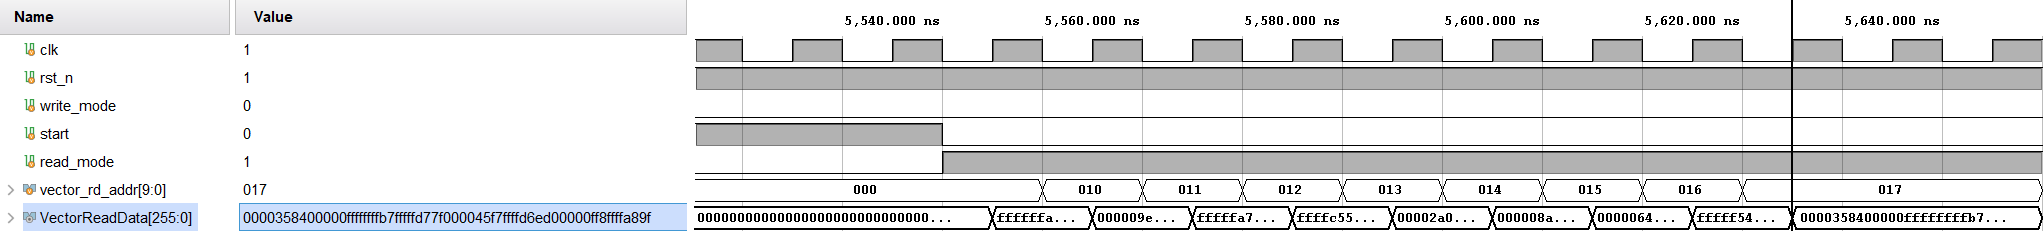
\includegraphics[width=16cm]{pic/read_wfm.png}
    \caption{读取模式波形图}
\end{figure}

将计算结果读出并在tcl窗口中打印,结果如图23所示。

\begin{figure}[htbp]
    \centering
    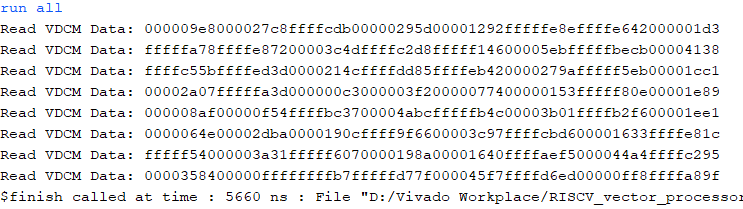
\includegraphics[width=16cm]{pic/matrix_result.png}
    \caption{计算结果}
\end{figure}

\lstset{
 columns=fixed,       
 numbers=left,                                        % 在左侧显示行号
 numberstyle=\tiny\color{gray},                       % 设定行号格式
 frame=none,                                          % 不显示背景边框
 backgroundcolor=\color[RGB]{245,245,244},            % 设定背景颜色
 keywordstyle=\color[RGB]{40,40,255},                 % 设定关键字颜色
 numberstyle=\footnotesize\color{darkgray},           
 commentstyle=\it\color[RGB]{0,96,96},                % 设置代码注释的格式
 stringstyle=\rmfamily\slshape\color[RGB]{128,0,0},   % 设置字符串格式
 showstringspaces=false,                              % 不显示字符串中的空格
 language=c++,                                        % 设置语言
}

对应的十进制数与理想结果相同,表明处理器可以正常工作。

\section{性能分析}

\subsection{延时分析}
时序报告如图24所示。
在100MHz时钟下,时钟周期为10ns,建立时间裕度2.146ns,保持时间裕度0.02ns。

\begin{figure}[htbp]
    \centering
    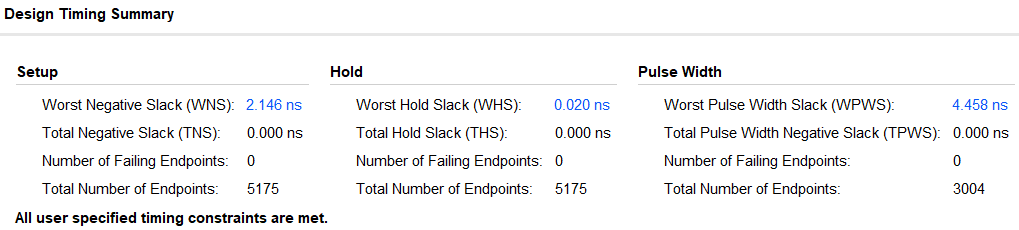
\includegraphics[width=16cm]{pic/timing.png}
    \caption{时序报告}
\end{figure}

\subsection{功耗分析}
功耗分析报告如图25所示。

\begin{figure}[htbp]
    \centering
    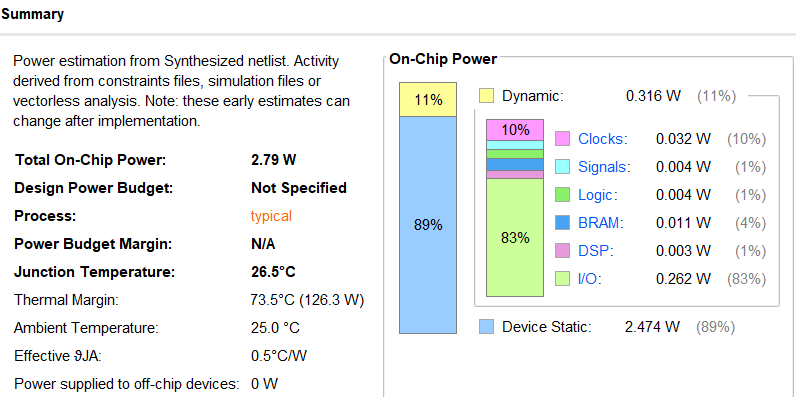
\includegraphics[width=16cm]{pic/power.png}
    \caption{功耗报告}
\end{figure}

\subsection{资源占用}

资源占用报告如图26所示。共使用了6640个查找表,10134个寄存器,9.5个BRAM,24个DSP

\begin{figure}[htbp]
    \centering
    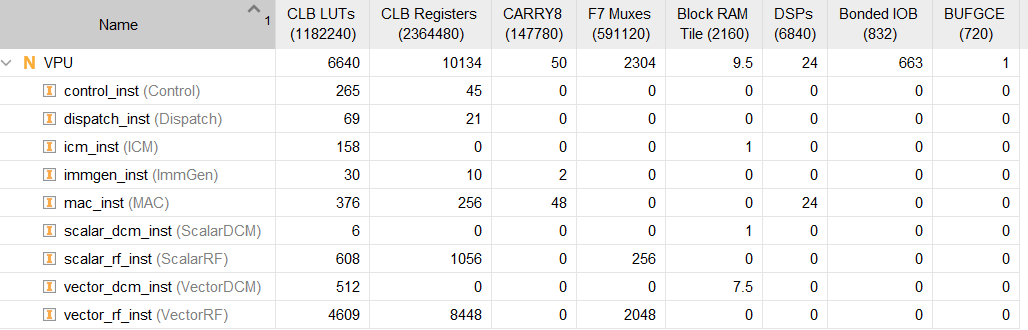
\includegraphics[width=16cm]{pic/utilization.png}
    \caption{资源占用报告}
\end{figure}

\section{优化分析}

在优化方面,主要对汇编代码进行优化。从原先每次计算都要读取两个数据变为每次仅读取一个标量数据,减少了指令数量和访存次数。
具体计算过程如图27所示。

\begin{figure}[htbp]
    \centering
    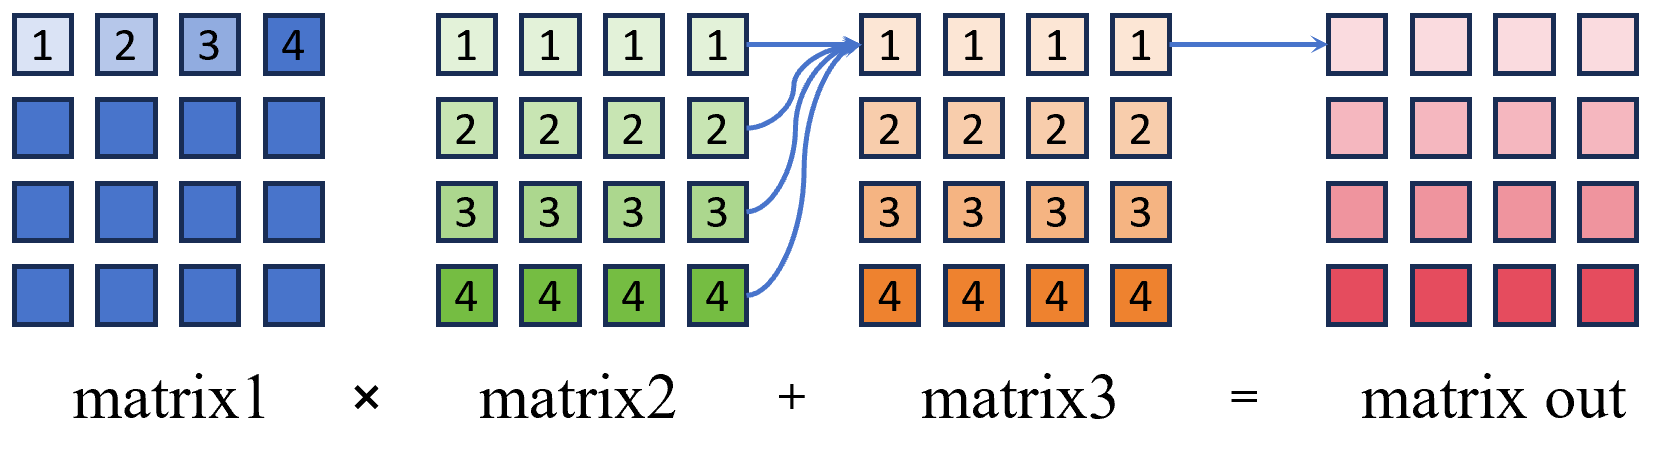
\includegraphics[width=14cm]{pic/calcu_ill.png}
    \caption{计算顺序示意图}
\end{figure}

图中是4*4的矩阵乘加运算,编号相同的标量和矢量乘加后加到结果的第一行,图中仅画出了第一行的计算过程,其余同理。这样就将矩阵乘法拆分成了标量矢量乘法。

实际指令级的计算过程如图28所示。

\begin{figure}[htbp]
    \centering
    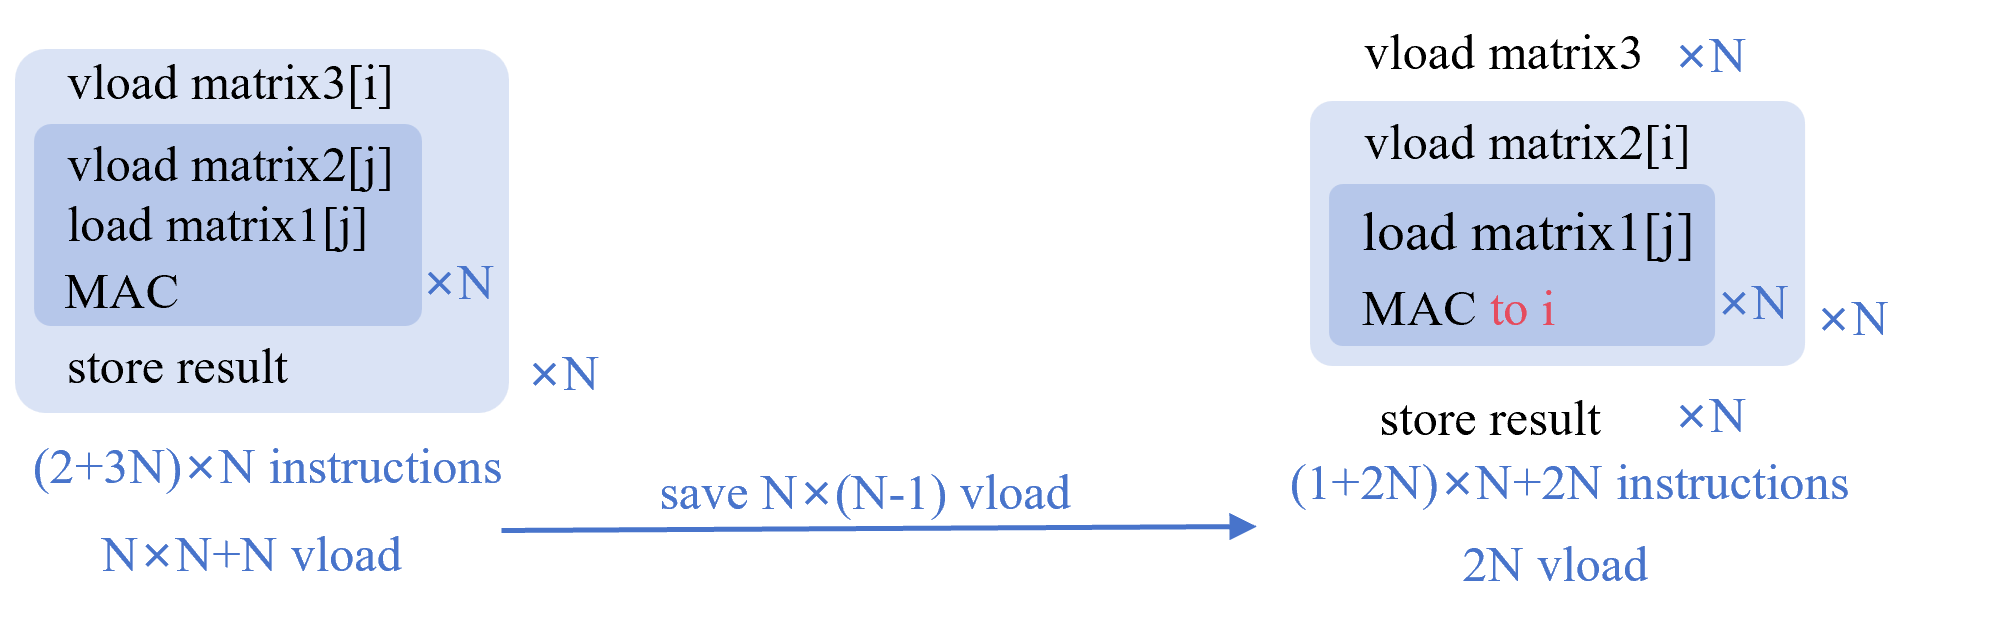
\includegraphics[width=14cm]{pic/compile_pattern.png}
    \caption{指令顺序示意图}
\end{figure}

图中N为矩阵维度,实际情况下为8,按照图中左侧的规律编写指令,需要 $3N^2+2N$ 条指令,按照右边的编写方法,需要 $2N^2+4N$条指令,
节省了 $N(N-1)$ 条矢量加载指令。考虑到矢量存储器的读取代价大于标量存储器,因此优化后的方法提升了计算速度,也有效地减小了访存延时和功耗。
优化的代价是需要将矩阵3完全存入寄存器中,占用了较多寄存器空间。

\section{总结}
本次实验实现了一个支持矢量扩展指令集的矢量处理器。设计了扩展指令集和新的硬件,并且用自己设计的指令集实现了8*8矩阵的乘加运算。
优化方面,对汇编代码进行了优化,减少了访存的次数,特别是延时功耗开销较大的矢量存储器访问次数,减少了指令数量,提高了运算效率。

通过本次实验,我进一步了解了RISCV的流水线架构中各指令的执行方式,以及指令间数据依赖的解决办法,通过前馈减少了流水线气泡的产生。


\end{document}